\documentclass[12pt]{article}
\usepackage{amsmath,amsfonts,nicefrac}
\usepackage{graphicx}
\usepackage{enumerate}
\usepackage{natbib}
\usepackage{url} % not crucial - just used below for the URL 
\usepackage{ifthen}
\usepackage{subcaption}

%\pdfminorversion=4
% NOTE: To produce blinded version, replace "0" with "1" below.
\newcommand{\blind}{1}
% DON'T change margins - should be 1 inch all around.
%\addtolength{\oddsidemargin}{-.5in}%
%\addtolength{\evensidemargin}{-.5in}%
%\addtolength{\textwidth}{1in}%
%\addtolength{\textheight}{-.3in}%
%\addtolength{\topmargin}{-.8in}%

\usepackage[margin=0.5in]{geometry}
\usepackage[table]{xcolor}% http://ctan.org/pkg/xcolor

\newcommand{\cl}[2]{\cellcolor{#1!#2}}
\newcommand{\inc}[2]{ \ifthenelse{\equal{#1}{1}}{\input{./sections/#2}}{ } }



\begin{document}

\def\spacingset#1{\renewcommand{\baselinestretch}%
{#1}\small\normalsize} \spacingset{1}


%%%%%%%%%%%%%%%%%%%%%%%%%%%%%%%%%%%%%%%%%%%%%%%%%%%%%%%%%%%%%%%%%%%%%%%%%%%%%%

\if1\blind
{
  \title{\bf A Strategy for Structured Use of Bayesian Sequential Monitoring in Clinical Trials}
  \author{Evan Kwiatkowski\textsuperscript{$\dagger$}, 
	        Eugenio Andraca-Carrera\textsuperscript{$\ddagger$},\\
					Mat Soukup\textsuperscript{$\ddagger$},
					\medskip Matthew A. Psioda\textsuperscript{$\dagger$}\thanks{The authors gratefully acknowledge \textit{please remember to list all relevant funding sources in the unblinded version}}\\
	  %
	  $\dagger$ Department of Biostatistics,
		University of North Carolina, \\
		McGavran-Greenberg Hall, CB\#7420, \\
		%
		\medskip Chapel Hill, North Carolina, U.S.A.\\
    $\ddagger$ Division of Biometrics VII, Office of Biostatistics \\
		           Center for Drug Evaluation and Research, \\
							 US Food and Drug Administration, \\
							 Silver Spring, Maryland, USA \\									
		}
  \maketitle
} \fi

\if0\blind
{
  \bigskip
  \bigskip
  \bigskip
  \begin{center}
    {\LARGE\bf Title}
\end{center}
  \medskip
} \fi

\bigskip
\begin{abstract}
Conclusions from Bayesian sequential monitoring are coherent when specification of prior distributions are intuitively related to the research objectives. A compelling level of evidence is required to terminate enrollment for either efficacy or futility. This paper defines monitoring priors using generalized normal distributions parameterized via three specified quantities (mode and two tail probabilities), which reflect prior belief defined using a consistent definition of compelling level of evidence. These concepts are demonstrated through simulations based on a single-arm proof-of-activity trial in pediatric ulcerative colitis and a parallel two-group design in pediatric lupis.
\end{abstract}

\noindent%
{\it Keywords:}  Generalized normal distribution, monitoring priors, real world evidence
\vfill

\newpage
\spacingset{1.5} % DON'T change the spacing!

\section{Introduction}

A goal of the 21st Century Cures Act \citep{USCongress2016} is to expedite the approval process for new drugs and devices through the incorporation of real-world evidence into clinical trial data summaries. Similarly, an objective of the Prescription Drug User Fee Act VI  is to enhance the capacity to review ``complex adaptive, Bayesian, and other novel clinical trial designs." \citep{FDA2017} Bayesian designs are natural for incorportating external evidence through prior distributions. This is useful in areas where clinical trials would take a lot of time due to slow enrollment or long follow-up periods, and where relevant external data exists. For example, a treatment for a rare pediatric disease might have difficulties with enrollment, and there may be relevant data from adult trials which could augument the trial findings and lead to a conclusion of efficacy sooner. Group sequential designs also have the possible benefits of leading to conclusions earlier, saving time and resources, as well as reducing the exposure of patients to inferior treatments. Bayesian sequential designs which incorporate external evidence therefore have a much increased capacity to expedite the approval process for effective treatments, but they most be carefully planned. The effects of interim analyses and the informativeness of the priors must be well understood. This paper presents a structured or default way to determine prior distributions based on the trial design. Our major contribution is to present methods for the default or automatic selection of prior distributions in a way that is applicable to a wide array of clinical trial designs.


The likelihood principle asserts that any data with the same likelihood function should lead to the same conclusion \citep{Berger1988}. In the context of sequential analysis of clinical trials, the stopping rule that led to the termination of data collection is irrelevant to the conclusion \citep{Barnard1947,Anscombe1963,Cornfield1966a,Cornfield1966b}. It is most succinctly as ``It is entirely appropriate to collect data until a point has been proven or disproven, or until the data collector runs out of time, money, or patience."\citep{Edwards1963}. Bayesian conclusions are not affected by frequent or even continual monitoring of the data, and such interim analyses should be encouraged to terminate data collection if appropriate \citep{Berry1989,Berry1993,Spiegelhalter1994}.

Interpretation of conclusions from the Bayesian perspective is natural when specification of prior distributions are intuitively related to the research objectives (e.g. skeptical and enthusiastic priors)  \citep{Freedman1989,Freedman1992,Spiegelhalter1993,Fayers1997} which is necessary for regulatory agencies \citep{Parmar1993}. Bayesian monitoring is further formalized by specifying the loss function via decision theory \citep{Carlin1998}.

The most common Bayesian metrics for assessing evidence at interim analyses are posterior probabilities and predictive probabilities, and the choice of metric depends on research objective. Posterior probabilities assess the level of evidence in favor of the null or alternative hypothesis, and predictive probabilities determine the capacity for the trial to show convincing evidence in favor of the alternative hypothesis if more outcomes are ascertained. This paper uses posterior probabilities to highlight how the level of evidence at interim analyses is linked to monitoring prior specification.

Frequentist group sequential designs use spending functions associated with Type I and Type II error \citep{Pocock1977,OBrien1979}. While it is possible to calibrate a Bayesian design to have exact pre-specified frequentist properties \citep{Kopp-Schneider2019}, this re-introduces inflexibility (e.g. interim analyses must be pre-specified) that is unnecessary using a fully Bayesian method. Therefore, the objective is to present operating characteristics generally that are ``well-calibrated" \citep{Grieve2016} but not motivated by strict adherence to pre-specified thresholds.

This paper is organized as follows: Section \ref{sec:methods} contains a brief review of Bayesian hypothesis testing using posterior probabilities, and describes the method for defining monitoring and inference priors. Examples are in Section \ref{sec:examples}, with Section \ref{sec:example1} containing a one-arm study and Section \ref{sec:example2} a two-arm study.

\section{Methods}\label{sec:methods}
%\subsection{Monitoring versus Estimation Priors}
%\begin{itemize}
% \item Define generally in terms of $\boldsymbol\theta = \left( \gamma, \boldsymbol\psi  \right)$ where $\gamma$ is a parameter of interest
%       and $\boldsymbol\psi$ is a nuisance parameter (possible vector valued).
% \item Define \textit{Monitoring} Priors and \textit{Inference} Priors.
% \item Make connection between Inference priors and two-part mixture prior and BMA.
% \item Define \textit{Skeptical} and \textit{Enthusiastic} monitoring priors and how each would be used.
% \item I would have a generic graphic to illustrate the types of priors and the mixture.
% %\item Motivate in the context of a simple example (i.e., single parameter binary example).
%\end{itemize}

\subsection{Preliminaries}\label{sec:preliminaries}
\subsubsection{Bayesian hypothesis testing using posterior probabilities}
Consider a one-arm trial with a single measured outcome per patient. The objective is to make inference on a single unknown quantity. Let $\mathbf{D}$ be a random variable representing the data collected in the trial with density $p(\mathbf{D}|\theta)$, where $\theta$ is the parameter of interest with sample space $\theta\in\Theta$. 
%
For example, in the context of a simple binary outcome (e.g., objective response to treatment) based on sample size $n$, $\mathbf{D} = \left(y_1,...,y_n\right)$ may correspond to the $n$ indicators for whether or not subjects responded to a treatment and $\theta\in[0,1]$ may correspond to an assumed common probability of response.

Formal Bayesian hypothesis testing requires the specification of prior probabilities on the hypotheses (e.g., $p(H_i)$ for $i=0,1$)
and prior distributions for $\theta$ for each hypothesis (e.g. $\pi\left(\theta \big| H_i\right)$ for $i=0,1$). 
%
Consider the hypotheses $H_0:\theta\in\Theta_{0}$ versus $H_1:\theta\in\Theta_{1}$ where $\Theta_{0}\bigcup \Theta_{1} = \Theta$ and $\Theta_{0} \bigcap \Theta_{1} = \emptyset$. 

The posterior probability of hypothesis $H_i$ is 
\begin{align}
p(H_i|\mathbf{D})&=\frac{p(\mathbf{D}|H_i)\cdot p(H_i)}{p(\mathbf{D}|H_0)\cdot p(H_0)+p(\mathbf{D}|H_1)\cdot p(H_1)}\\
&=\frac{\int_{\Theta_i} p(\mathbf{D}|\theta,H_i)\pi(\theta|H_i)d\theta\cdot p(H_i)}{p(\mathbf{D}|H_0)\cdot p(H_0)+p(\mathbf{D}|H_1)\cdot p(H_1)}.
\end{align}

The posterior probability of the \textit{event defining $H_i$} is
\begin{align}\label{eq:equation1}
P(\theta\in\Theta_i|\mathbf{D})
&=\int_{\Theta_i}p(\theta|\mathbf{D})d\theta\\
&=\frac{\int_{\Theta_i}p(\mathbf{D}|\theta)\pi (\theta)d\theta}{\int_{\Theta}p(\mathbf{D}|\theta)\pi(\theta) d\theta}\\
&=\frac{\int_{\Theta_i}p(\mathbf{D}|\theta)\pi (\theta|\theta\in\Theta_i)d\theta\cdot P(\theta\in\Theta_i)}{\int_{\Theta}p(\mathbf{D}|\theta)\pi(\theta) d\theta},
\end{align}
where $P(\theta\in\Theta_i)=\int_{\Theta_i}\pi(\theta)d\theta$. 

When $p(H_i) =P(\theta\in\Theta_i)$ and 
$\pi\left(\theta \big| H_i\right) = \pi\left(\theta\big|\theta \in \Theta_i\right)$ for $i=0,1$,
it follows that the posterior probability of the event defining the alternative hypothesis and the posterior
probability of the alternative hypothesis are equivalent. 

Consistent with the specifications of $p(H_i)$ and $\pi\left(\theta \big| H_i\right)$ as described above, in what follows we will refer to 
the quantity $P(\theta\in\Theta_1|\mathbf{D})$ as the posterior probability of $H_i$ for ease of exposition.

\subsubsection{Compelling level of evidence}
Define $\epsilon$ as the \textit{residual uncertainty} of $H_i$ being true relative to the competing hypothesis, and define $1-\epsilon\in(0,1)$ as the threshold for \textit{a compelling level of evidence} that some claim about $\theta$ is true. We say that an individual is \textit{all but convinced} that $H_i$ is true given the observed data if they believe that
\begin{align}\label{eq:compellingevidence}
P(\theta\in\Theta_i|\mathbf{D})> 1-\epsilon.
\end{align} 

Furthermore, $1-\epsilon\in(0,1)$ can be used as a threshold for \textit{a compelling a priori belief} that some claim about $\theta$ is true before the beginning of the trial. We say that an individual is \textit{all but convinced} that $H_i$ is true a priori if they believe that
\begin{align}\label{eq:compellingapriori}
P(\theta\in\Theta_i)>1-\epsilon.
\end{align} 

\subsubsection{Skeptical and Enthusiastic Monitoring Priors}\label{sec:MP}
Continuing the trial setup from Section \ref{sec:preliminaries}, suppose every subject receives active treatment during the follow-up period from enrollment to study completion. The length of follow-up is the same for each subject. Subjects are enrolled progressively such that there is a time when there are both subjects with completed outcomes and subjects undergoing follow-up. In this paper we introduce two types of prior: monitoring and inference priors. 

The purpose of monitoring priors to is help answer the question ``Is the evidence compelling enough to end the trial early?'' Monitoring priors are used for interim analyses on the data from subjects who completed follow-up while additional outcomes are pending. A promising interim result that shows clear efficacy of the treatment would justify stopping the enrollment of additional subjects, while enrolled subjects would continue receiving the presumed effective treatment during the follow-up period. A discouraging interim result that shows clear futility of the treatment would justify stopping the enrollment of additional subjects, and may call for enrolled patients undergoing follow-up to stop receiving the presumed ineffective treatment. 

To have either efficacy or futility to be ``clear" the evidence must be convincing to individuals with diverse opinions of $\theta$. The judgment of efficacy must be convincing even to an individual who was initially skeptical about the benefit of the treatment. Likewise, the judgment of futility must be convincing to an individual was initially optimistic. For this reason monitoring priors generally represent relatively extreme (but still plausible) beliefs about $\theta$. If a skeptic has become confident that the treatment is efficacious, 
that implies essentially anyone with some degree of equipoise would also be convinced, hence individuals with diverse opinions have a consensus. Alternatively, if an enthusiast has become convinced that the treatment is ineffective, then essentially everyone will share that opinion. 

%It has been said that ``the purpose of a trial is to collect data that bring to conclusive consensus at termination opinions that had been diverse and indecisive at the \textit{outset}" (Kass and Greenhouse (1989), emphasis added). 
%
%Such opinions may be characterized through specification of different priors that vary in terms of the set of values of $\theta$ that are most likely and the mass allocated to specific regions of the parameter space (e.g., $\theta\in\Theta_i$).
%\textcolor{orange}{There is only one research objective and that is to determine which of the two hypotheses is likely to be true.}
%

Monitoring priors will be defined based on the concepts of compelling a prior belief defined in Section \ref{sec:preliminaries}. Continuing the trial setup from Section \ref{sec:preliminaries}, suppose that $\theta$ corresponds to a probability of desired response, and the null hypothesis is $H_0:\theta\leq\theta_0$ where $\theta_0$ is the expected null response among untreated subjects. 
%
Let $\theta_1>\theta_0$ be a highly efficacious response probability.
%

We define an enthusiastic prior $\pi_{E}(\theta)$ as a prior that is centered around $\theta_1$ and reflects the belief of an individual that is \textit{all but convinced} that $H_i$ is true a priori, that is, 
\begin{align}\label{eq:enthprior}
P(\theta >\theta_0| \pi_{E})>1-\epsilon.
\end{align} 

Consider a similarly defined skeptical prior $\pi_{S}(\theta)$ that is centered around $\theta_0$ and reflects the belief of an individual that is \textit{all but convinced} that $H_0$ is true a priori, that is, $P(\theta\leq\theta_0| \pi_{S})>1-\epsilon$. Having this belief demonstrates such an extreme disbelief in the possibility of a positive effect that conducting the trial at all would be viewed as dubious. This is analogous to specifying a prior model probability on $H_0$ that is $1-\epsilon$ and that is not consistent with their being clinical equipoise about the hypotheses; such extreme skepticism is not rational if a trial is to be conducted. 

Instead, we define the skeptical prior $\pi_S(\theta)$ to be centered around $\theta_0$ and reflects the belief of an individual that is \textit{all but convinced} that a highly efficacious response probability is unlikely, that is,  
\begin{align}\label{eq:skptprior}
P(\theta>\theta_1| \pi_{S})<\epsilon.
\end{align}

The enthusiastic and skeptical conditions defined in (\ref{eq:enthprior}), (\ref{eq:skptprior}) will be referred to as tail-probability constraints.

\subsubsection{Criteria for Early Stoppage}
The use of monitoring based on changing the opinion of skeptical and enthusiastic priors has been described as overcoming a handicap (\cite{Freedman1989}) and providing a brake (\cite{Fayers1997}) on the premature termination of trials, or constructing ``an adversary who will need to be disillusioned by the data to stop further experimentation" (\cite{Spiegelhalter1994}). Early termination of enrollment is appropriate if diverse prior opinions about $\theta$ would be in agreement given the interim data (e.g. the skeptical and enthusiastic person reach the same conclusion). 

The skeptic, whose prior belief is reflected in (\ref{eq:skptprior}), becomes convinced the treatment is effective if there is compelling evidence that $\theta>\theta_0$ is true (\ref{eq:compellingevidence}), that is, 
\begin{align}
P(\theta<\theta_1|\pi_{S})>1-\epsilon \Rightarrow P(\theta>\theta_0| \mathbf{D},\pi_{S})>1-\epsilon.
\end{align}

Consider $\theta<\frac{\theta_0+\theta_1}{2}$ to be a response that is less than the highly efficacious response probability $\theta_1$. The enthusiast, whose prior belief is reflected in (\ref{eq:enthprior}), becomes convinced the treatment is ineffective, or not as effective as anticipated, if there is compelling evidence that $\theta<\frac{\theta_0+\theta_1}{2}$, that is, 
\begin{align}
P(\theta>\theta_0|\pi_{E})>1-\epsilon\Rightarrow P\left(\theta<\frac{\theta_0+\theta_1}{2}\Big| \mathbf{D},\pi_{E}\right)>1-\epsilon.
\end{align}
%
\subsection{Monitoring Prior Specification}
\subsubsection{Normal Family of Distributions}
The enthusiastic and skeptical priors defined in (\ref{eq:enthprior}), (\ref{eq:skptprior}) each have a required center (modal value) and tail-probability constraint, however, there are still many ways to parameterize such distributions. The specification of the mean and variance of a normal distribution completely specifies the modal value and tail-probability constraints, and is therefore sufficient for defining enthusiastic and skeptical priors.

Consider the normal distribution for a random variable $\theta$
\begin{align}
p(\theta;\mu,\sigma)=\frac{1}{\sigma\sqrt{2\pi}}exp\left\{-\frac{1}{2}\left(\frac{x-\mu}{\sigma}\right)\right\}^2
\end{align}
with quantile function for $p\in(0,1)$
\begin{align}
Q(p;\mu,\sigma)=\mu+\sigma\sqrt{2}erf^{-1}(2p-1)
\end{align}
where $erf^{-1}$ is the inverse of the error function.

Consider creating an enthusiastic prior that is centered around $\theta_1$ and satisfies the tail-probability condition of (\ref{eq:enthprior}), which is expressed as $Q(\theta_0;\mu=\theta_1,\sigma)=\epsilon$. This is the normal distribution 
\begin{align}\label{eq:enthsd}
\pi_E(\theta)\sim N\left(\mu=\theta_1,\sigma=\frac{\theta_0-\theta_1}{\sqrt{2}erf^{-1}(2\epsilon-1)}\right)
\end{align}

By symmetry, a skeptical prior that is centered around $\theta_0$ and satisfies the tail-probability condition of (\ref{eq:skptprior}), which is expressed as $Q(\theta_1;\mu=\theta_0,\sigma)=1-\epsilon$, is the normal distribution with $\mu=\theta_0$ and the same variance as (\ref{eq:enthsd}).

\subsubsection{The Generalized Normal Family of Distributions}
For additional flexibility, we will consider the generalized normal distribution for prior specification. Consider the generalized normal distribution for a random variable $\theta$ 
\begin{align}\label{eq:generalizednormalkernel}
p(\theta;\mu,\alpha,\beta)=\frac{\beta}{2\alpha\Gamma(1/\beta)}\exp\left\{-\left(\frac{|\theta-\mu|}{\alpha}\right)^\beta\right\}
\end{align} where $\mu\in\mathbb{R}$ is a location parameter, $\alpha>0$ is a scale parameter, and $\beta>0$ is a shape parameter. Note that $\beta=2$ corresponds to the normal distribution. 

The quantile function for $p\in (0,1)$ is 
\begin{align}
Q(p;\mu,\alpha,\beta)=sign(p-0.5) g\left(2|p-0.5|;\frac{1}{\beta}\left(\frac{1}{\alpha}\right)^{\beta}\right)^{1-\beta}+\mu,
\end{align}
where $g\left(2|p-0.5|;\frac{1}{\beta}\left(\frac{1}{\alpha}\right)^{\beta}\right)$ refers to the inverse CDF for a gamma distribution with shape $\frac{1}{\beta}$ and rate $(\frac{1}{\alpha})^\beta$ evaluated at $2|p-0.5|$.

Consider creating an enthusiastic prior that is centered around $\theta_1$ and satisfies the tail-probability condition of (\ref{eq:enthprior}), which is expressed as 
\begin{align}\label{eq:enthprior_tail1}
Q(\theta_0:\mu=\theta_1,\alpha,\beta)=\epsilon
\end{align} and that also satisfies a second tail-probability condition 
\begin{align}
Q\left(\frac{\theta_0+\theta_1}{2};\mu=\theta_1,\alpha,\beta\right)=\epsilon+\gamma \label{eq:enthprior_tail2}
\end{align}
for $\gamma>\epsilon$. There is a unique combination of $\alpha$ and $\beta$ that satisfy (\ref{eq:enthprior_tail1}) and (\ref{eq:enthprior_tail2}).


The modification of $\beta$ can be used to concentrate or flatten the distribution around the modal value. If $\beta<2$ then the distribution becomes more peaked relative to a normal distribution, and if $\beta>2$ then the distribution becomes flatter. Examples of skeptical and enthusiastic priors for a single parameter $\theta$ based on the trial from Section \ref{sec:preliminaries} are displayed in Figure \ref{fig:figure1}. The location and shape parameters are pre-specified, and the scale parameter is chosen to satisfy the tail-probability constraints (\ref{eq:enthprior}), (\ref{eq:skptprior}).

%Continuing the trial setup from Section \ref{sec:preliminaries}, it is necessary to truncate the generalized normal distribution to the range $[0,1]$. When truncated to the unit interval, this density becomes
%\begin{align}\label{eq:generalized_normal_univariate}
%\pi(\theta)\propto \exp\left\{-\frac{|\theta-\mu|}{\alpha}^\beta\right\} I(\theta\in[0,1]).
%\end{align} 
%

\begin{figure}\begin{center}
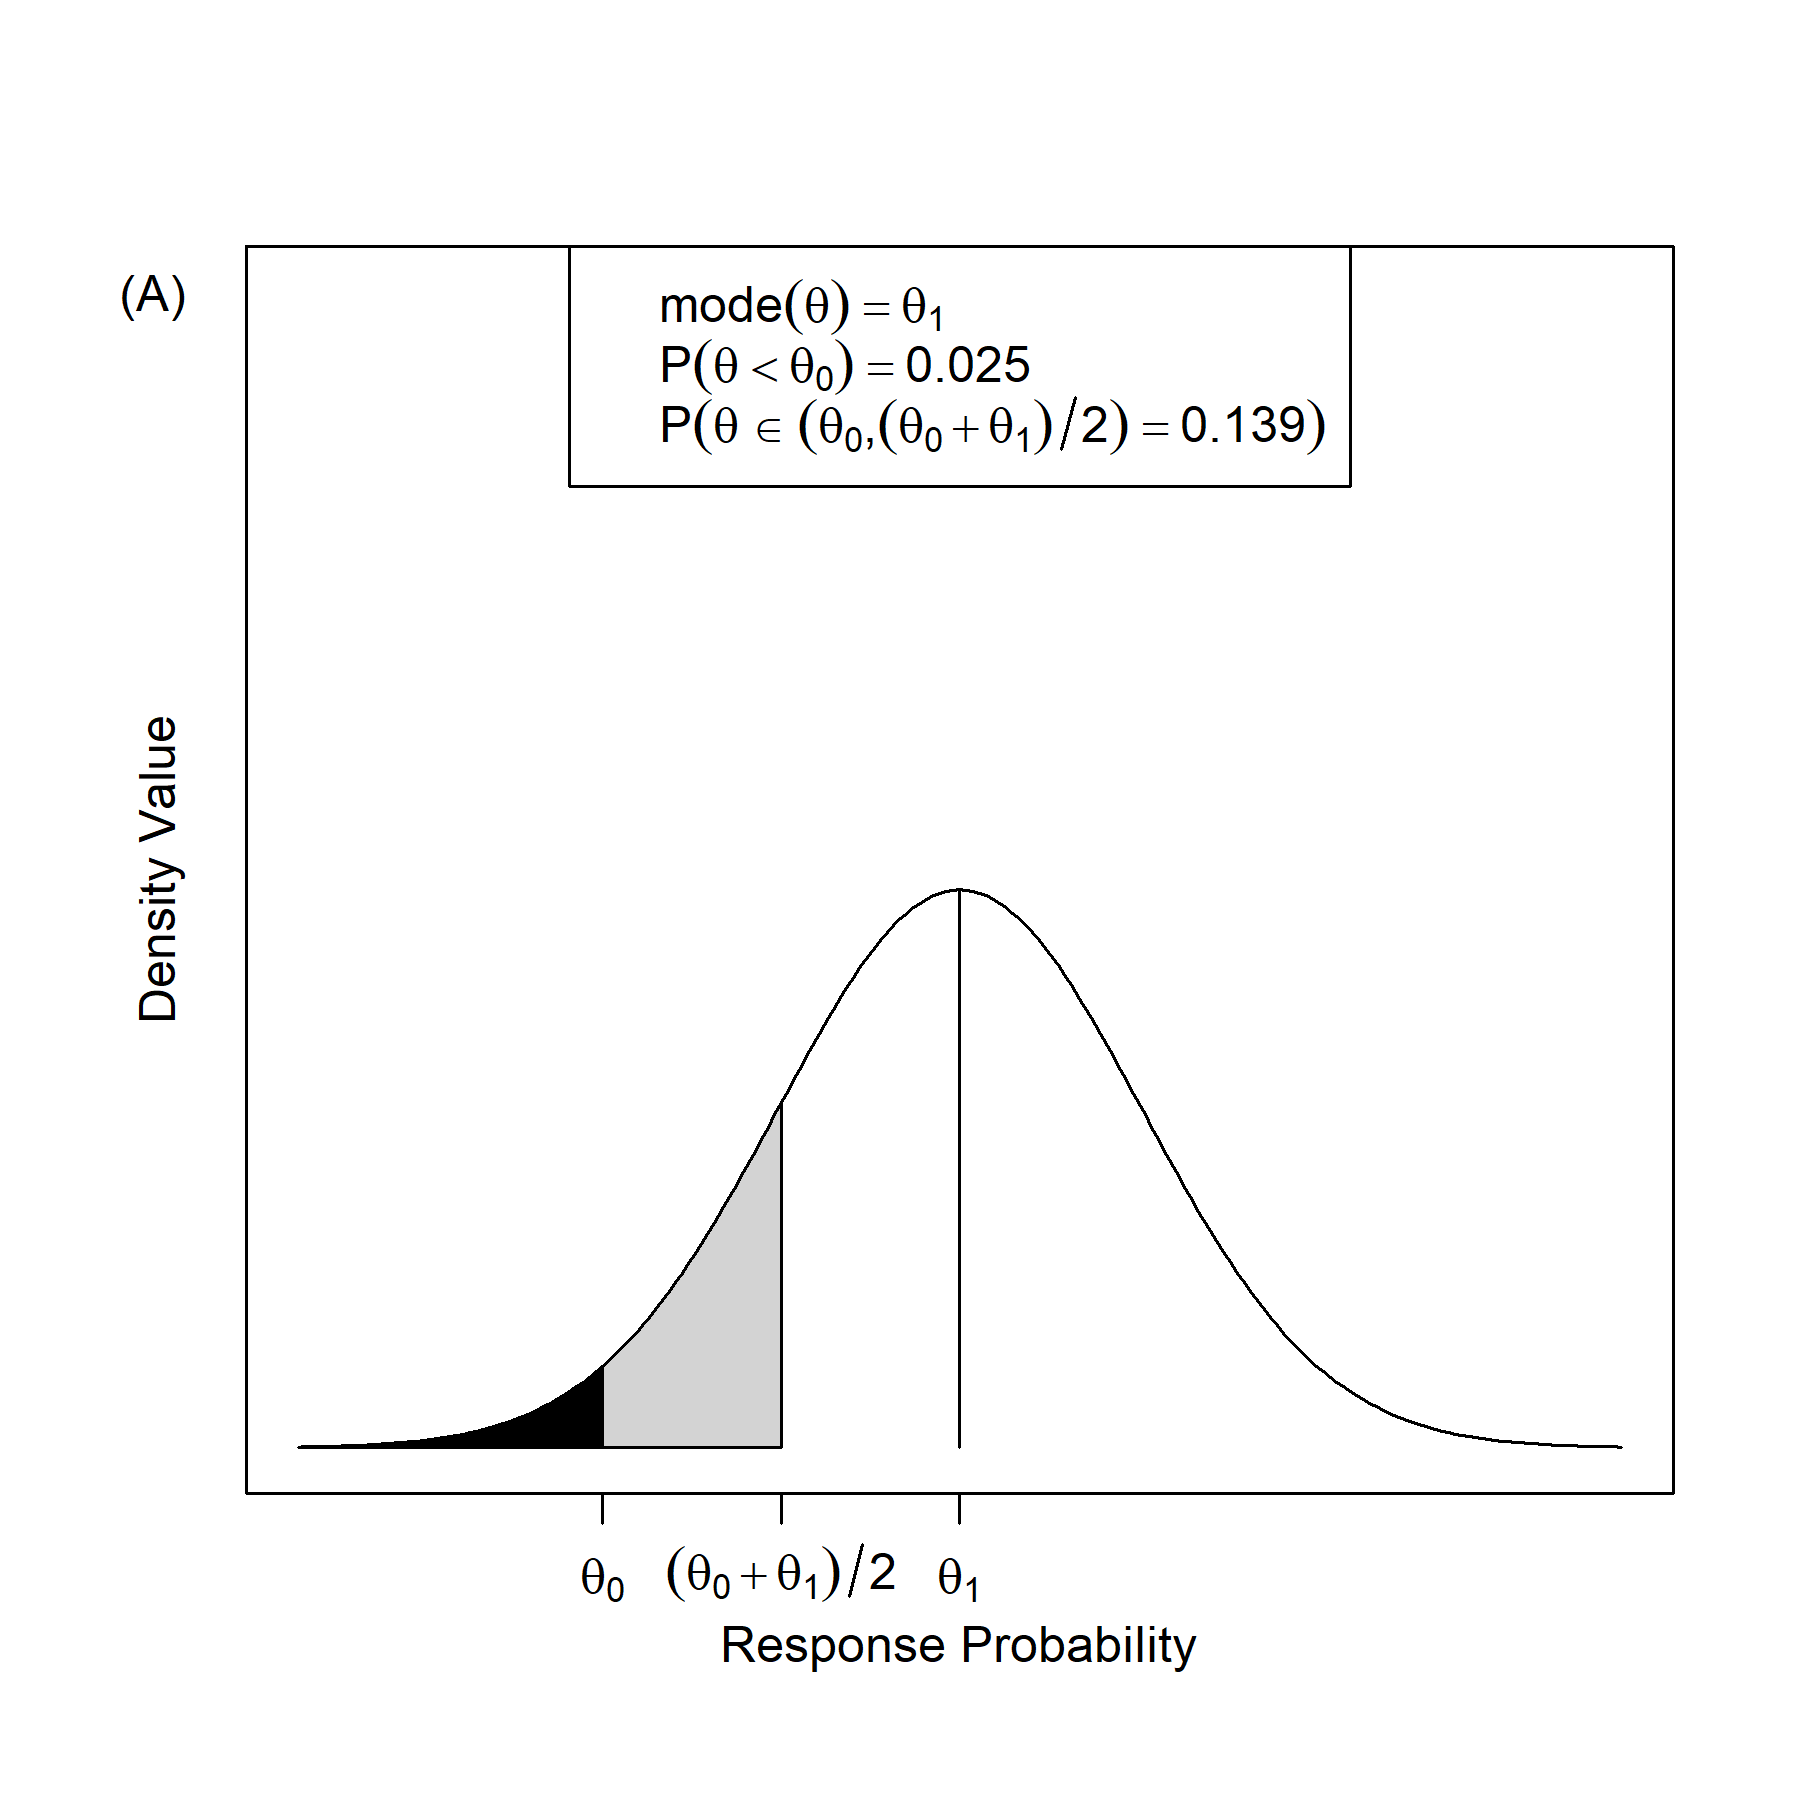
\includegraphics[width=3in]{P:/Bayesian-Sequential-Monitoring/00-paper/FIGURES/figure1a.png}
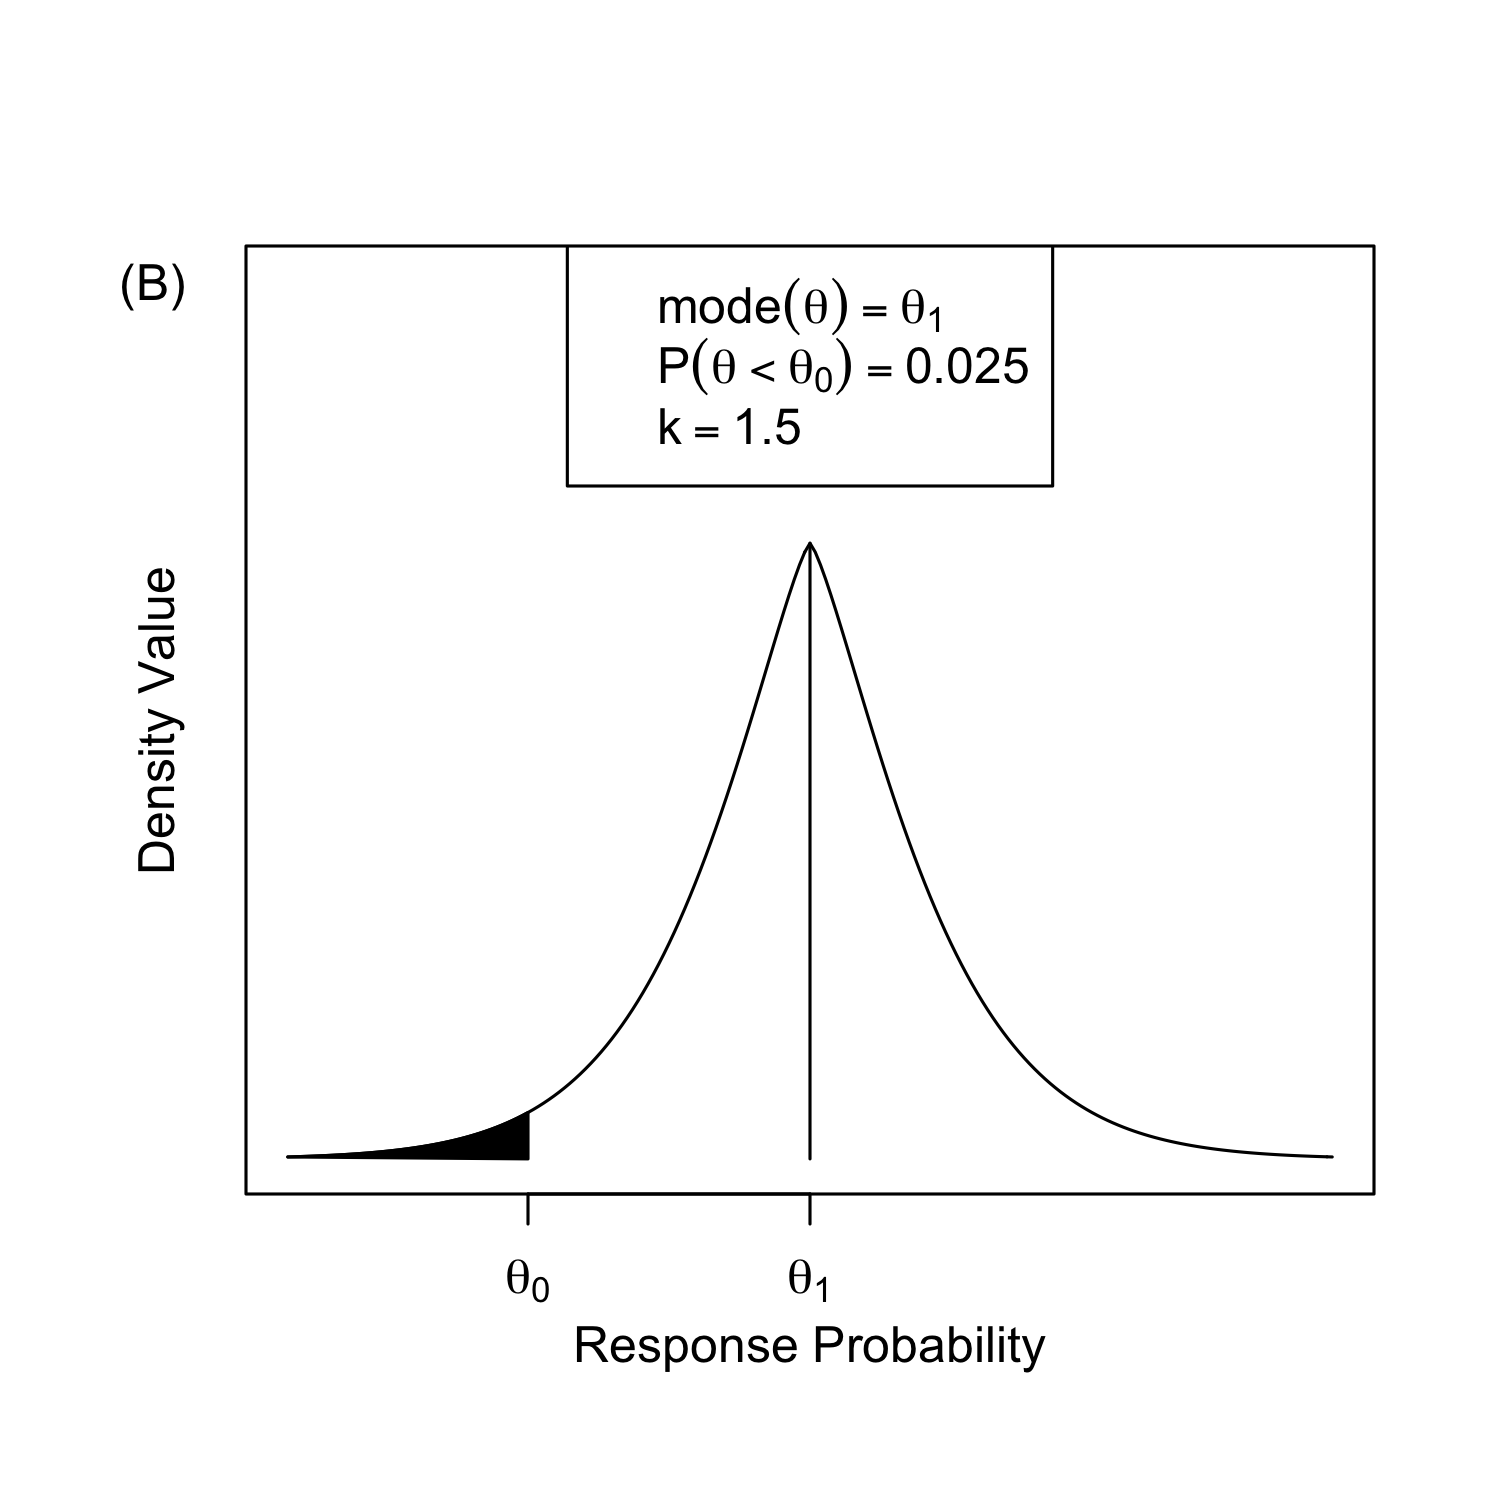
\includegraphics[width=3in]{P:/Bayesian-Sequential-Monitoring/00-paper/FIGURES/figure1b.png}

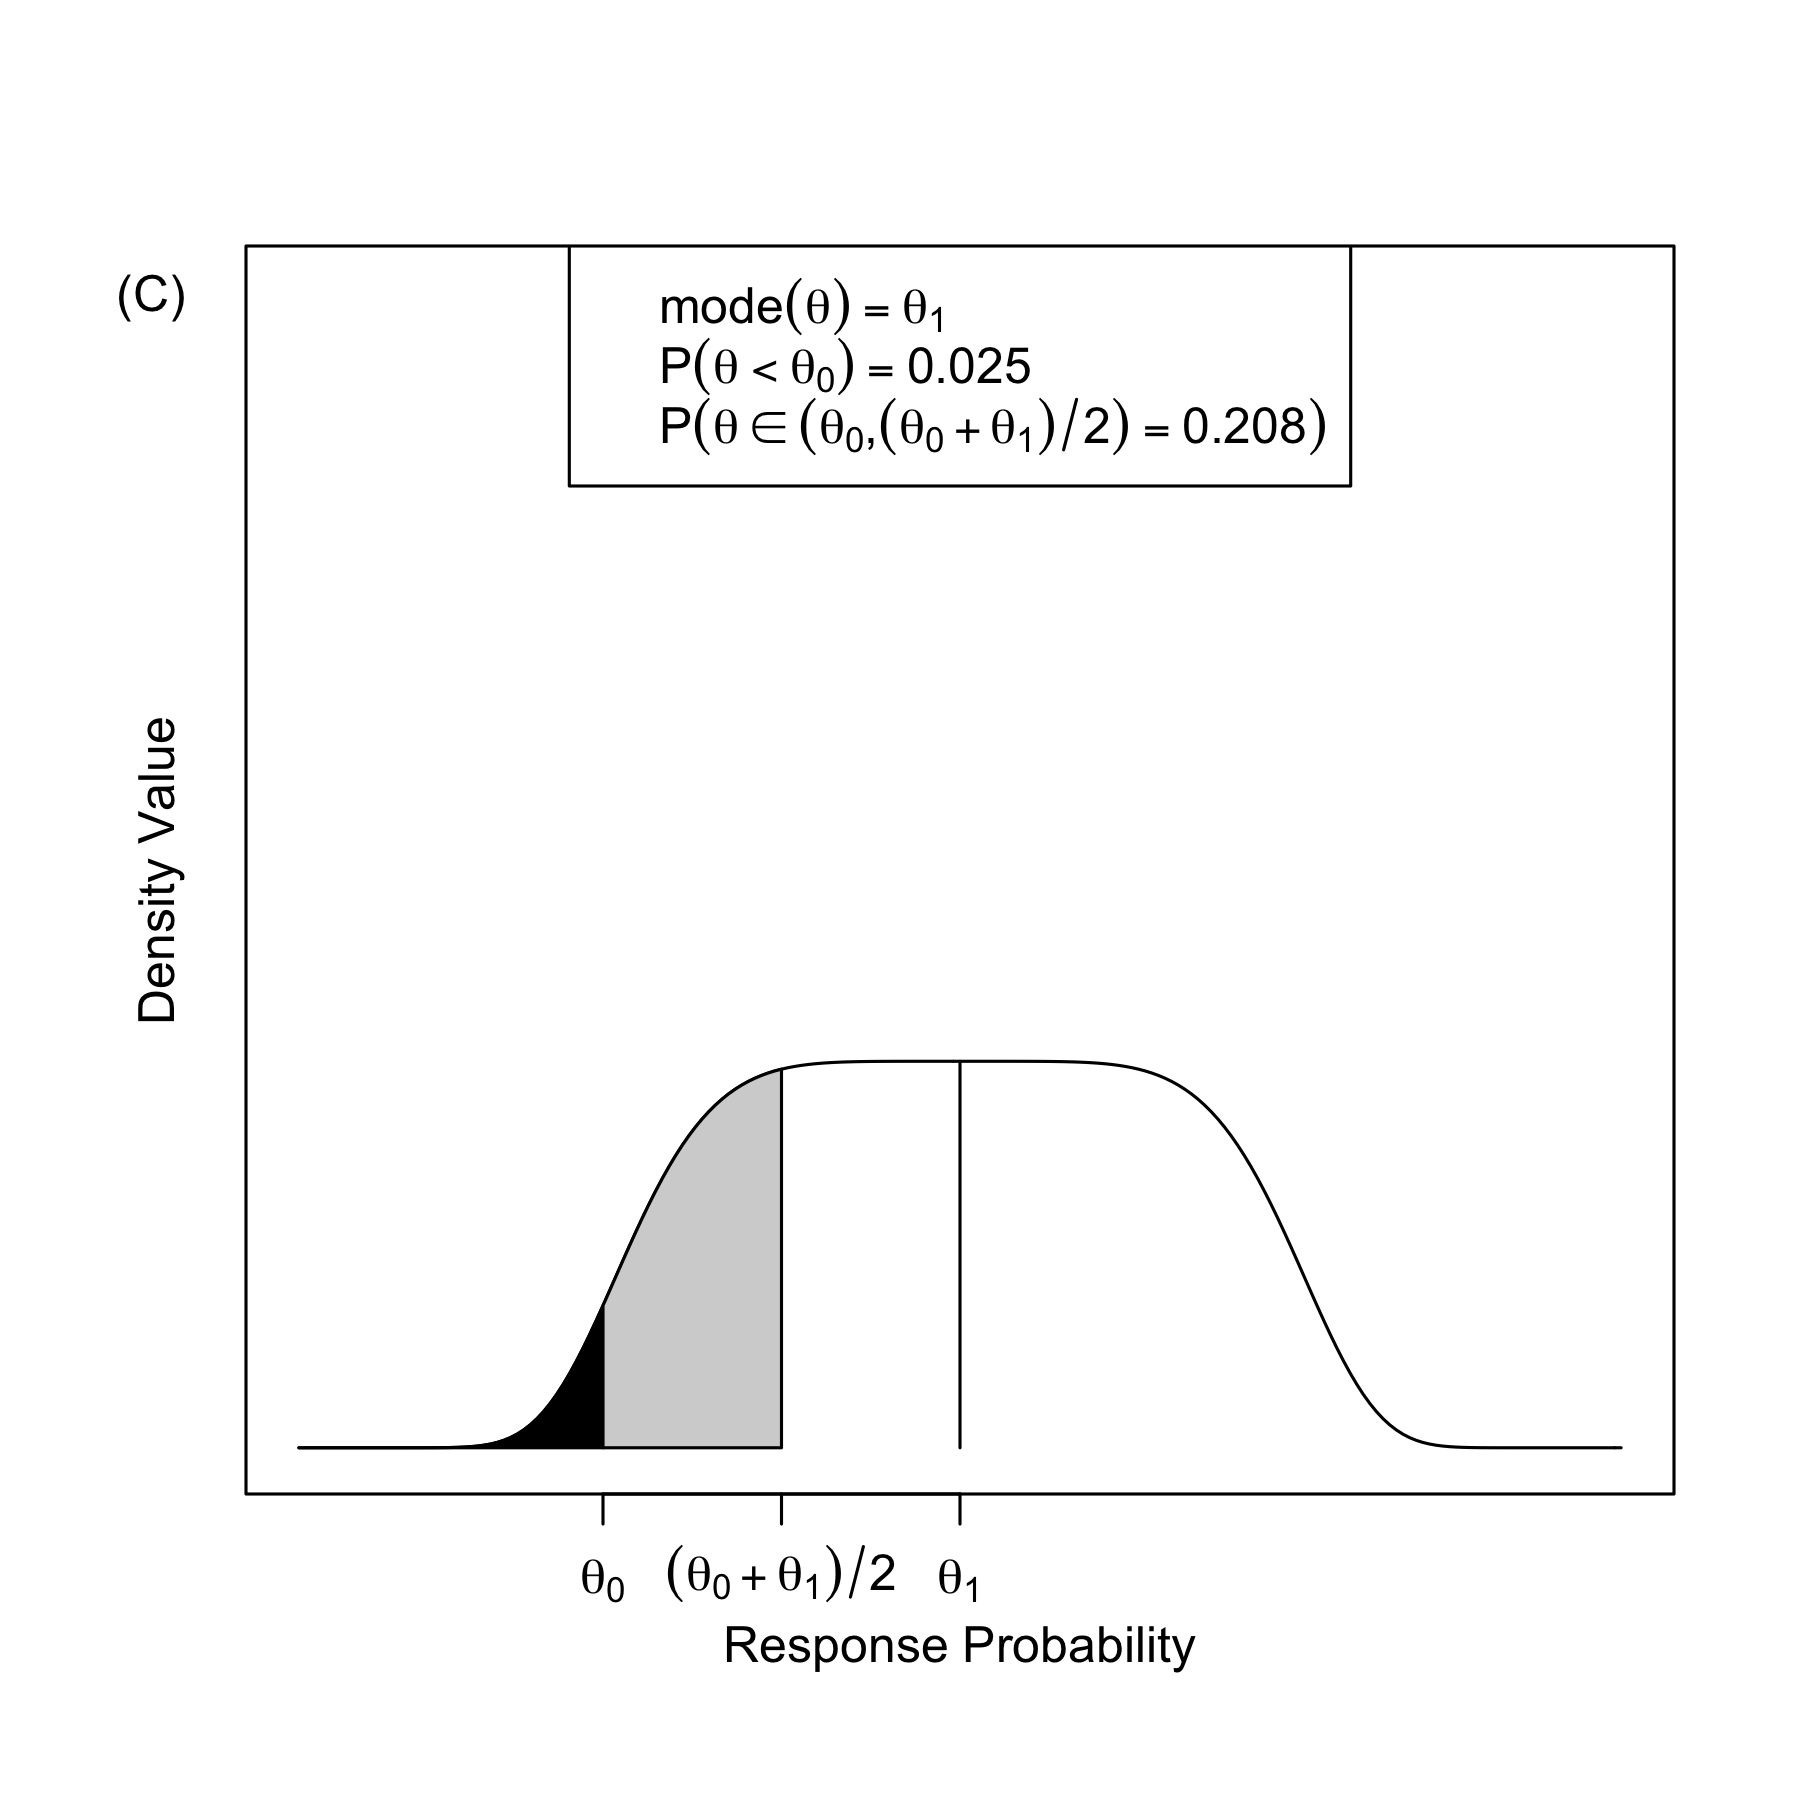
\includegraphics[width=3in]{P:/Bayesian-Sequential-Monitoring/00-paper/FIGURES/figure1c.png}
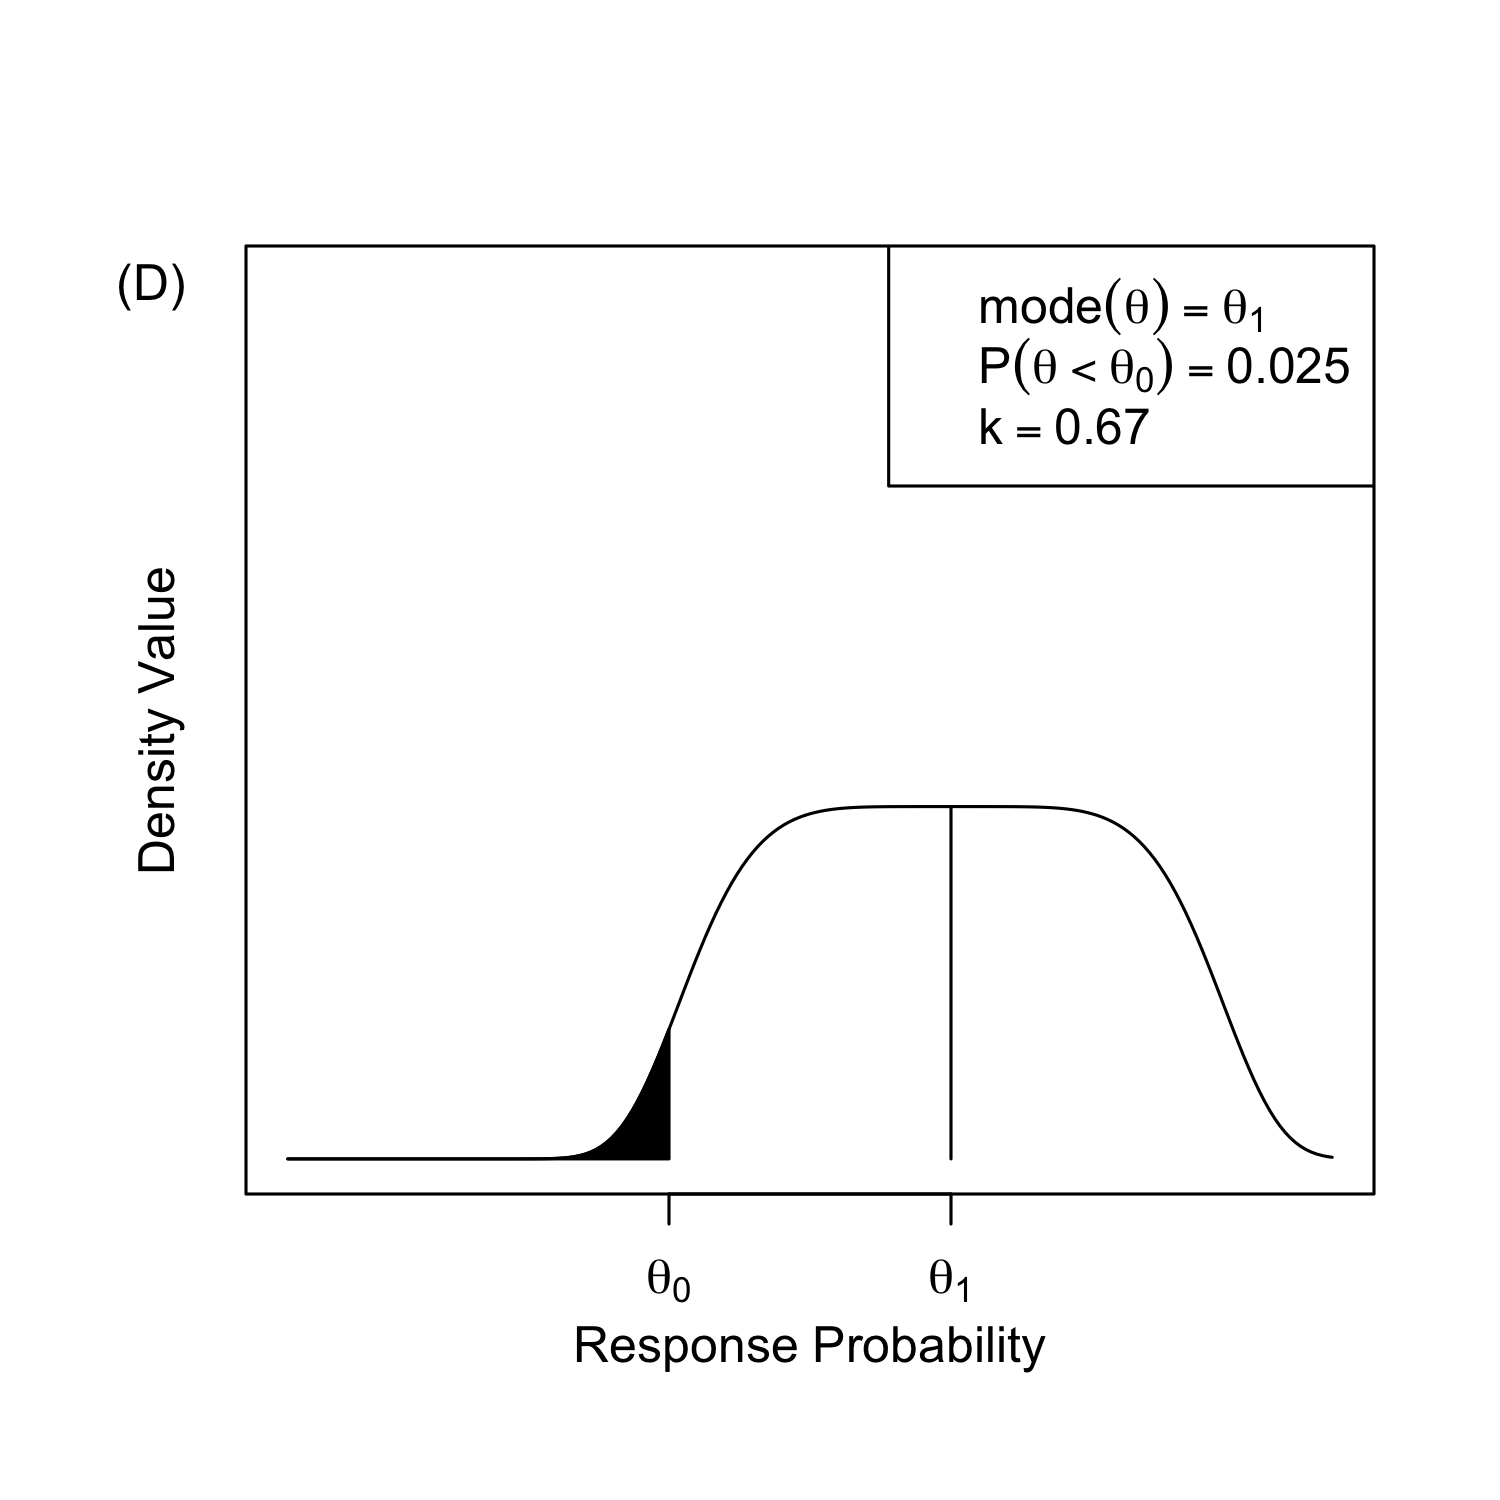
\includegraphics[width=3in]{P:/Bayesian-Sequential-Monitoring/00-paper/FIGURES/figure1d.png}

\caption{A, Skeptical prior, normal distribution. B, Skeptical prior, generalized normal distribution with added concentration around modal value. C, Enthusiastic prior, normal distribution. D, Enthusiastic prior, generalized normal distribution with added flattening around modal value.}
\label{fig:figure1}
\end{center}\end{figure}

The normal and generalized normal family of distributions can be truncated to a restricted domain that reflects the research quantity of interest (e.g. a response probability on [0,1]).
\subsubsection{Application to higher dimensions}
The generalized normal distribution can be used to parameterize skeptical and enthusiastic priors for trials with multiple unknown quantities of interest. Suppose the trial from Section \ref{sec:preliminaries} has added a control arm, and let $\theta_0$ and $\theta_1$ be the response proportions for a control and treatment group respectively. Suppose that the risk difference $\theta_1-\theta_0$ is of interest. Let $\delta_0$ denote a null risk difference and $\delta_1$ denote a highly efficacious risk difference.

Consider the following representation of the joint prior for $\theta_1$ and $\theta_0$:
\begin{align}
\pi(\theta_0,\theta_1)=&\pi(\theta_0)\times\pi(\theta_1|\theta_0). \label{eq:generalized_normal_joint}
\end{align}

Each of these components can be represented in the form of (\ref{eq:generalizednormalkernel}) by
\begin{align}
\pi(\theta_0)\propto&\exp\left\{-\left(\frac{|\theta_0-\mu_0|}{\alpha_0}\right)^{\beta_0}\right\} \label{eq:genNormPlacebo}\\
\pi(\theta_1|\theta_0)\propto&\exp\left\{-\left(\frac{|(\theta_1-\theta_0)-\delta|}{\alpha_1}\right)^{\beta_1}\right\}f(\theta_0). \label{eq:genNormRd}
\end{align}

The component $\pi(\theta_0)$ reflects prior opinion about the response rate in the placebo group, and the component $\pi(\theta_1|\theta_0)$ can be used to express pessimism or optimism in the difference in proportions $\theta_1 - \theta_0$. 

The enthusiastic prior condition from (\ref{eq:enthprior}) become
\begin{align}\label{eq:ex2enthcondition}
P(\theta_1-\theta_0>\delta_0)=1-\epsilon.
\end{align}

The skeptical prior condition from (\ref{eq:skptprior}) become
\begin{align}\label{eq:ex2skptcondition}
P(\theta_1-\theta_0<\delta_1)=1-\epsilon.
\end{align}


Examples of skeptical and enthusiastic priors are displayed in Figure \ref{fig:figure5}.

\begin{figure}\begin{center}
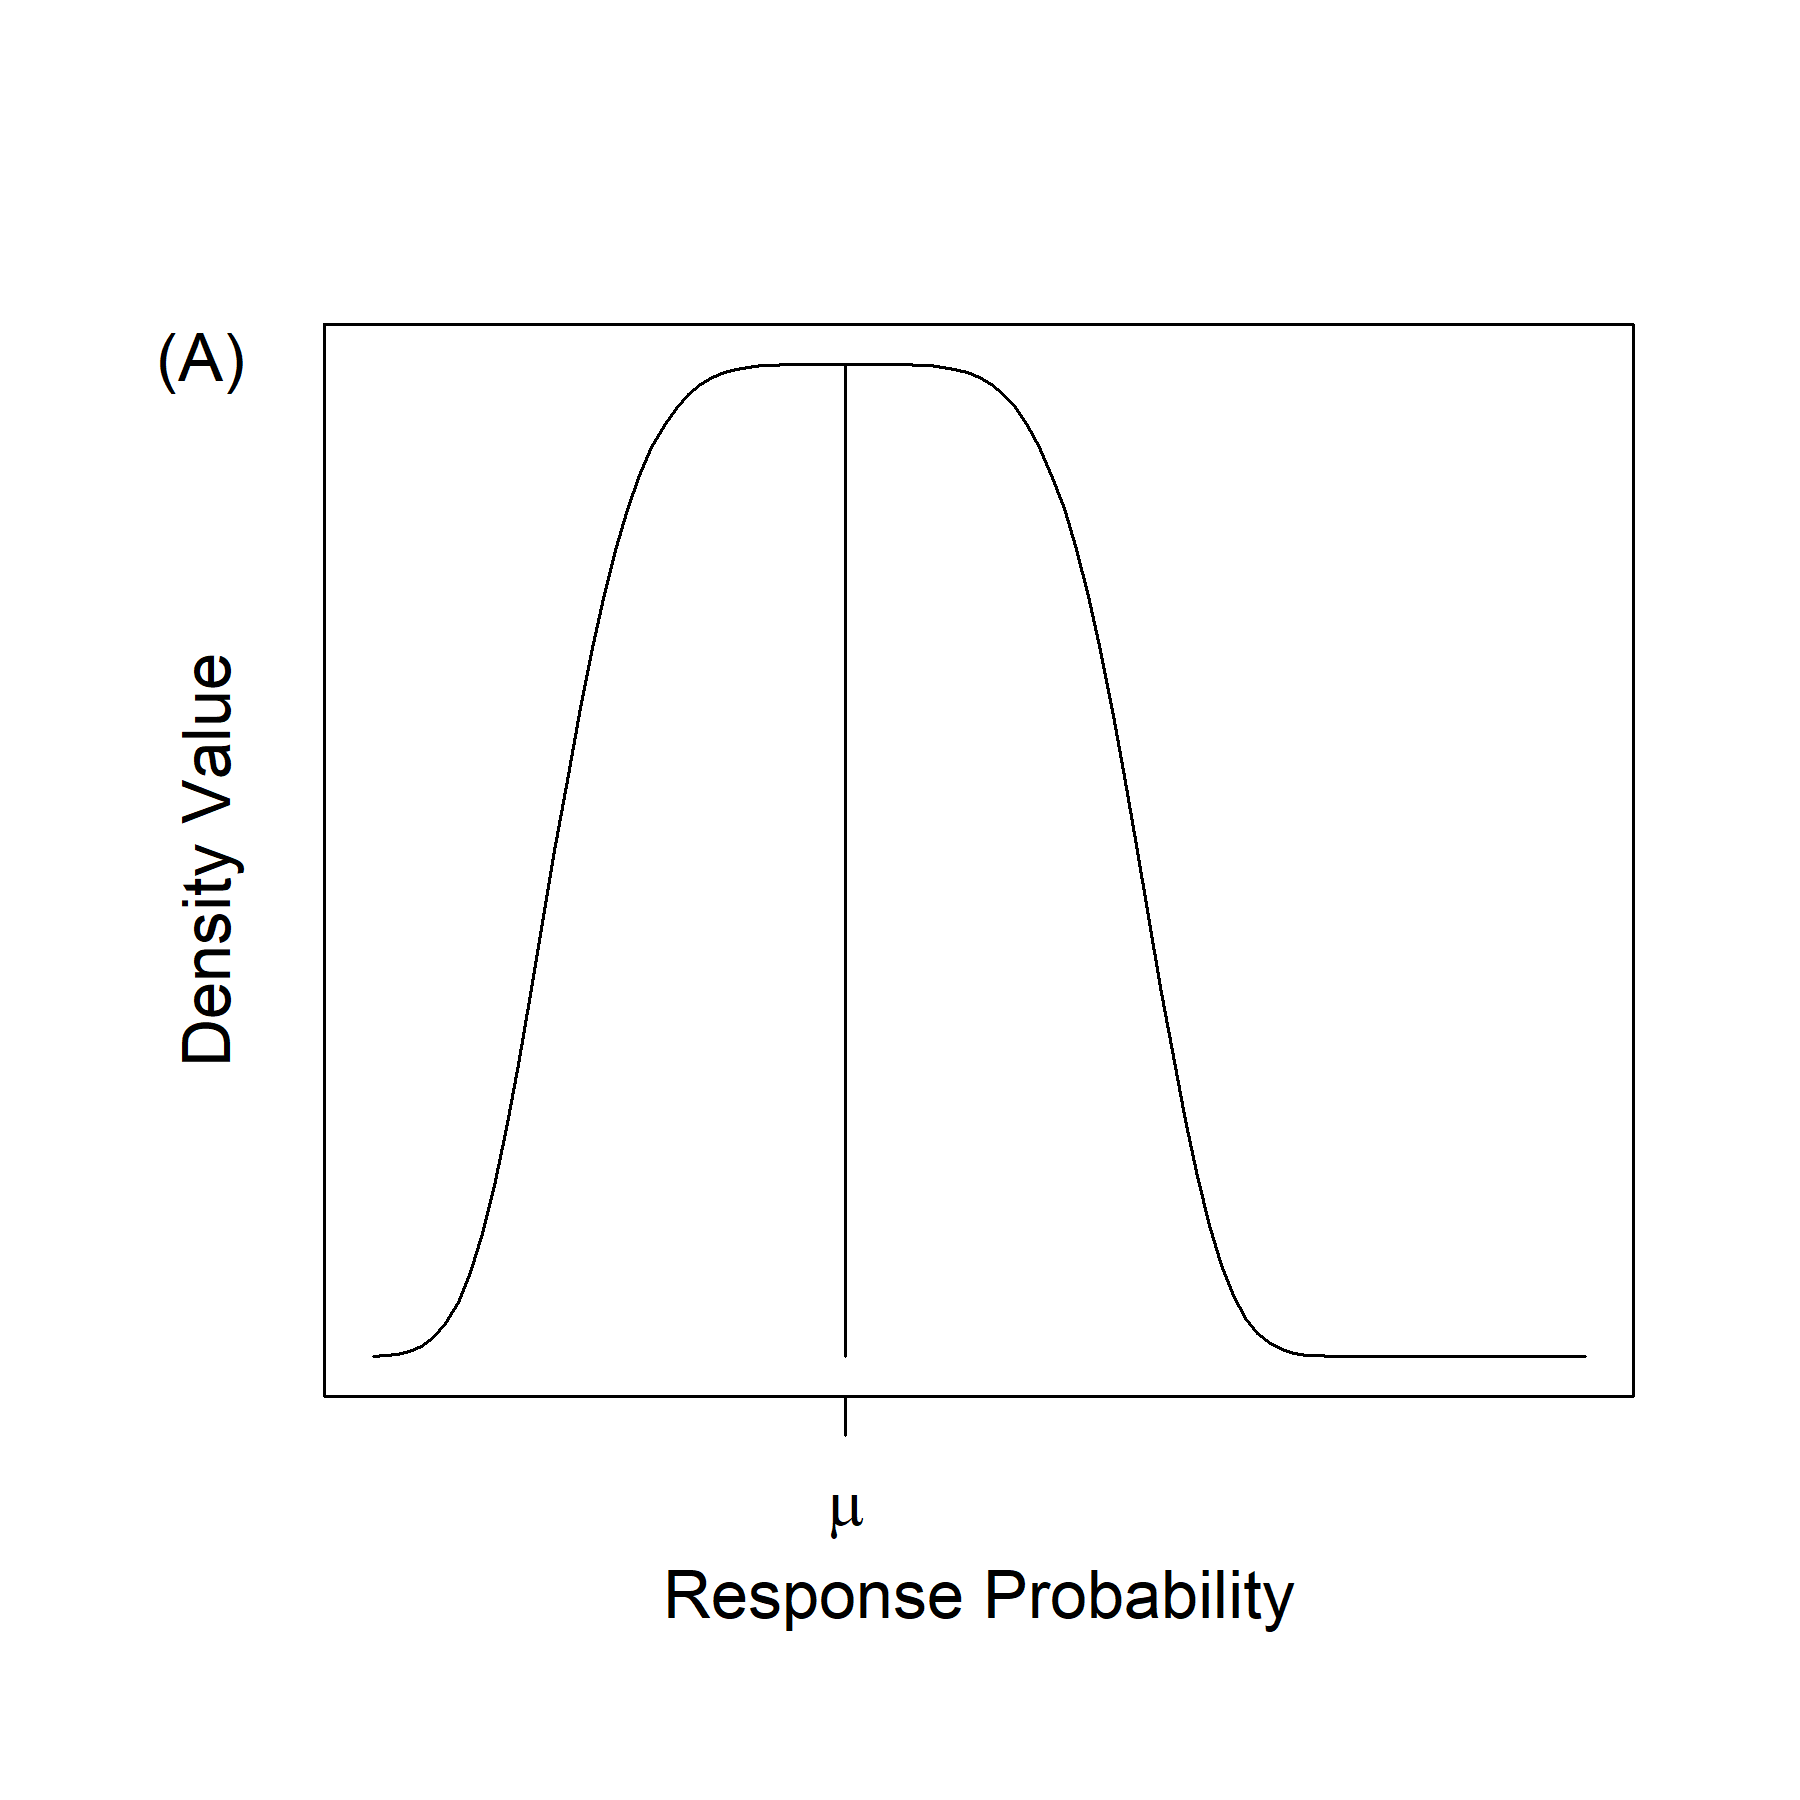
\includegraphics[width=3in]{P:/Bayesian-Sequential-Monitoring/00-paper/FIGURES/figure5c.png}

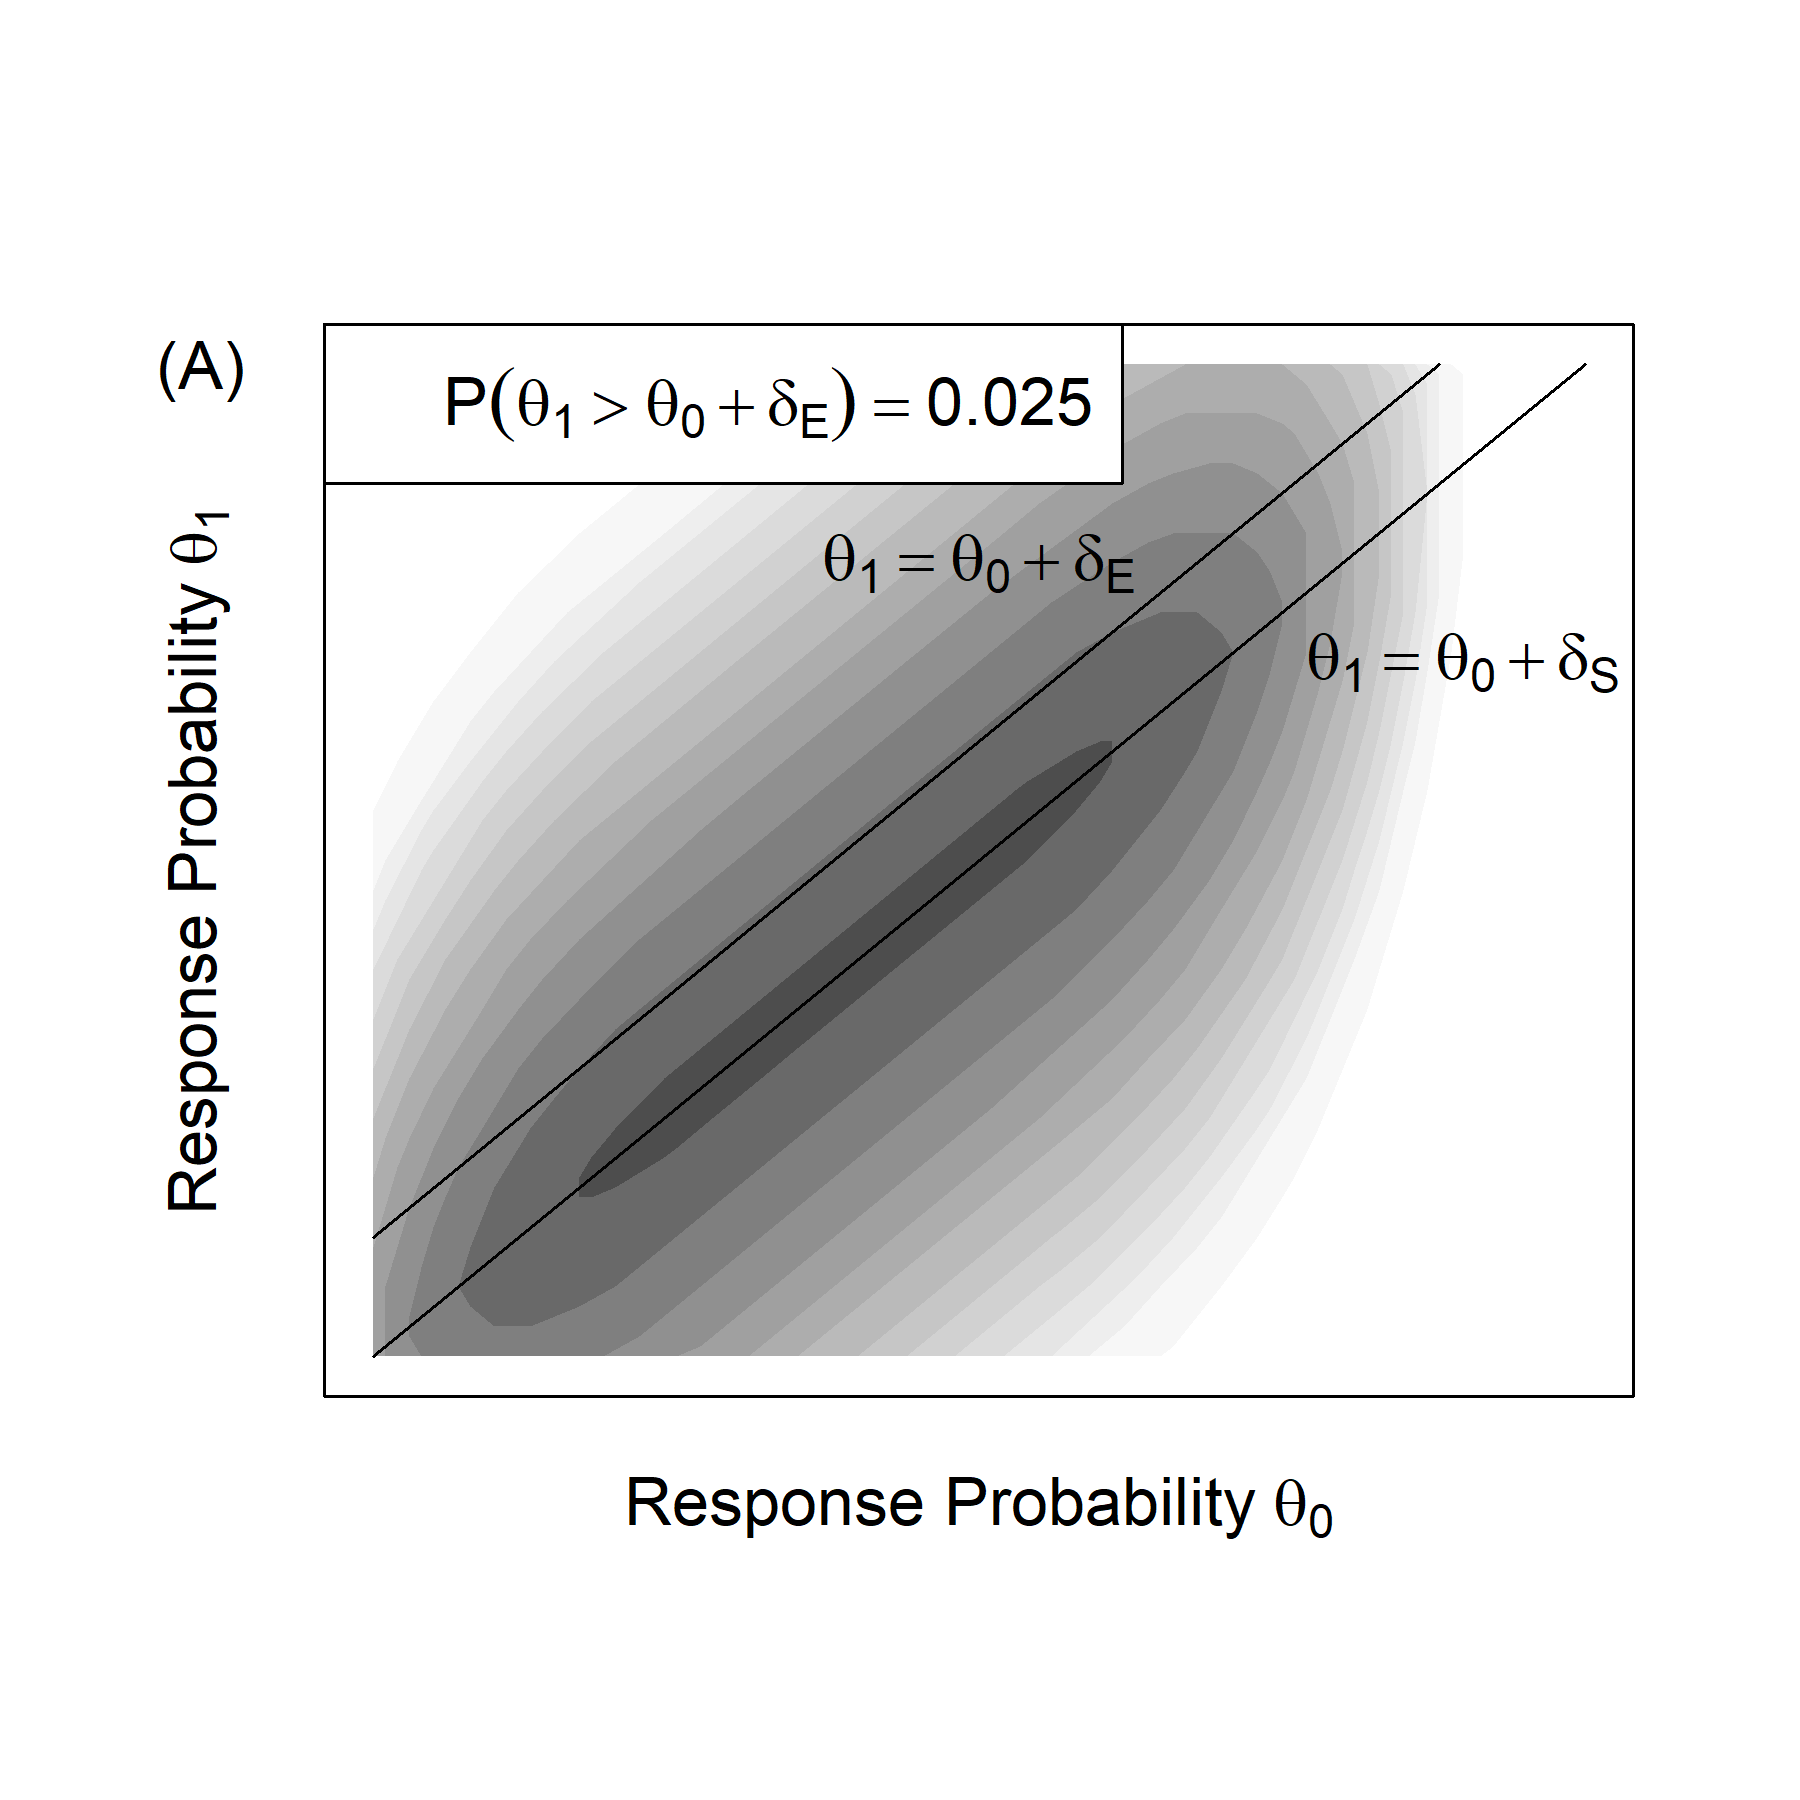
\includegraphics[width=3in]{P:/Bayesian-Sequential-Monitoring/00-paper/FIGURES/figure5a.png}
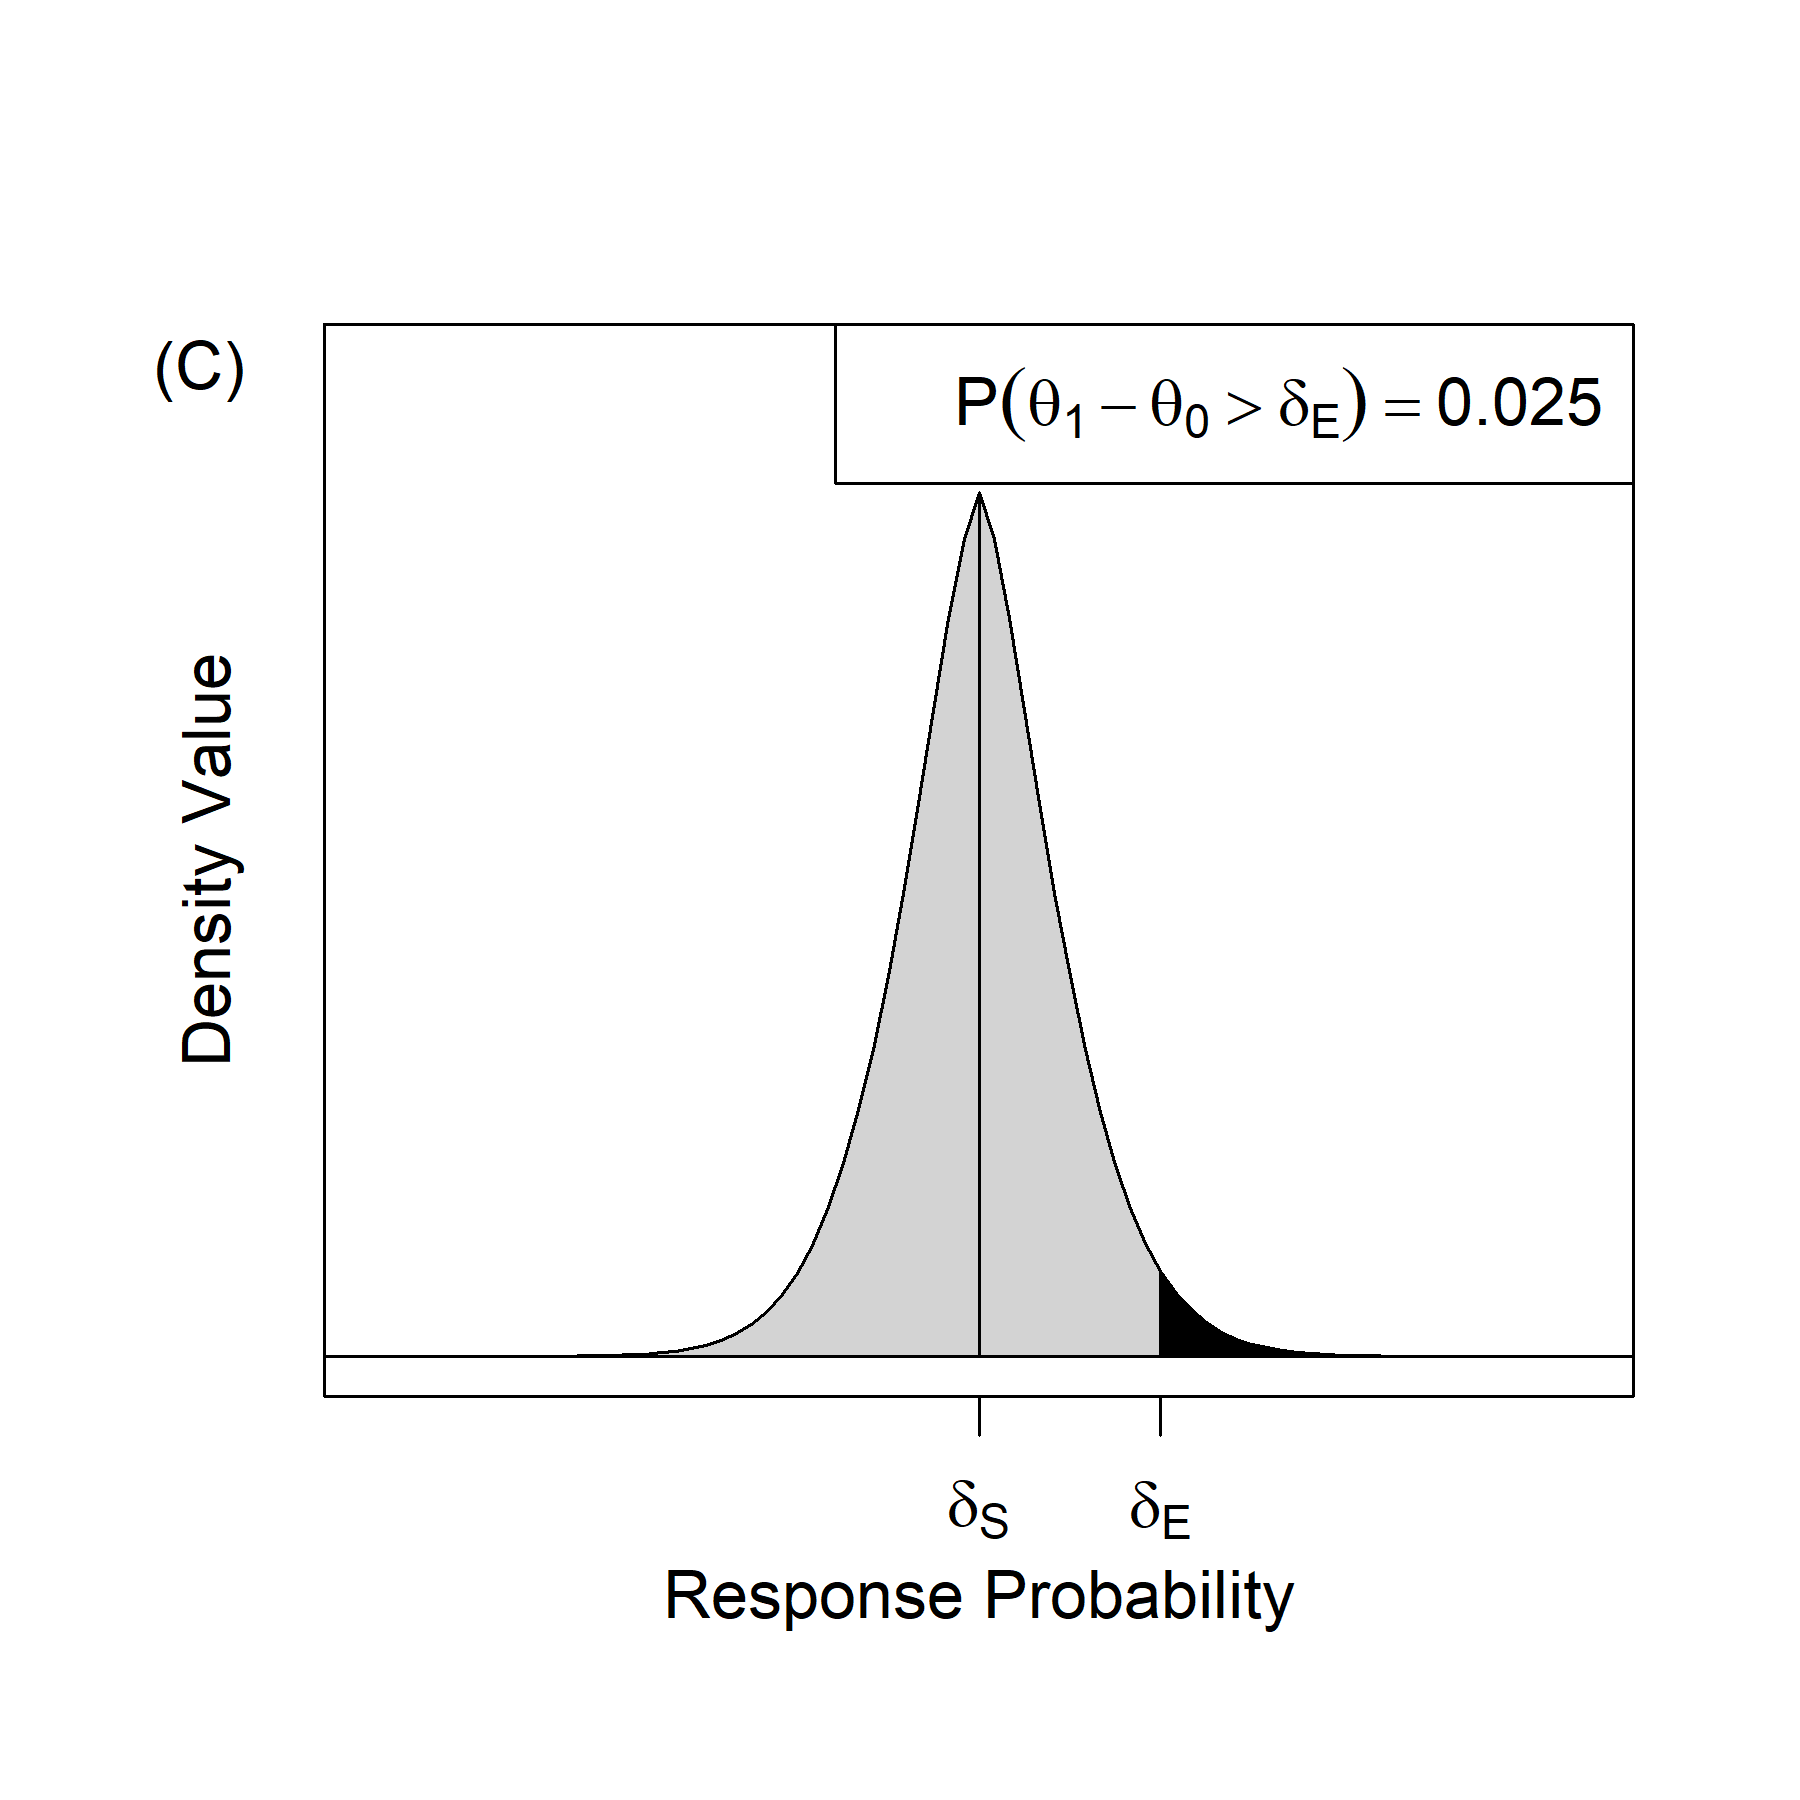
\includegraphics[width=3in]{P:/Bayesian-Sequential-Monitoring/00-paper/FIGURES/figure5d.png}

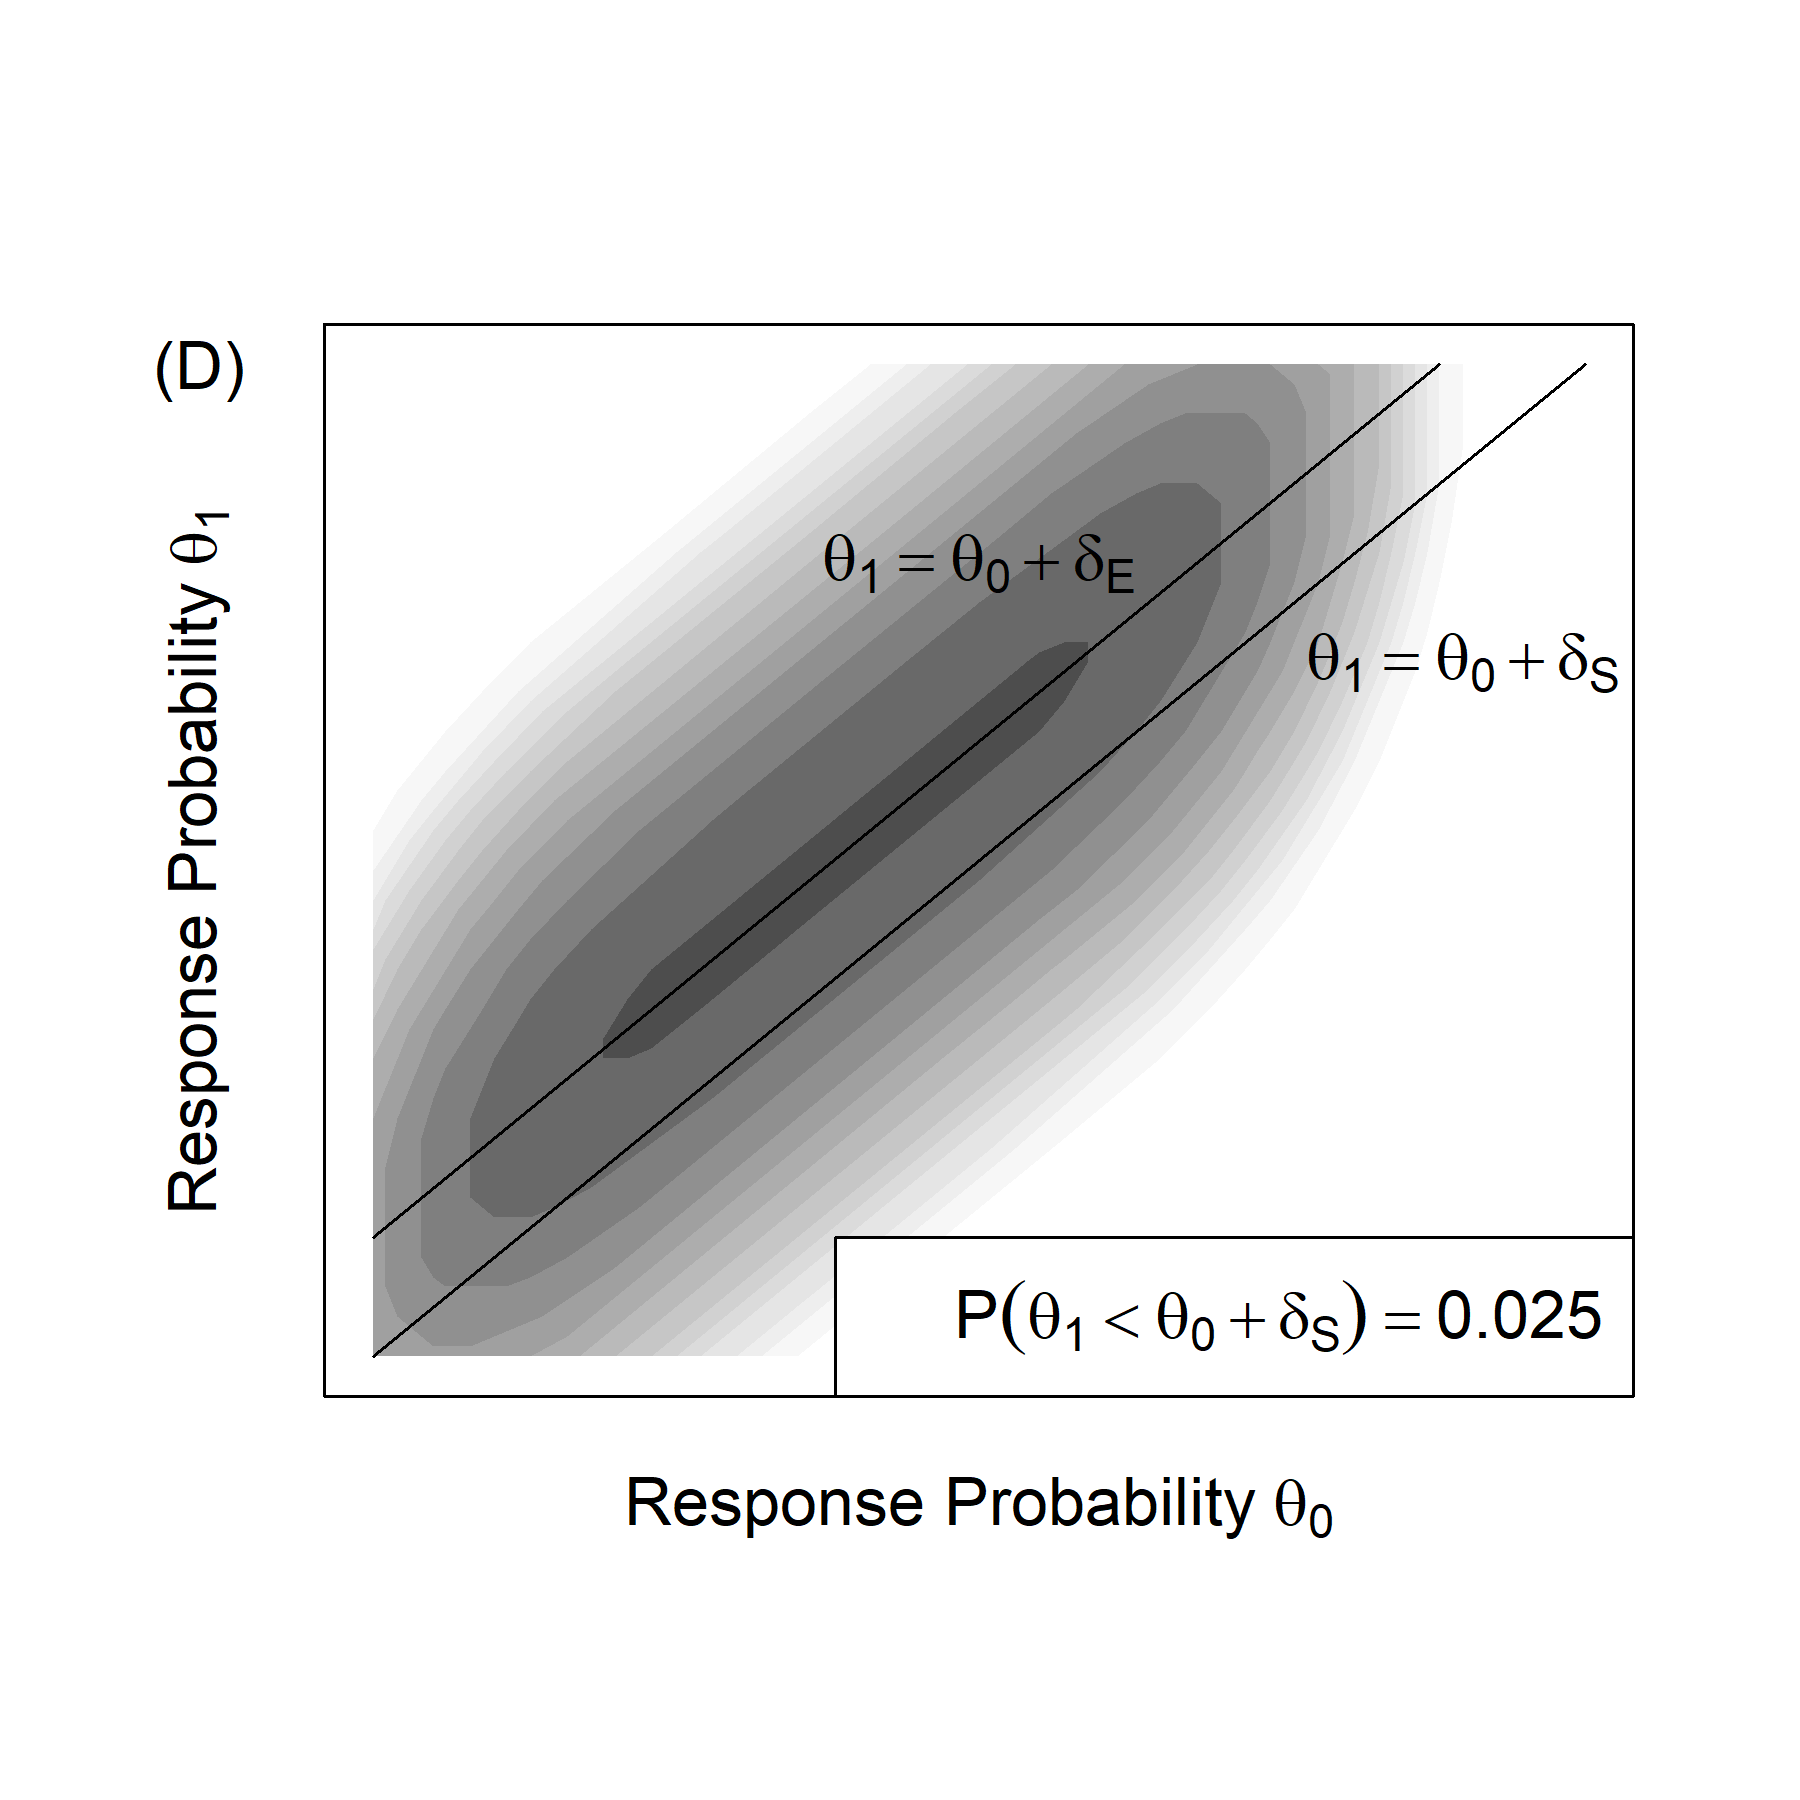
\includegraphics[width=3in]{P:/Bayesian-Sequential-Monitoring/00-paper/FIGURES/figure5b.png}
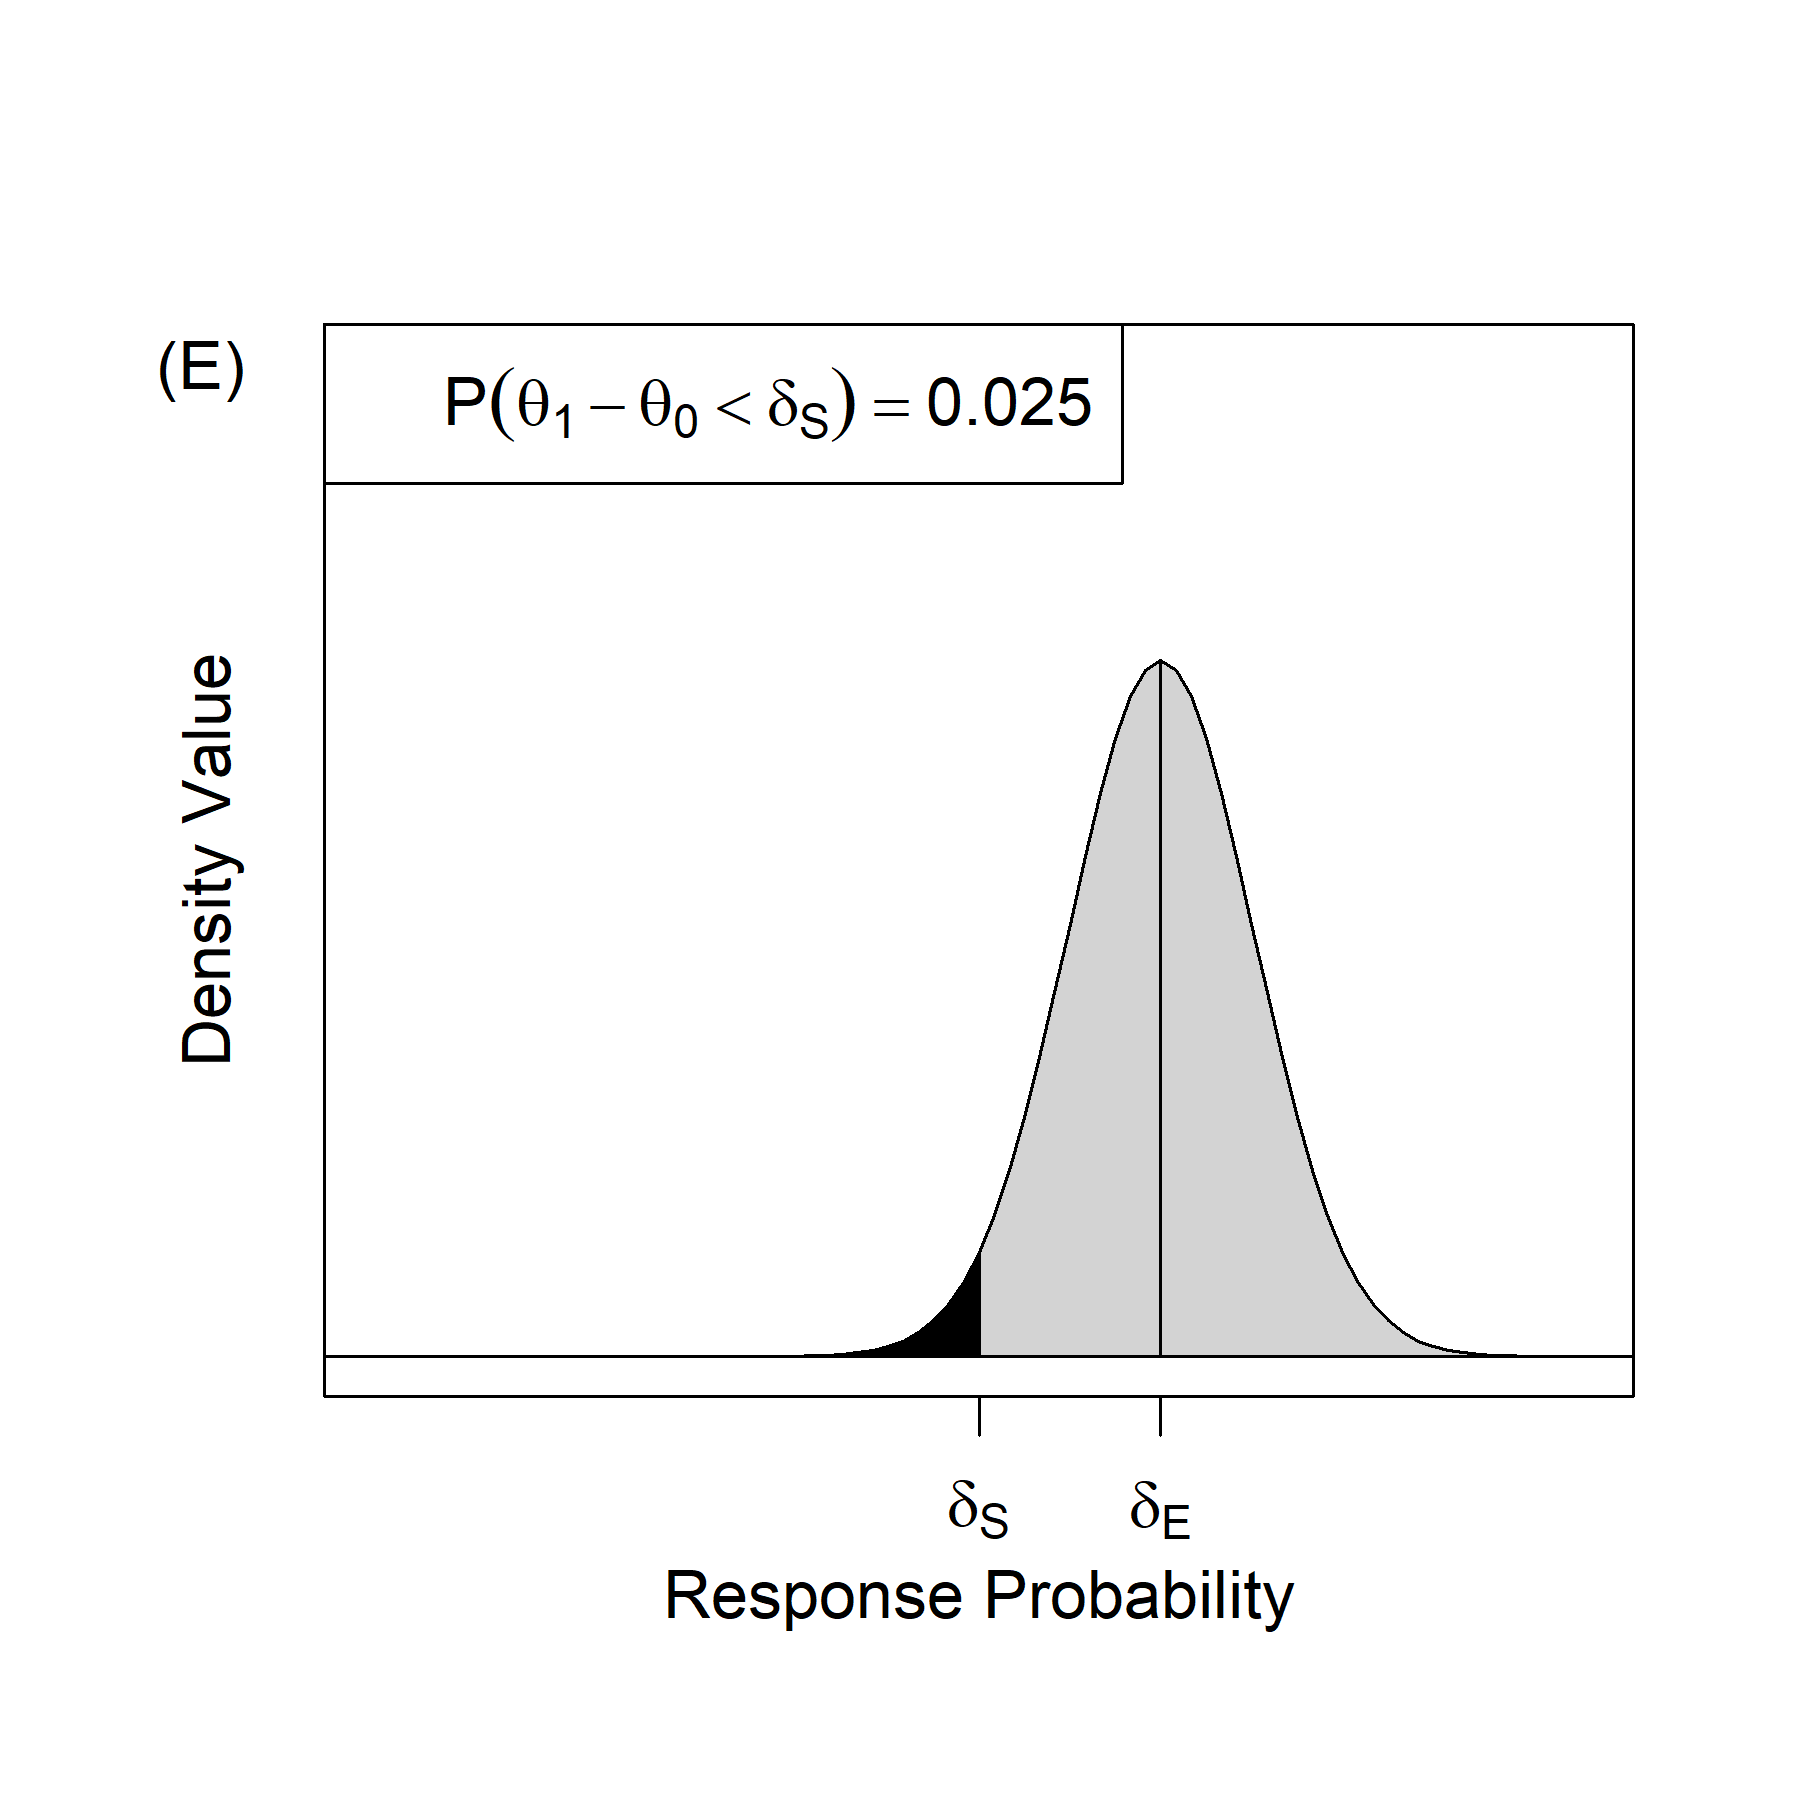
\includegraphics[width=3in]{P:/Bayesian-Sequential-Monitoring/00-paper/FIGURES/figure5e.png}
\caption{A, Univariate prior $\pi(\theta_0)$. B, Skeptical joint prior $\pi_S(\theta_0,\theta_1)$. C, Skeptical marginal prior $\pi_S(\theta_1-\theta_0$. D, Enthusiastic joint prior $\pi_E(\theta_0,\theta_1)$. E, Enthusiastic marginal prior $\pi_E(\theta_1-\theta_0$).}
\label{fig:figure5}
 \end{center}\end{figure}
\subsection{Mixture Inference Priors}
\subsubsection{Definition}
The purpose of the inference prior is to synthesize the posterior inferences from the a priori diverse perspectives to facilitate interpretation of the data once it has been obtained. In this paper we propose using an inference prior that is a combination of the skeptical and enthusiastic priors that were used for monitoring.

The skeptical and enthusiastic monitoring priors defined in Section~\ref{sec:MP} represent extreme but plausible beliefs about $\theta$.
%
While analysis with these priors provides a rational perspective from which one can determine whether interim data are sufficient 
to cease enrolling patients, the a priori belief of most stakeholders will likely fall somewhere in between.
%
Thus, when it interpreting the final data once in hand, intermediate perspectives should be considered.
%
To that end, we define an inference prior as a mixture prior constructed by mixing the monitoring priors.
%
Formally, the inference prior associated with mixing weight $\omega$ is given by
\begin{align}\label{eq:inference_prior}
\pi_{I}\left(\theta\right)=\omega\cdot\pi_{S}\left(\theta\right)+(1-\omega) \cdot \pi_E\left(\theta\right),
\end{align}
where $\omega\in[0,1]$. 
%
The specification of $\omega$ is done a priori, and the value $\omega=1/2$ will be referred to as an agnostic inference prior since it gives equal weight to the skeptical and enthusiastic prior.
%
%\textcolor{green}{
%If I'm not mistaken $\omega_0$ might be a better label for the prior mixing weight and then you could use $\omega\left(\mathbf{D}\right)$ in the expression
%below to represent the posterior mixing weight (which will depend on marginal likelihoods under the two priors). 
%%
%The notation $p(\pi_S|\mathbf{D})$ is not well-defined and will be confusing to reviewers. In my proposal you would use $\omega_0$.
%}
%%
%In particular,
%\begin{align}\label{eq:omega_formula}
%\omega=p(\pi_S|\mathbf{D})=\frac{p(\mathbf{D}|\pi_S)p(\pi_S)}{p(\mathbf{D}|\pi_S)p(\pi_S)+p(\mathbf{D}|\pi_E)p(\pi_E)}
%\end{align}
%where $p(\pi_S)+p(\pi_E)=1$. 
%%
%The quantities $p(\pi_E)$ and $p(\pi_S)$ reflect prior belief in the distribution of $\theta$. 
%%
%A default option is $p(\pi_S)=p(\pi_E)=\frac{1}{2}$. 

The distribution of $\theta$ using the inference 
prior, $p(\theta|\mathbf{D},\pi_I)$, will be used to compute summaries of $\theta$ such as the posterior mean and quantiles. The posterior distribution for $\theta$ using (\ref{eq:inference_prior}) is
\begin{align}
p(\theta|\mathbf{D},\pi_I)&=\hat{\omega}\cdot p(\theta|\mathbf{D},\pi_S)+(1-\hat{\omega})\cdot p(\theta|\mathbf{D},\pi_E)
\end{align}
where the updated mixing weight is
\begin{align}
\hat{\omega}&=\frac{\omega\cdot p(\mathbf{D}|\pi_S)}{\omega\cdot p(\mathbf{D}|\pi_S)+(1-\omega)\cdot p(\mathbf{D}|\pi_E)}
\end{align}
where $p(\mathbf{D}|\pi_S)=\int p(\mathbf{D}|\theta)\pi_S(\theta)d\theta$ and $p(\mathbf{D}|\pi_E)=\int p(\mathbf{D}|\theta)\pi_S(\theta)d\theta$. 

%
%Choosing $\omega=1/2$ for an equal mixture of $\pi_S$ and $\pi_E$ corresponds to an inference prior that equally weights the skeptical and enthusiastic opinions. Define $p(\mathbf{D}|\pi(\theta))=\int p(\mathbf{D}|\theta)\pi(\theta)d\theta$ to be the marginal likelihood for the data given the prior $\pi(\theta)$. Choosing $\omega$ based on posterior model probabilities of the null and alternative hypotheses yields 
%\begin{align}
%\omega=\frac{p(\mathbf{D}| \pi_{S})}{p(\mathbf{D}| \pi_{S})+p(\mathbf{D}| \pi_{E})}. 
%\end{align}
%The determination of a significant trial result is given by
%\begin{align*}
%P(\theta\in\Theta_1|\mathbf{D},\pi_I)\geq\delta.
%\end{align*} 

%All relevant information about $\theta$ can be derived from the marginal posterior distribution with an inference prior (e.g. posterior mean, credible intervals). For example, the posterior mean using the inference prior will be a two-part mixture of the posterior means using the skeptical and enthusiastic priors: $E(\theta|\mathbf{D},\pi_I)=\omega E(\theta|\mathbf{D}, \pi_{S})+(1-\omega) E(\theta|\mathbf{D}, \pi_{E}).$
\subsubsection{Incorporating Prior Information in the Monitoring Priors}
The skeptical and enthusiastic monitoring priors can be viewed as a weighted combination such as in the inference prior (\ref{eq:inference_prior}) with weights $\omega=1$ and $\omega=0$ respectively. This weighted combination can be used as a replacement for the monitoring prior for any fixed weight $\omega$. For example, a ``not-as-skeptical" prior can be defined as $\tilde{\pi_S}(\theta)=0.75\cdot\pi_S(\theta)+0.25\cdot\pi_E(\theta)$. 

Alternatively, $\omega$ can be informed by the data. Let $\hat{\theta}=argmax \{p(\mathbf{D}|\theta)\}$ be the maximum likelihood estimator of $\theta$ given the data. Define
\begin{align}
\omega=\frac{\pi_S(\hat{\theta})}{\pi_S(\hat{\theta})+\pi_E(\hat{\theta})}
\end{align}
as a mixing weight that dynamically gives preference to the prior that has the higher density evaluated at $\hat{\theta}$.
%\textcolor{green}{We don't have anything in the paper about using a mixture of the skeptical and enthusiastic prior to 
%define a ``less'' skeptical monitor prior that incorporates information from another source using the 
%notion of applicability (i.e., a fixed value of $\omega_0$ that is not 1.). 
%%
%This is fundamental to the novelty of the paper. 
%%
%I think it would be good to show how the GN can be used to inform a prior for the control group with flexibility here (e.g., flattening the prior over an interval)
%AND talking about the mixture skeptical monitoring prior.
%%
%In the case of using ``no prior information'' the enthusiastic prior is simply used for monitoring. But it can be incorporated directly into the 
%skeptical prior when it is informed by data using the concept of applicability.
%%
%Isn't that what was done for the second example? Lets talk if we need to. This is a big part of the novelty.
%}

%\\
%\int_\Theta \theta p(\theta|\mathbf{D},\pi_{I})d\theta&=\omega\cdot \int_\Theta \theta p(\theta|\mathbf{D},\pi_{S})d\theta+(1-\omega)\cdot\int_\Theta \theta %p(\theta|\mathbf{D},\pi_{E})d\theta
%\begin{align*}
%\pi_{Inference}=\frac{p(\mathbf{D}| \pi_{S}) \pi_{S}+p(\mathbf{D}| \pi_{E}) \pi_{E}}{p(\mathbf{D}| \pi_{S})+p(\mathbf{D}| \pi_{E})}
%\end{align*}
%\begin{align*}
%E(\theta|\mathbf{D},\pi_{Inference})=\omega\times E(\theta|\mathbf{D}, \pi_{S})+(1-\omega)\times E(\theta|\mathbf{D}, \pi_{E})
%\end{align*}
%Need to describe relation to Type I and Type II error.
%\subsubsection{Default parameterization of monitoring priors for common designs}\label{monitoring_prior_specification}
%Define prior distribution as $\pi(\theta|\lambda)$ where $\lambda$ is a vector of hyperparameters.

%Reference prior attempts to express no particular opinion about the treatment's merit. 

\section{Examples}\label{sec:examples}

\subsection{Single-Arm Proof-of-Activity Trial with Binary Endpoint}\label{sec:example1}
\subsubsection{Motivating example}
Consider the T72 pediatric trial ``A Study of the Safety and Efficacy of Infliximab (REMICADE) in Pediatric Patients With Moderately to Severely Active Ulcerative Colitis" (NCT00336492) ~\cite{Hyams2012}. Infliximab was given to all subjects at the 5mg/kg dose at weeks 0, 2, and 6, and the primary end point was response at week 8. Response was measured by improvement in disease severity scores.

The initial enrollment occurred on August 25, 2006, and the last assessment was June 24, 2010. If the patient showed improvement at week 8 then they continued treatment and would have their last assessment at week 54. The response rate at 8 weeks was $73.3\%$ $(N=60)$, so it is likely that the last assessment was at week 54, and we can infer enrollment took place over approximately 33.5 months (approximately 1 enrollment per 17 days). 

The sample size of $60$ patients was chosen to ensure $12\%$ precision in estimating the true response proportion with at $95\%$ CI, assuming a response rate of $67\%$ as was observed among adults from the ACT 1 and ACT 2 trials ~\cite{Rutgeerts2005} at the same 5mg/kg dose $(N=242)$. A $95\%$ confidence interval that excluded $0.40$ was determined to be a clinically significant result.

\subsubsection{Model formulation \& prior elicitation}
The data $\mathbf{D}$ are assumed to be independent Bernoulli random variables with common response probability $\theta$. The null response value is $\theta_0=0.40$ and a highly efficacious response probability is $\theta_1=0.67$. The hypothesis for this trial is $H_0:\leq \theta_0$ vs $H_1:\theta > \theta_0$.

The default skeptical and enthusiastic priors will be of the form (\ref{eq:generalizednormalkernel}) and are truncated to the unit interval. 
\begin{align}
\pi_S(\theta)&\propto \exp\left\{-\frac{|\theta-\theta_0|}{\alpha_S}^{\beta_S}\right\} I(\theta\in[0,1]) \label{eq:ex1skptprior}\\
\pi_E(\theta)&\propto \exp\left\{-\frac{|\theta-\theta_1|}{\alpha_E}^{\beta_E}\right\} I(\theta\in[0,1])\label{eq:ex1enthprior}
\end{align}

The values $\beta_S$ and $\beta_E$ are pre-specified and $\alpha_S$ and $\alpha_E$ are chosen to satisfy the tail-probability conditions 
(\ref{eq:enthprior})-(\ref{eq:skptprior}).

The skeptical prior is shown in Figure \ref{fig:figure1}(B), which has added concentration around the null response value $\theta_0$ by pre-specifying $\beta_S>2$. The enthusiastic prior is shown in Figure \ref{fig:figure1}(C) with a default choice of $\beta_E=2$. The level of residual uncertainty is given by $\epsilon=0.025$. The skeptical prior was chosen to have additional Type 1 error control. A comparison of the various combinations of the monitoring priors in Figure~\ref{fig:figure1} is provided in Appendix \ref{sec:priorRobustness}.

Enrollment will proceed until one of the following three conditions are satisfied:
\begin{align}
\text{Efficacy criteria (EFF): }&P(\theta>\theta_0|\mathbf{D},\pi_S)\geq 1-\epsilon \label{eq:ex1efficacy}\\
\text{Futility criteria (FUT): }&P\left(\theta\leq\frac{\theta_0+\theta_1}{2} \Big|\mathbf{D},\pi_E\right)\geq 1-\epsilon \label{eq:ex1futility}\\
\text{Maximum sample size: }&N=112 \text{ patient outcomes obtained}\label{eq:ex1maxss}
\end{align}

where the maximum sample size was chosen based on a frequentist design to have $80\%$ power at a true response proportion of $\frac{\theta_0+\theta_1}{2}=0.535$.

If enrollment is terminated due to the efficacy or futility criteria being satisfied, those subjects who are still undergoing follow-up will still have their outcomes considered in the final analysis.

\subsubsection{Example paths}
Violin plots are used to show the results of a simulated trials with the initial prior specification (first panel), three interim analyses (middle panels), and a final analysis (last panel), where interim analyses are conducted after every 10 completed outcomes. The first panel shows the skeptical and enthusiastic prior distributions from (\ref{eq:ex1skptprior}), (\ref{eq:ex1enthprior}), which are the same as introduced in Figure \ref{fig:figure1}(b) and (c). The other panels show the posterior distributions using the skeptical and enthusiastic priors respectively. An inference prior is defined as the mixture (\ref{eq:inference_prior}) with $\omega=0.5$, and its mean and $95\%$ credible intervals are shown.

Figure \ref{fig:figure2}(a) shows the results of a trial where at the third interim analysis the efficacy condition (\ref{eq:ex1efficacy}) is satisfied and enrollment is terminated. Note that in the final analysis the efficacy condition is no longer at the $1-\epsilon$ threshold. A discussion of this type of ``evidence decrease" is given in Section \ref{sec:ex1.1}.

Figure \ref{fig:figure2}(b) shows the results of a trial where at the third interim analysis the futility condition (\ref{eq:ex1futility}) is satisfied and enrollment is terminated. 

\begin{figure}\begin{center}
    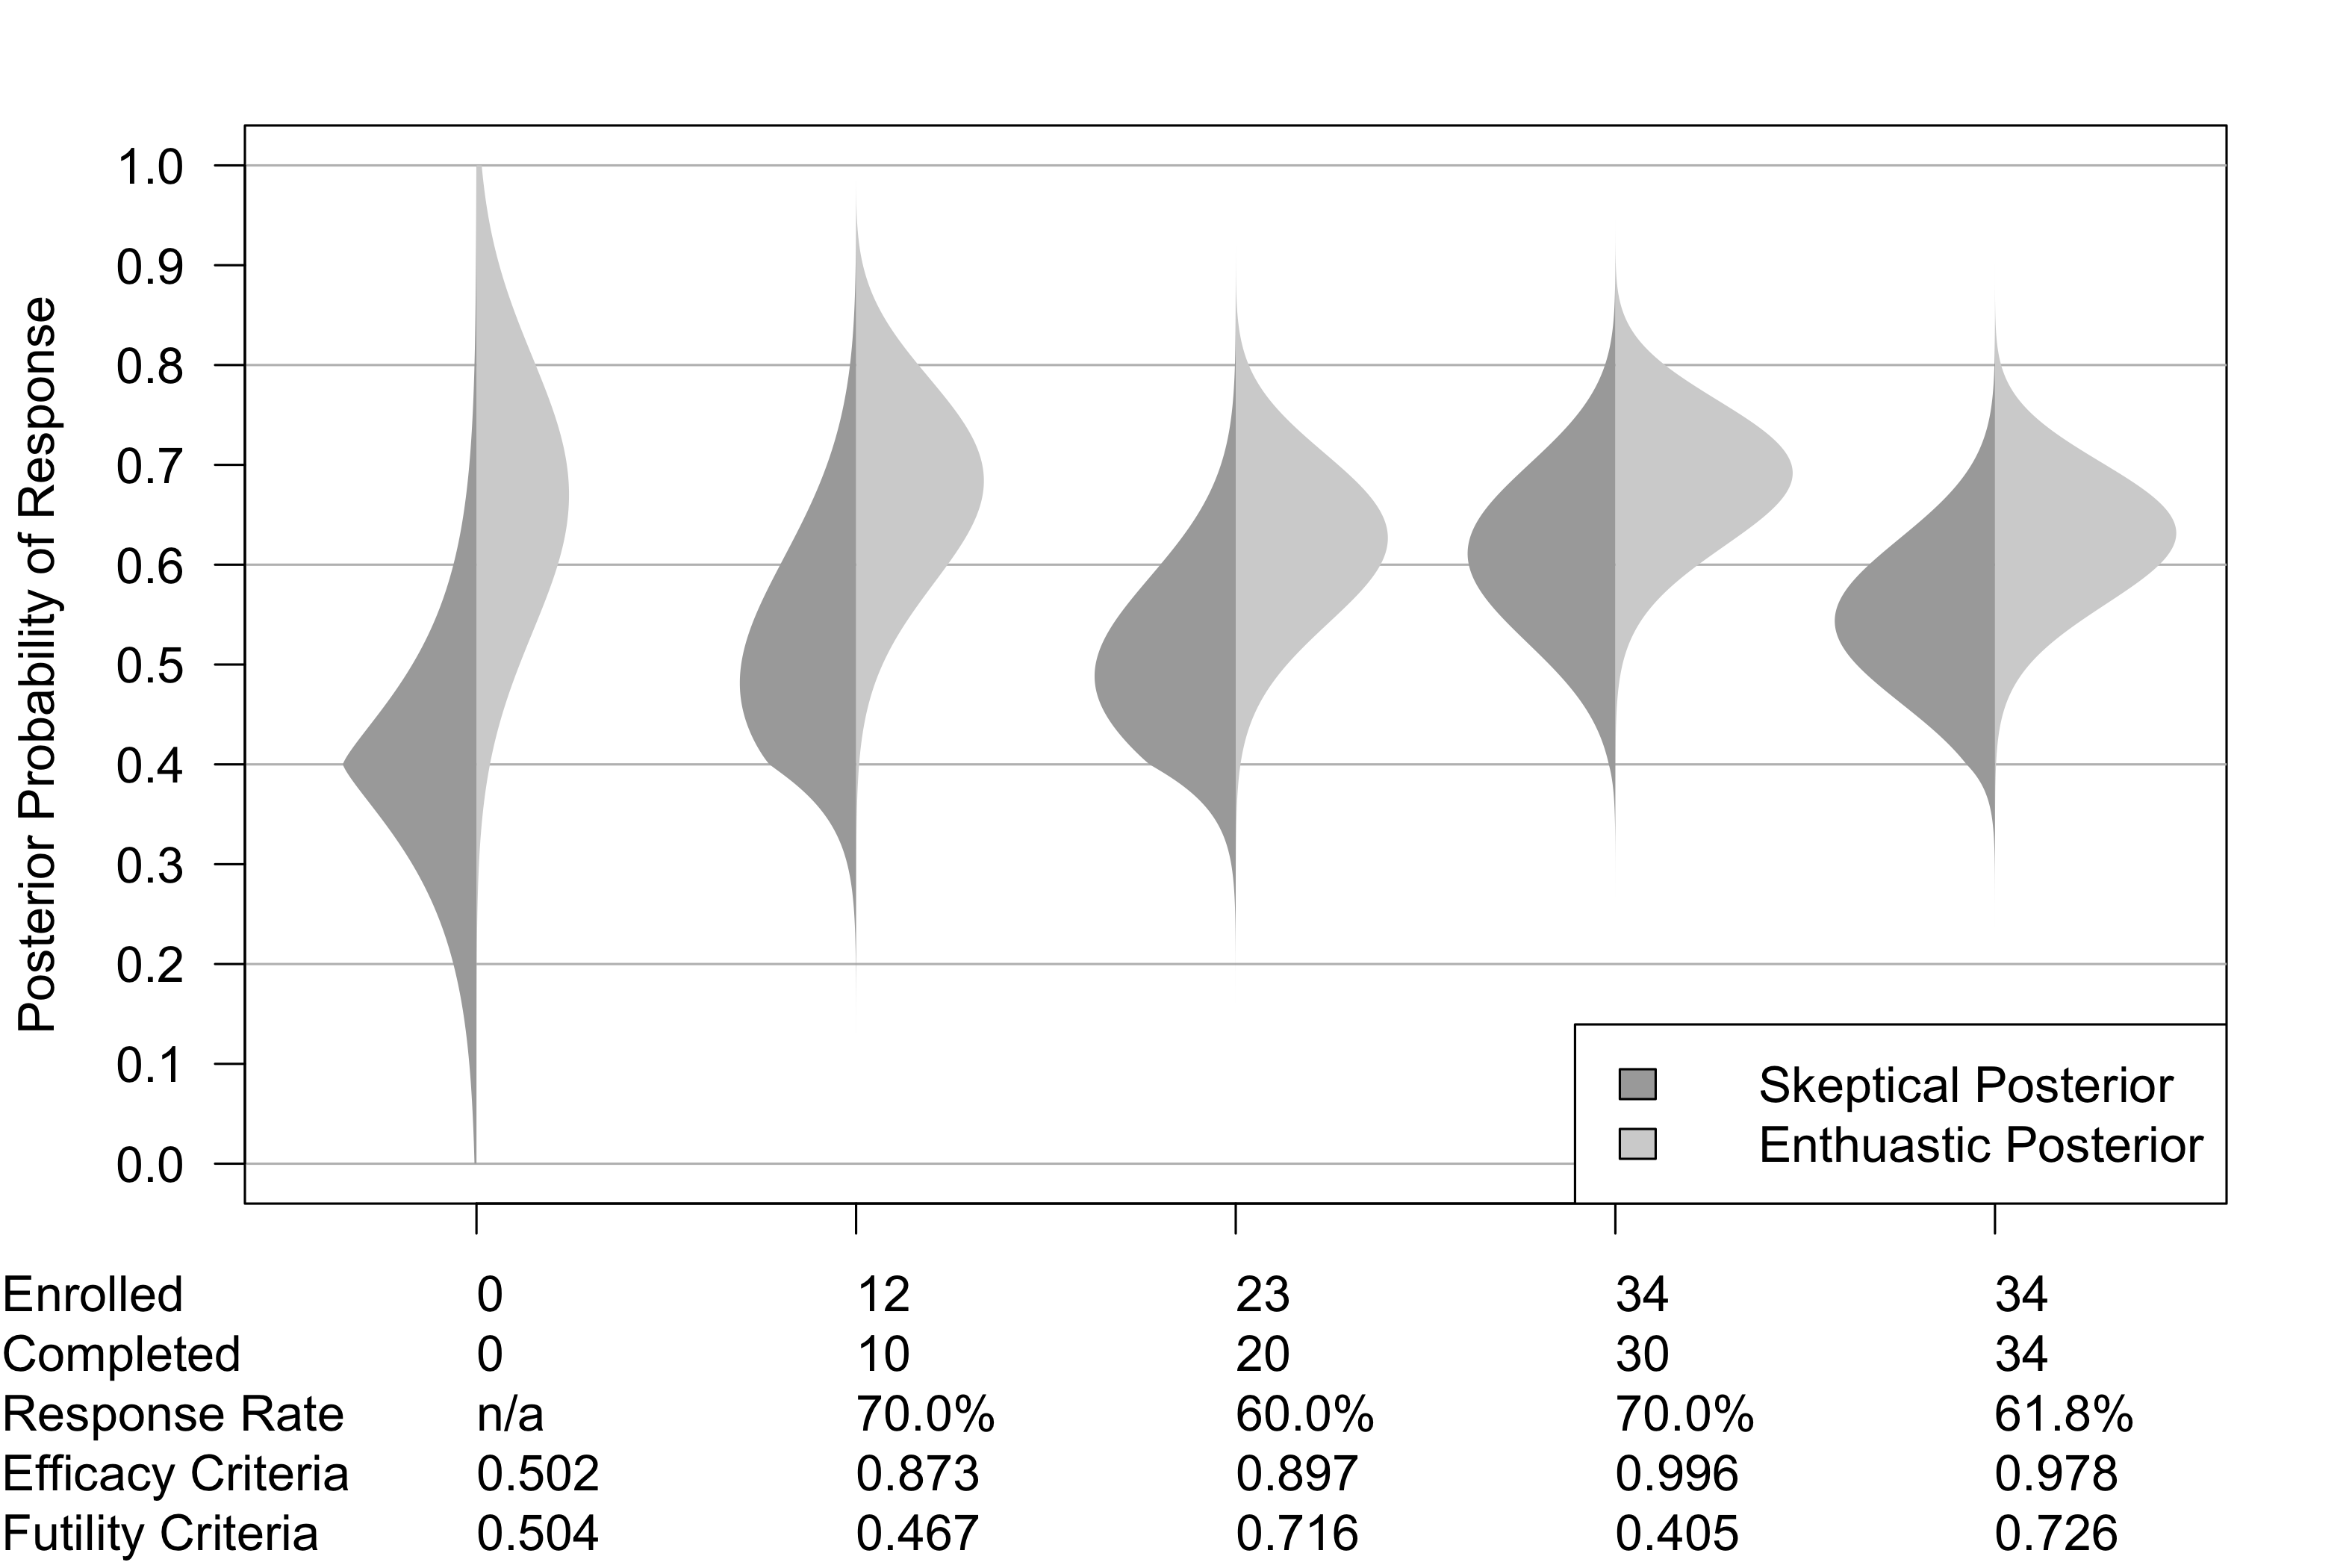
\includegraphics[width=7in]{P:/Bayesian-Sequential-Monitoring/00-paper/FIGURES/figure2a.png}
    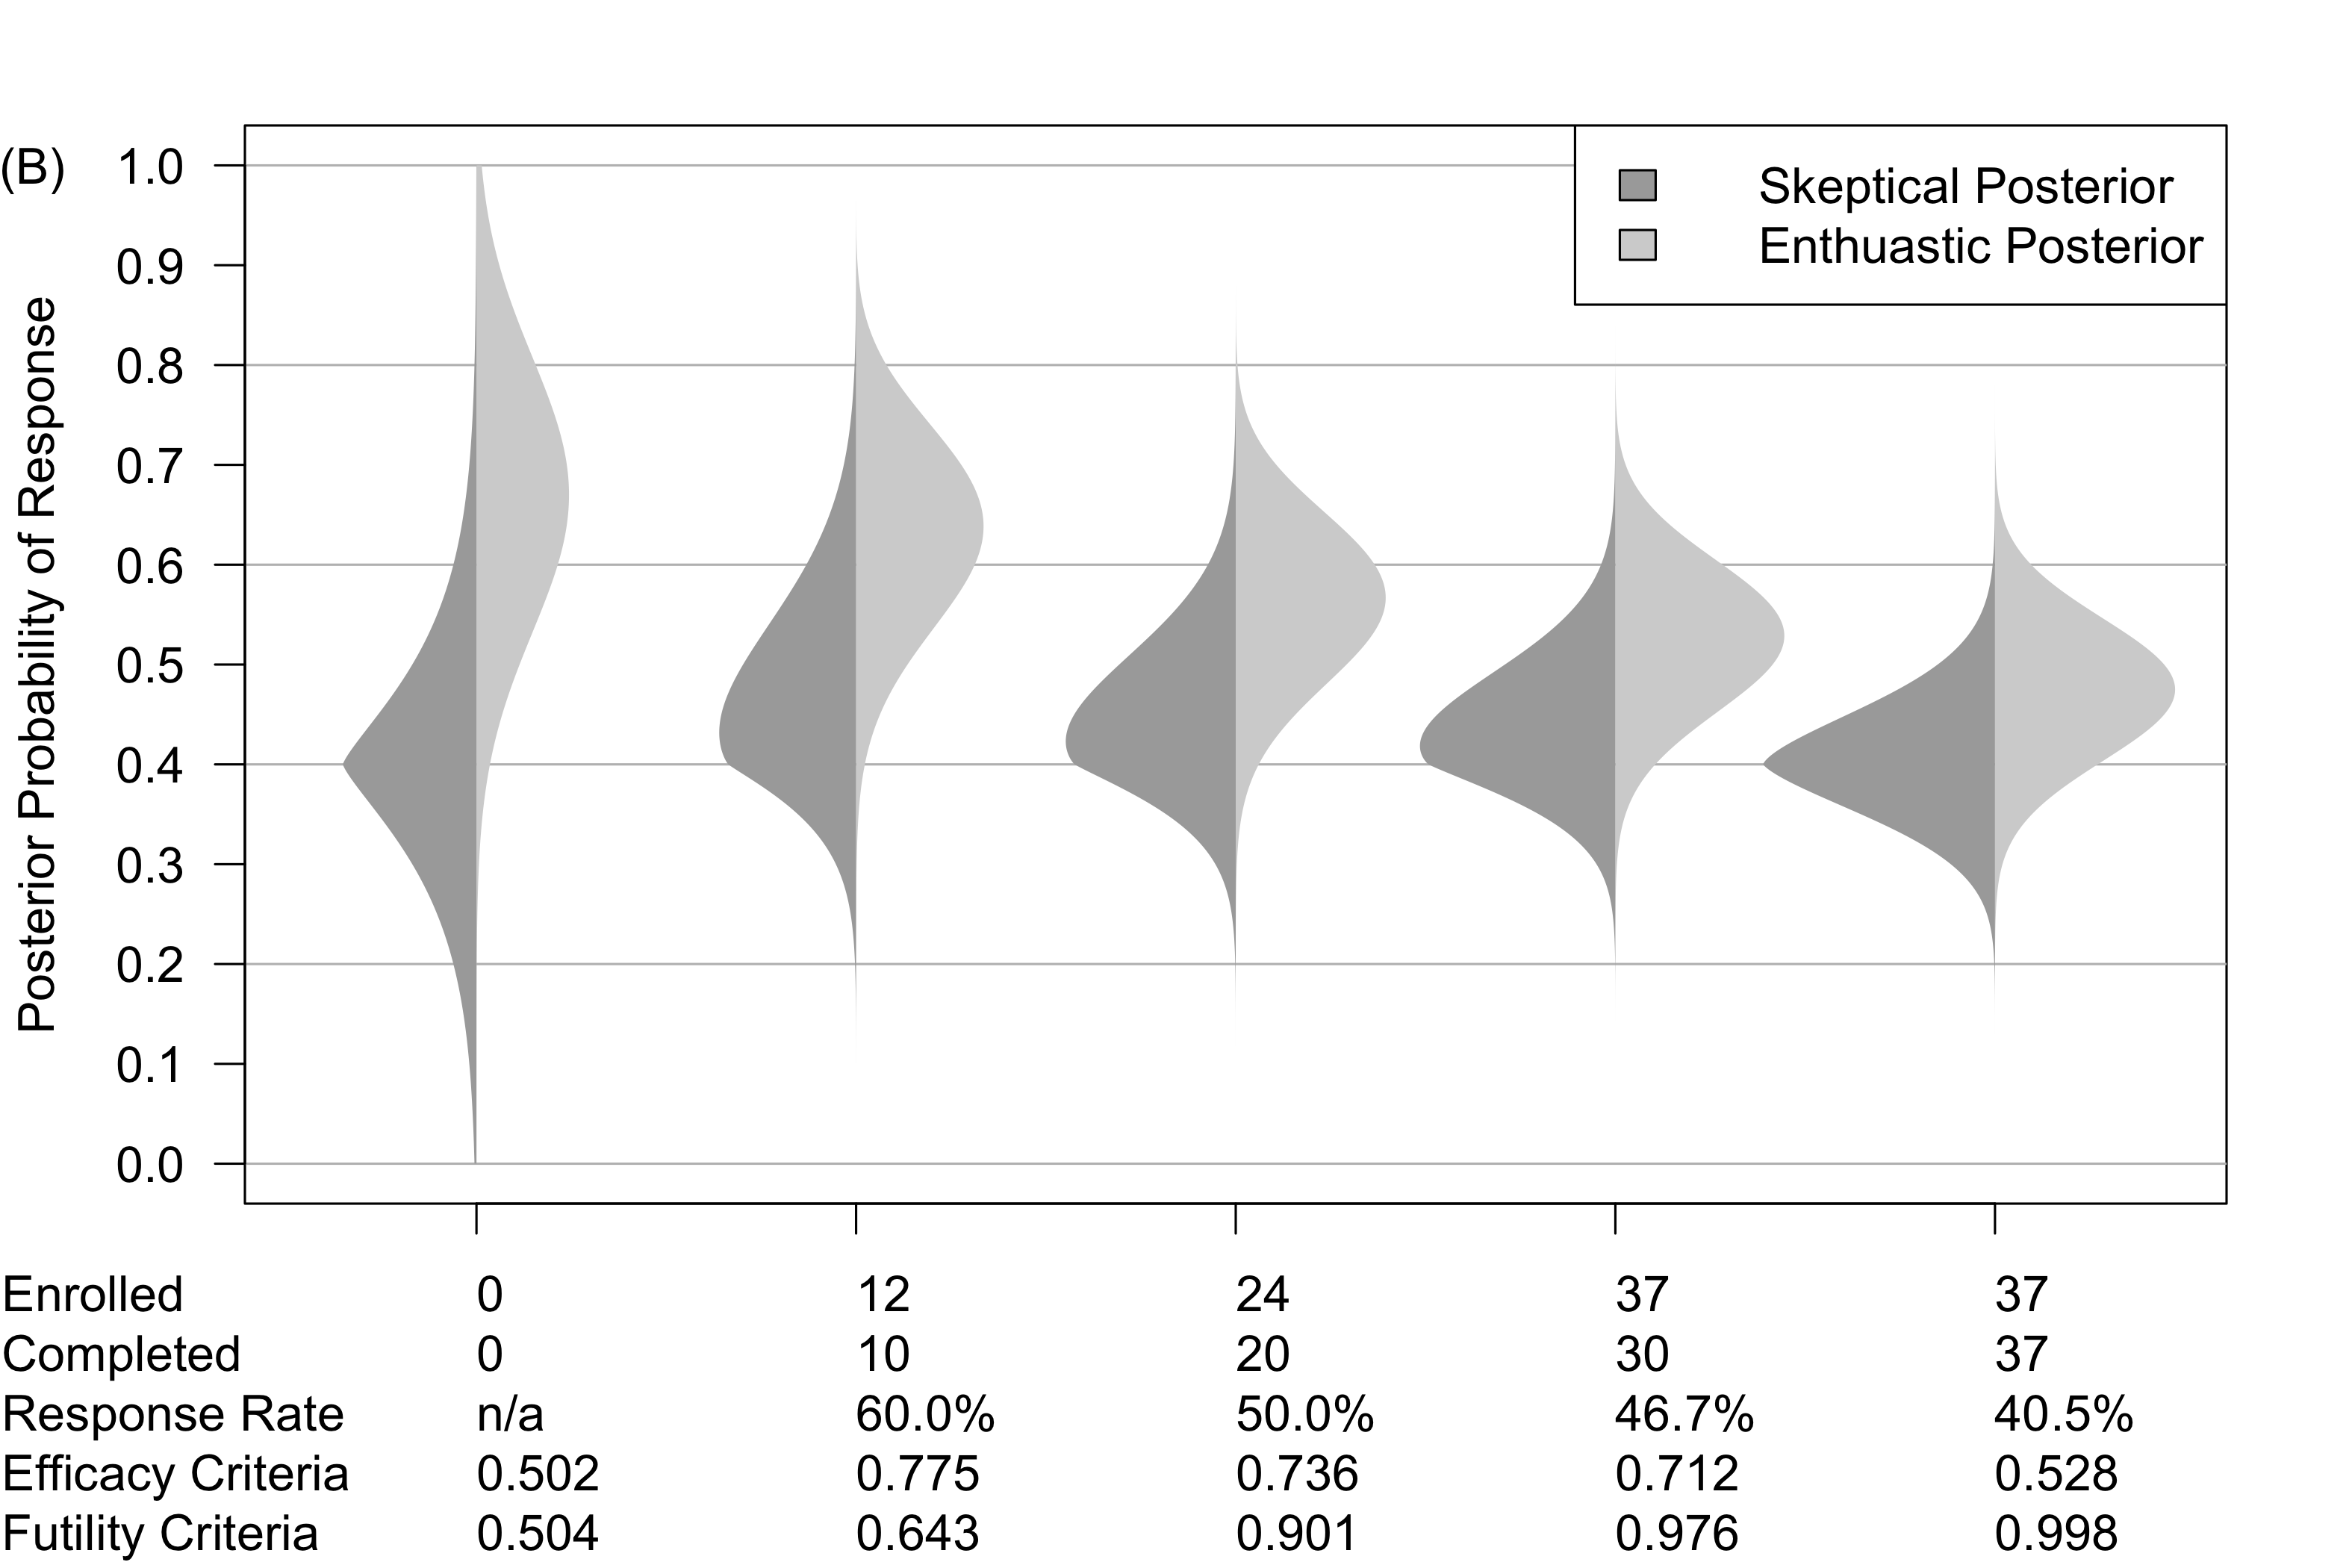
\includegraphics[width=7in]{P:/Bayesian-Sequential-Monitoring/00-paper/FIGURES/figure2b.png}
    \caption{A, Early stoppage for efficacy. B, early stoppage for futility.}
	\label{fig:figure2}

 
\end{center}\end{figure}
\subsubsection{Preposterior Analysis of Operating Characteristics}\label{sec:ex1.1}
An interim analysis will be completed after every 2 subjects complete follow-up. The inference prior is defined as the mixture (\ref{eq:inference_prior}) with $\omega=0.5$ is used in evaluating the posterior mean and coverage probability.

Figure \ref{fig:ex1.1} shows the operating characters of this particular trial design. Stopping early for efficacy refers to satisfying (\ref{eq:ex1efficacy}), stopping early for futility refers to satisfying (\ref{eq:ex1futility}), and inconclusive findings refers to (\ref{eq:ex1maxss}). 

When the true response probability is $\theta=\theta_0$, there is a $3.9\%$ probability of stopping the trial early for efficacy. The posterior mean shows a slight bias towards the alternative hypothesis.

Figure \ref{fig:ex1.1} addresses the particular situation of when the efficacy criteria (\ref{eq:ex1efficacy}) is satisfied at an interim analysis triggering termination of enrollment of additional subjects, but once the outcomes of subjects undergoing follow-up are ascertained the criteria is no longer satisfied. The distribution of the efficacy criteria given the final data for these cases are shown. The probability of these cases occurring is reflected by the percent agreement between interim and final results, and it is shown that as $\theta$ increases there is a higher probability of agreement and therefore a lower probability of evidence decrease.

The median efficacy criteria is very close to $1-\epsilon$ and in the vast majority of cases (greater than 10th percentile) the efficacy criteria is still very high. Therefore, for this trial design, the interim and final results are not highly discrepant with respect to the efficacy criteria in these cases.
\begin{figure}\begin{center}

    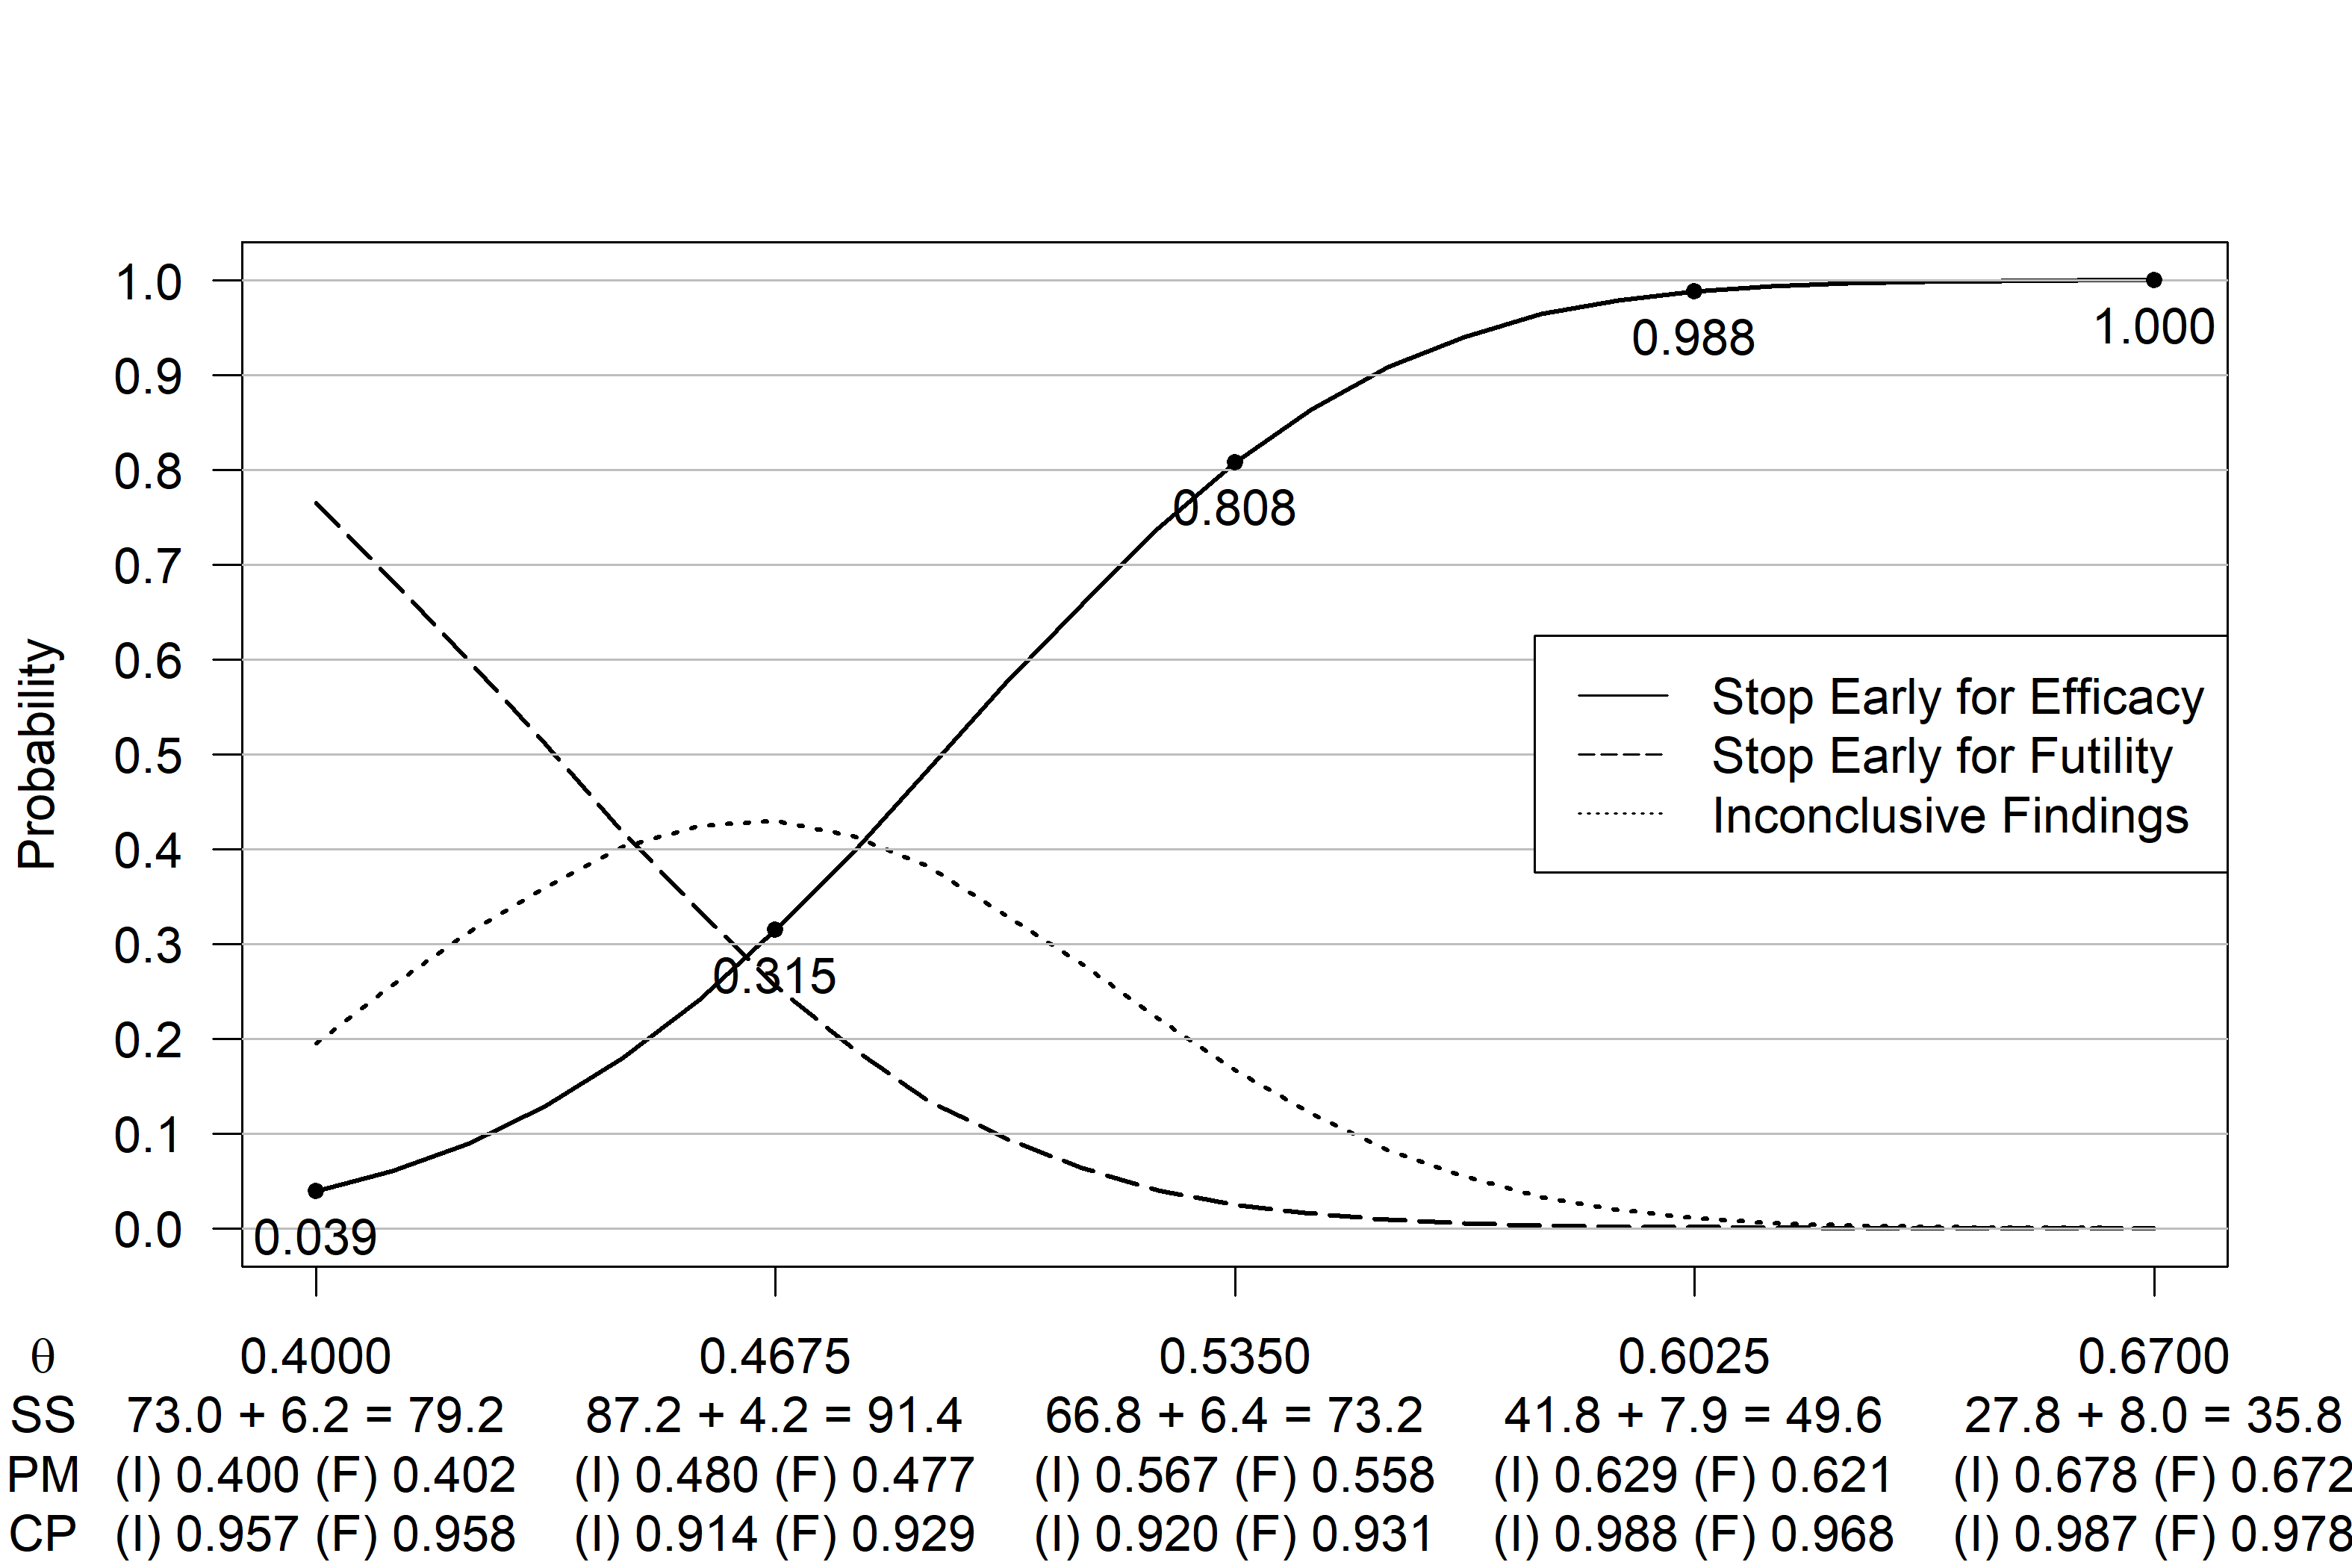
\includegraphics[width=6in]{P:/Bayesian-Sequential-Monitoring/00-paper/FIGURES/figure3a.png}
    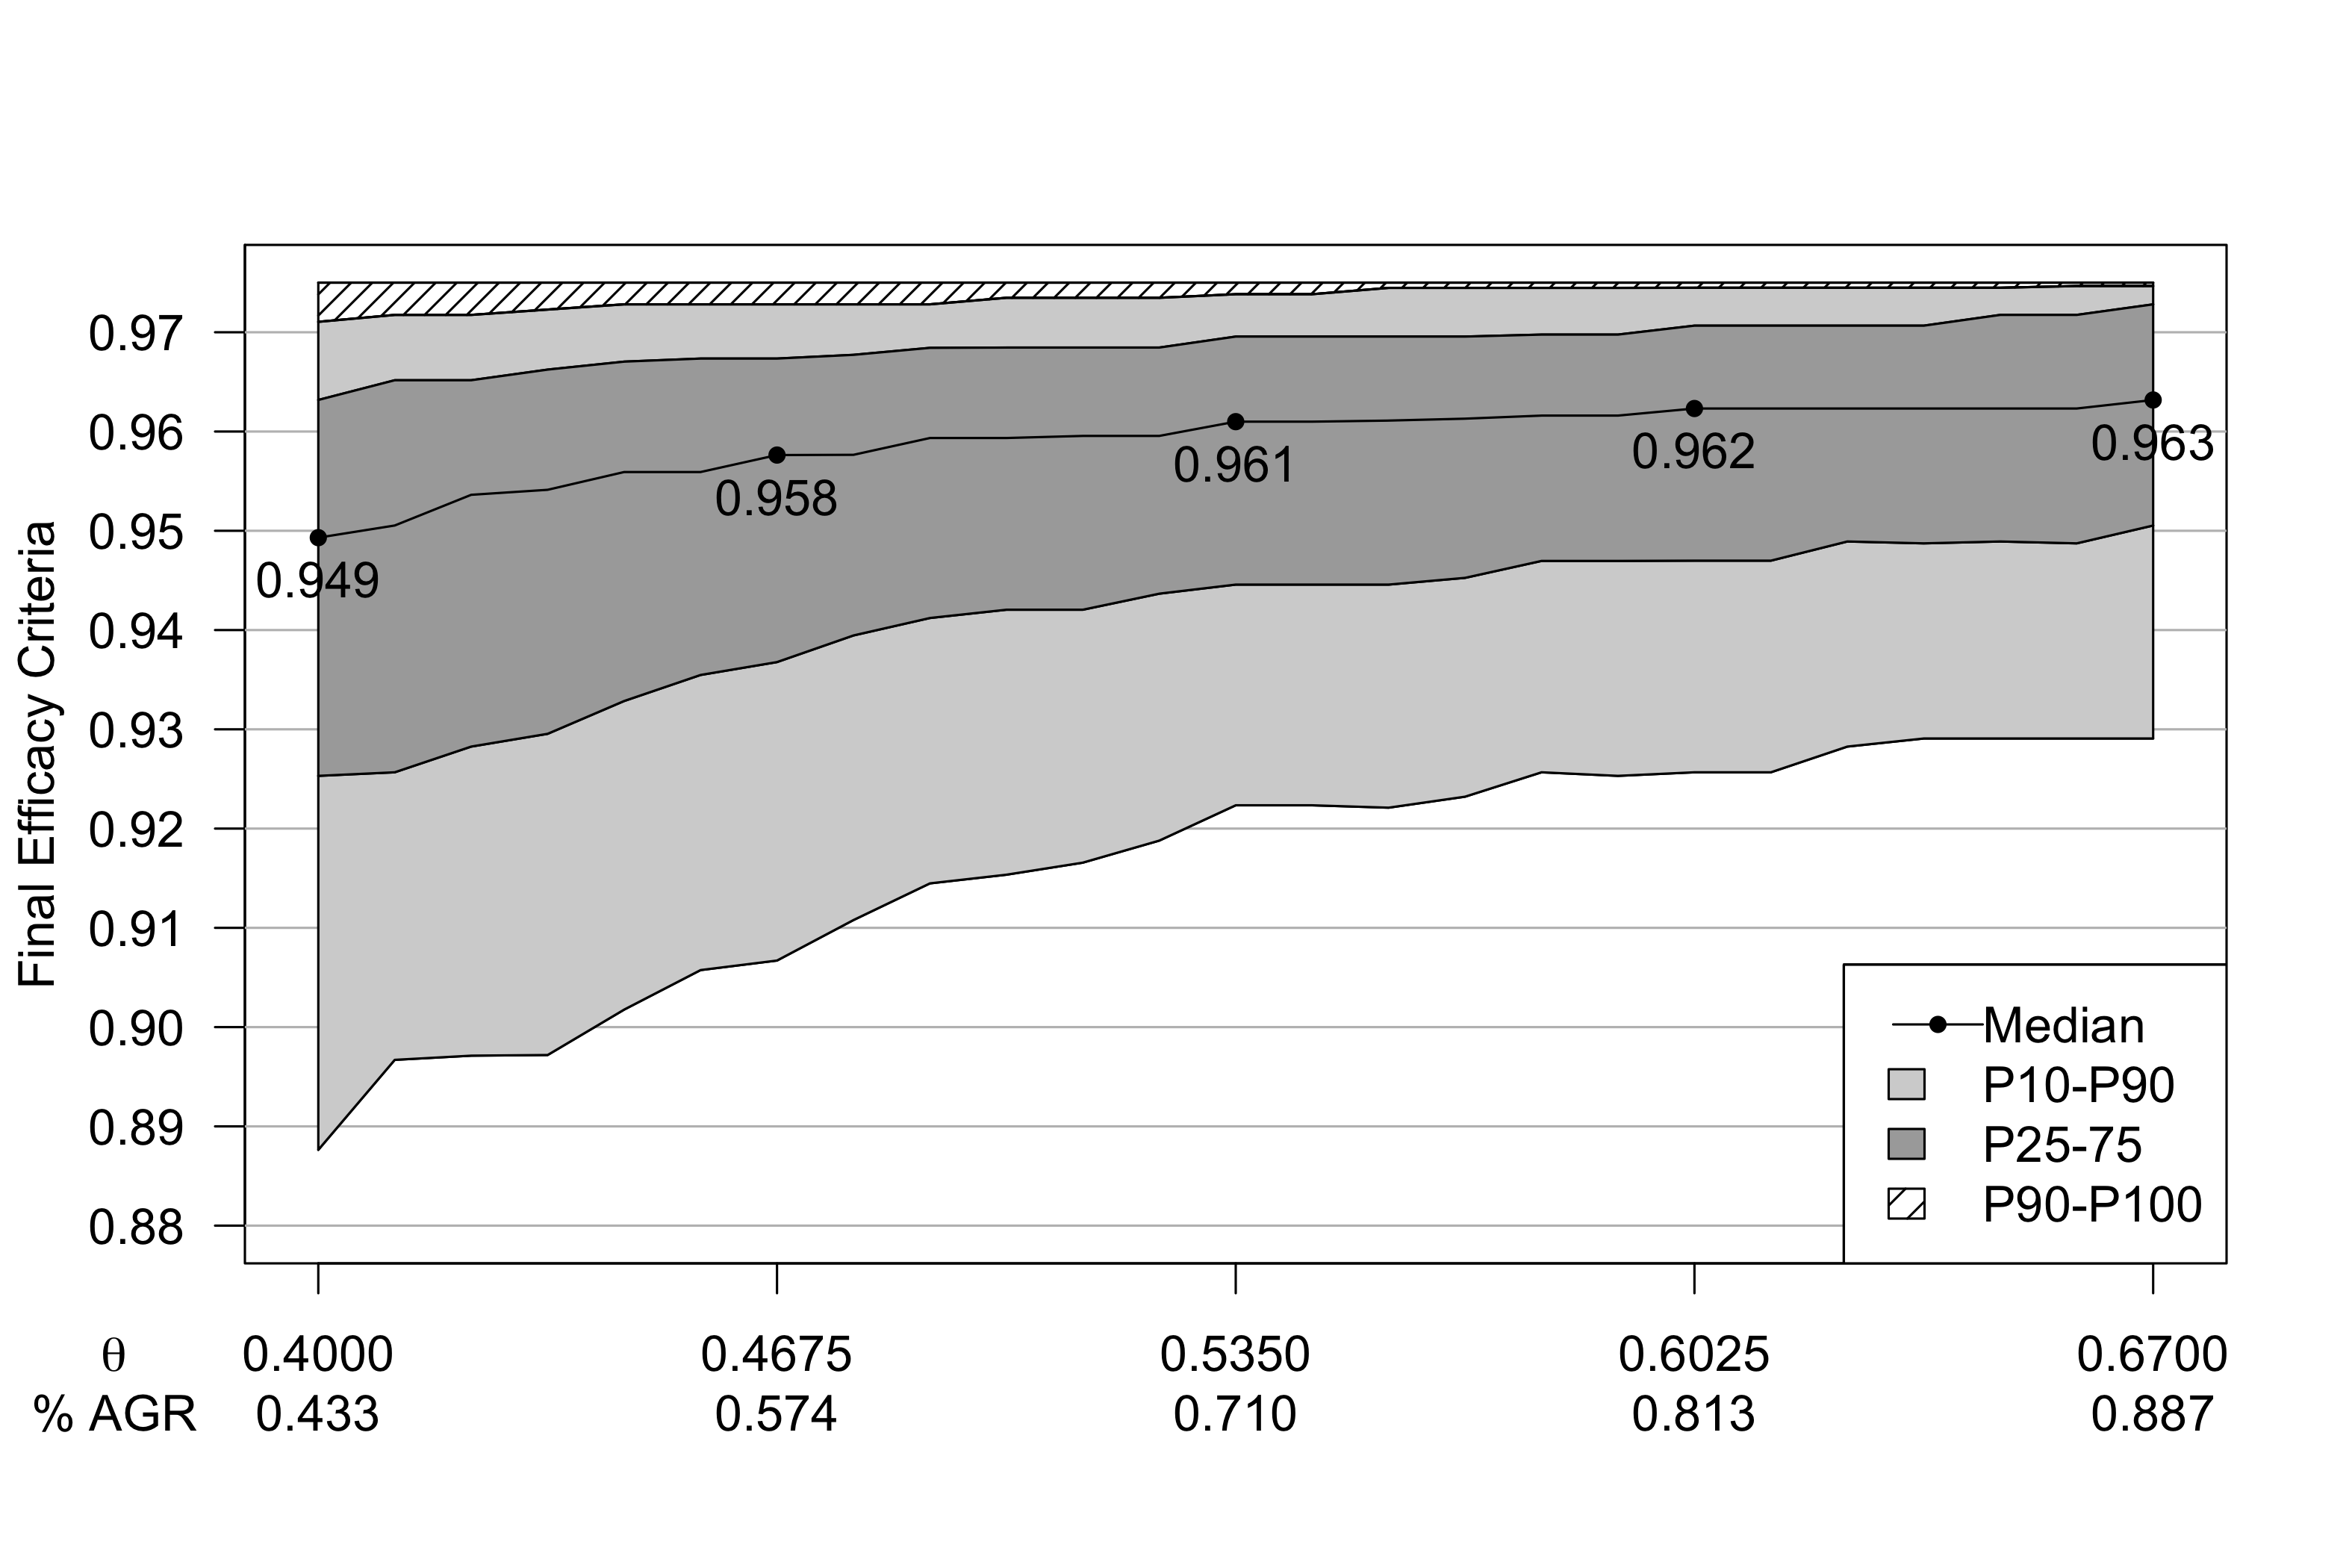
\includegraphics[width=6in]{P:/Bayesian-Sequential-Monitoring/00-paper/FIGURES/figure3b.png}
    \caption{A, Sequential design properties. (SS; sample size, PM; posterior mean, CP; coverage probability, (I); interim analysis, (F); final analysis) B, Distribution of final posterior probability given interim stoppage and evidence decrease ($\%$ AGR; Percent of agreement between final and interim posterior probabilities relative to $1-\epsilon$ threshold)}
	\label{fig:ex1.1}

\end{center}\end{figure}

%\subsubsection*{Vemurafenib Trial }
%``In this study, a response rate of 15\% at week
%8 was considered to be low, a response rate of
%45\% was considered to be high, and a response
%rate of 35\% was considered to be low but still
%desirable and indicative of efficacy. Assuming
%response rates as specified in the hypothesis testing, a power of 80\% for a high response rate and
%70\% for the low but still desirable response rate,
%and a two-sided alpha level of 0.1, we calculated
%that the number of patients required in each
%cohort would be 7, 13, or 19, depending on the
%results obtained."

\subsubsection{Type 1 error rate by the frequency of data monitoring}
Figure \ref{fig:ex1t1e} shows the probability of the efficacy criteria (\ref{eq:ex1efficacy}) being satisfied at an interim or final analysis when $\theta=\theta_0$. The monitoring frequency is 1 when an interim analysis is made after every completed outcome (i.e. fully sequential), and is 112 (the maximum sample size) if the only analysis is done at the maximum sample size. 

The probability of the efficacy criteria being (errantly) satisfied is the highest for a fully sequential design, and decreases as the monitoring frequency decreases. However, the probability of the efficacy criteria being satisfied with the final data is very low for any type of sequential monitoring (under 0.02 in all cases).
\begin{figure}\begin{center}

    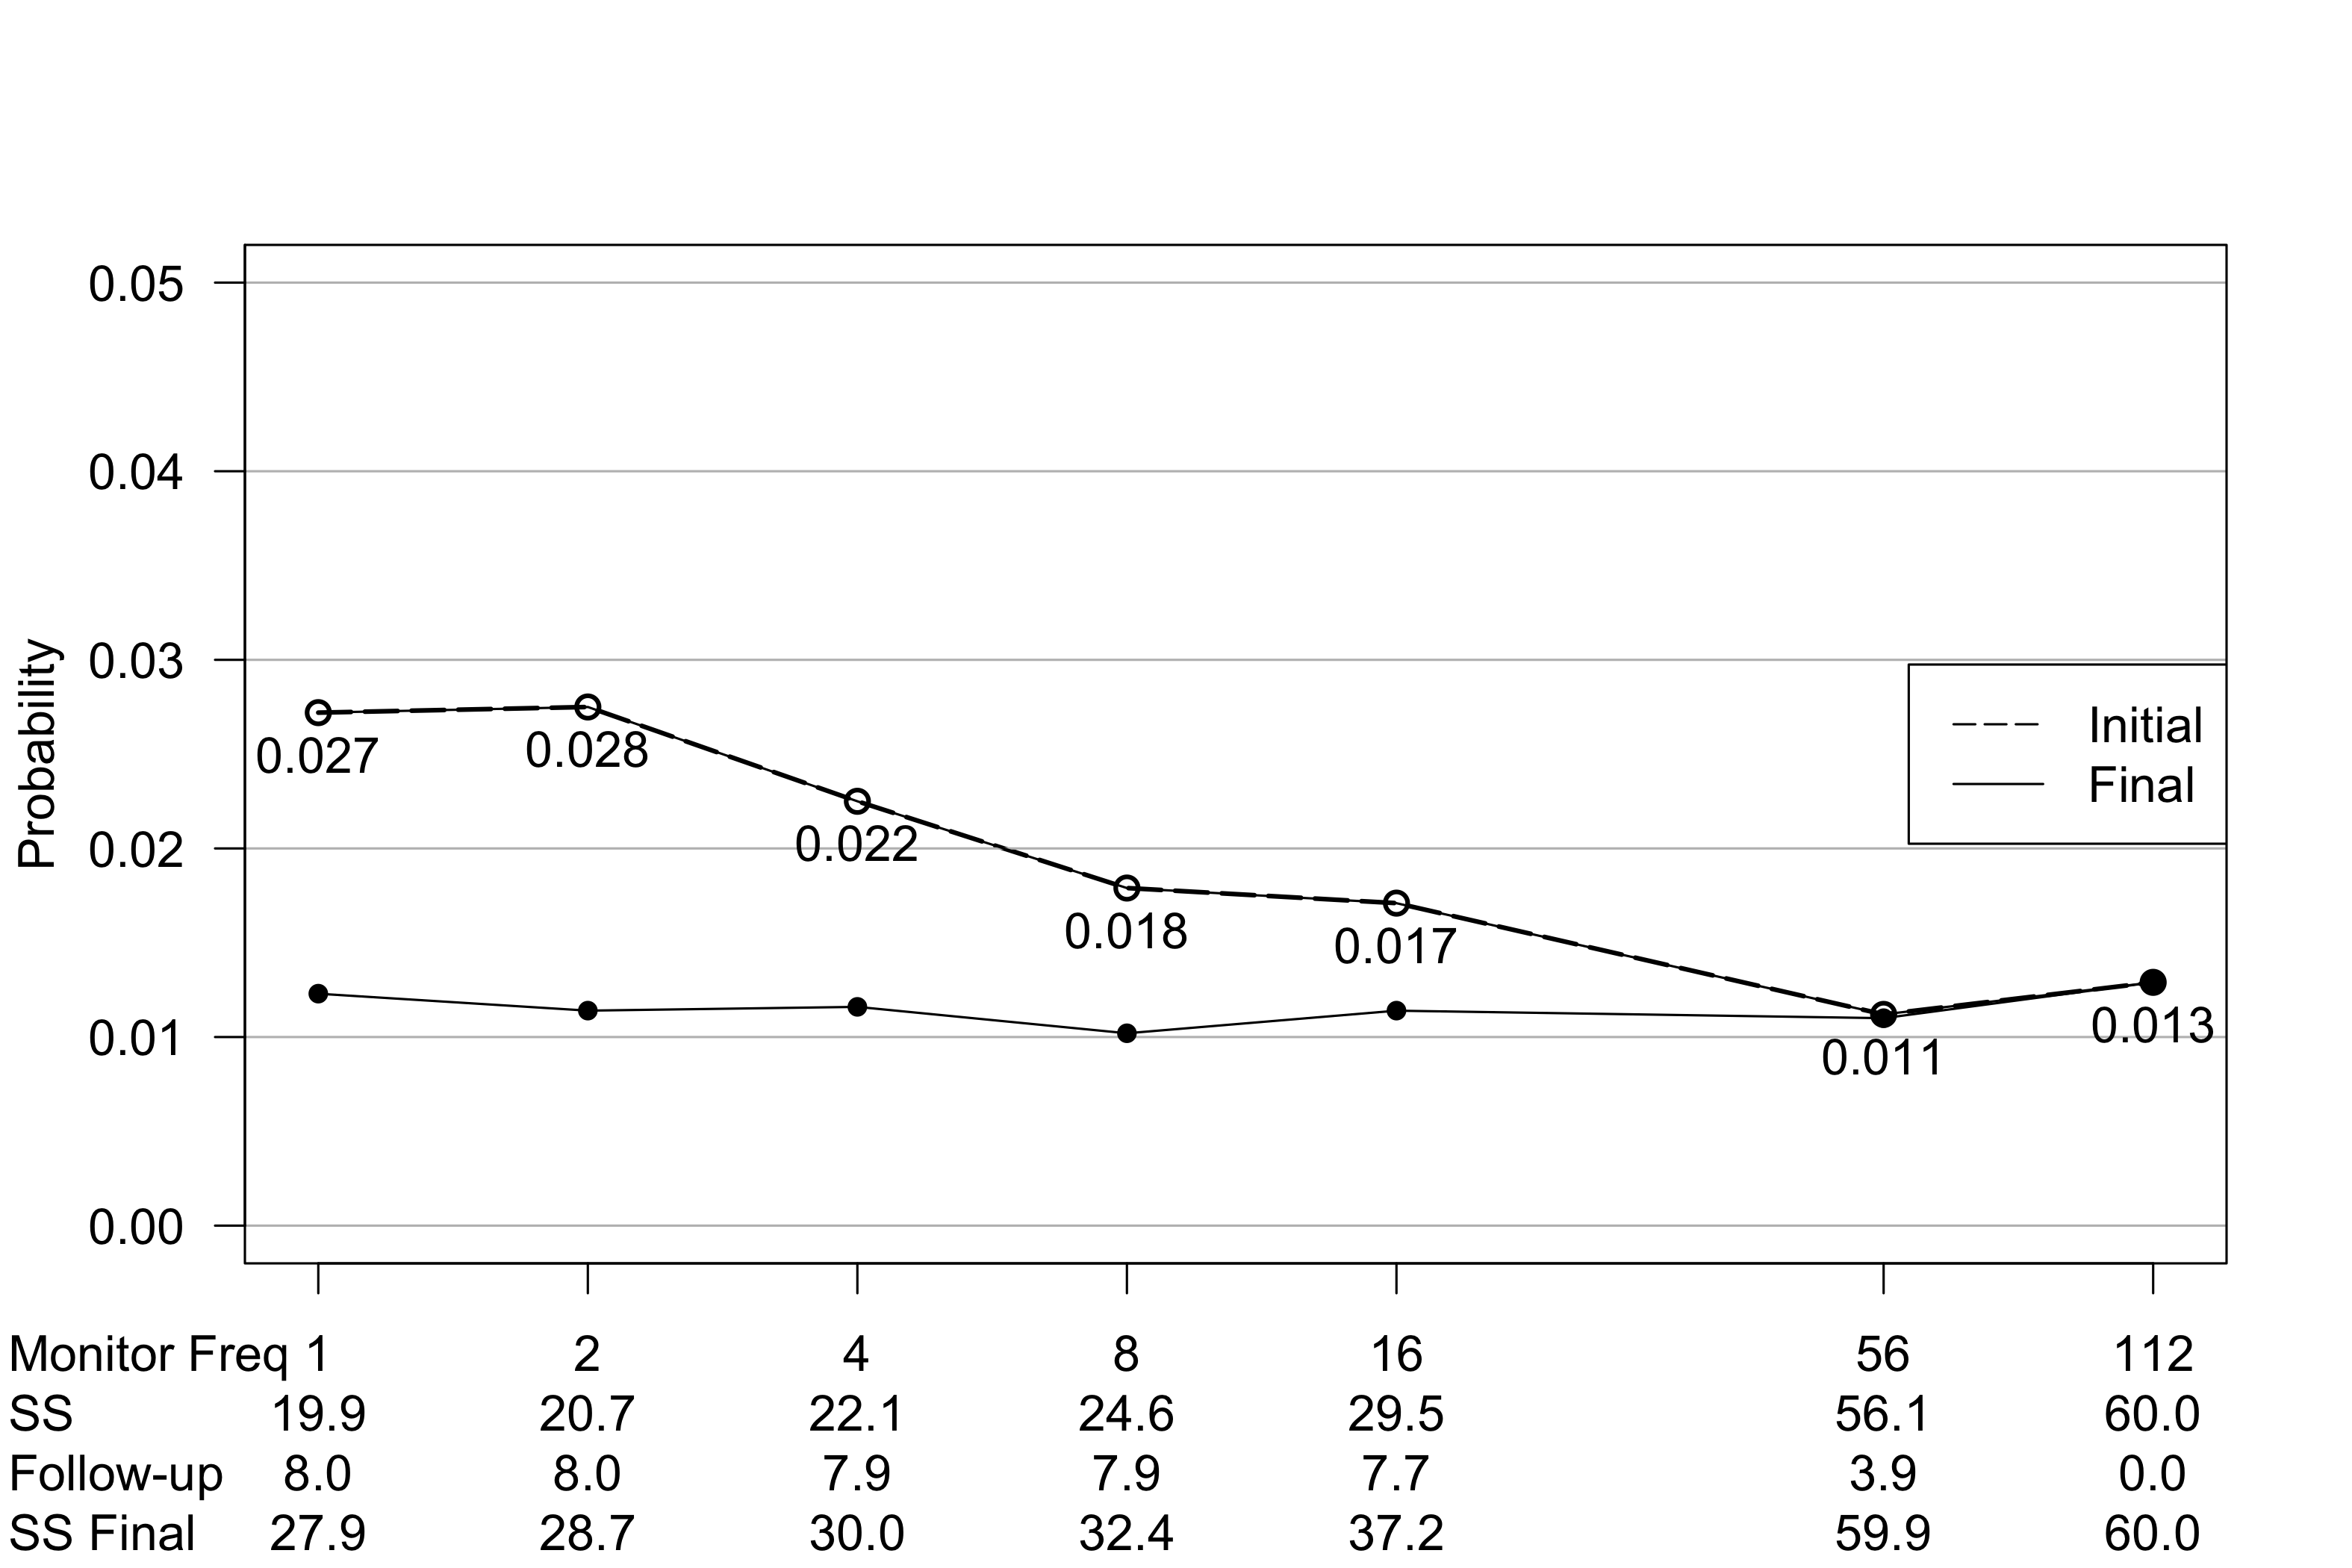
\includegraphics[width=6in]{P:/Bayesian-Sequential-Monitoring/00-paper/FIGURES/figure4.png}
    \caption{Probability of efficacy criteria being satisfied when $\theta=\theta_0$. SS; sample size. Monitor Freq; monitoring frequency.}
	\label{fig:ex1t1e}

%  \begin{subfigure}{7in}
%    \centering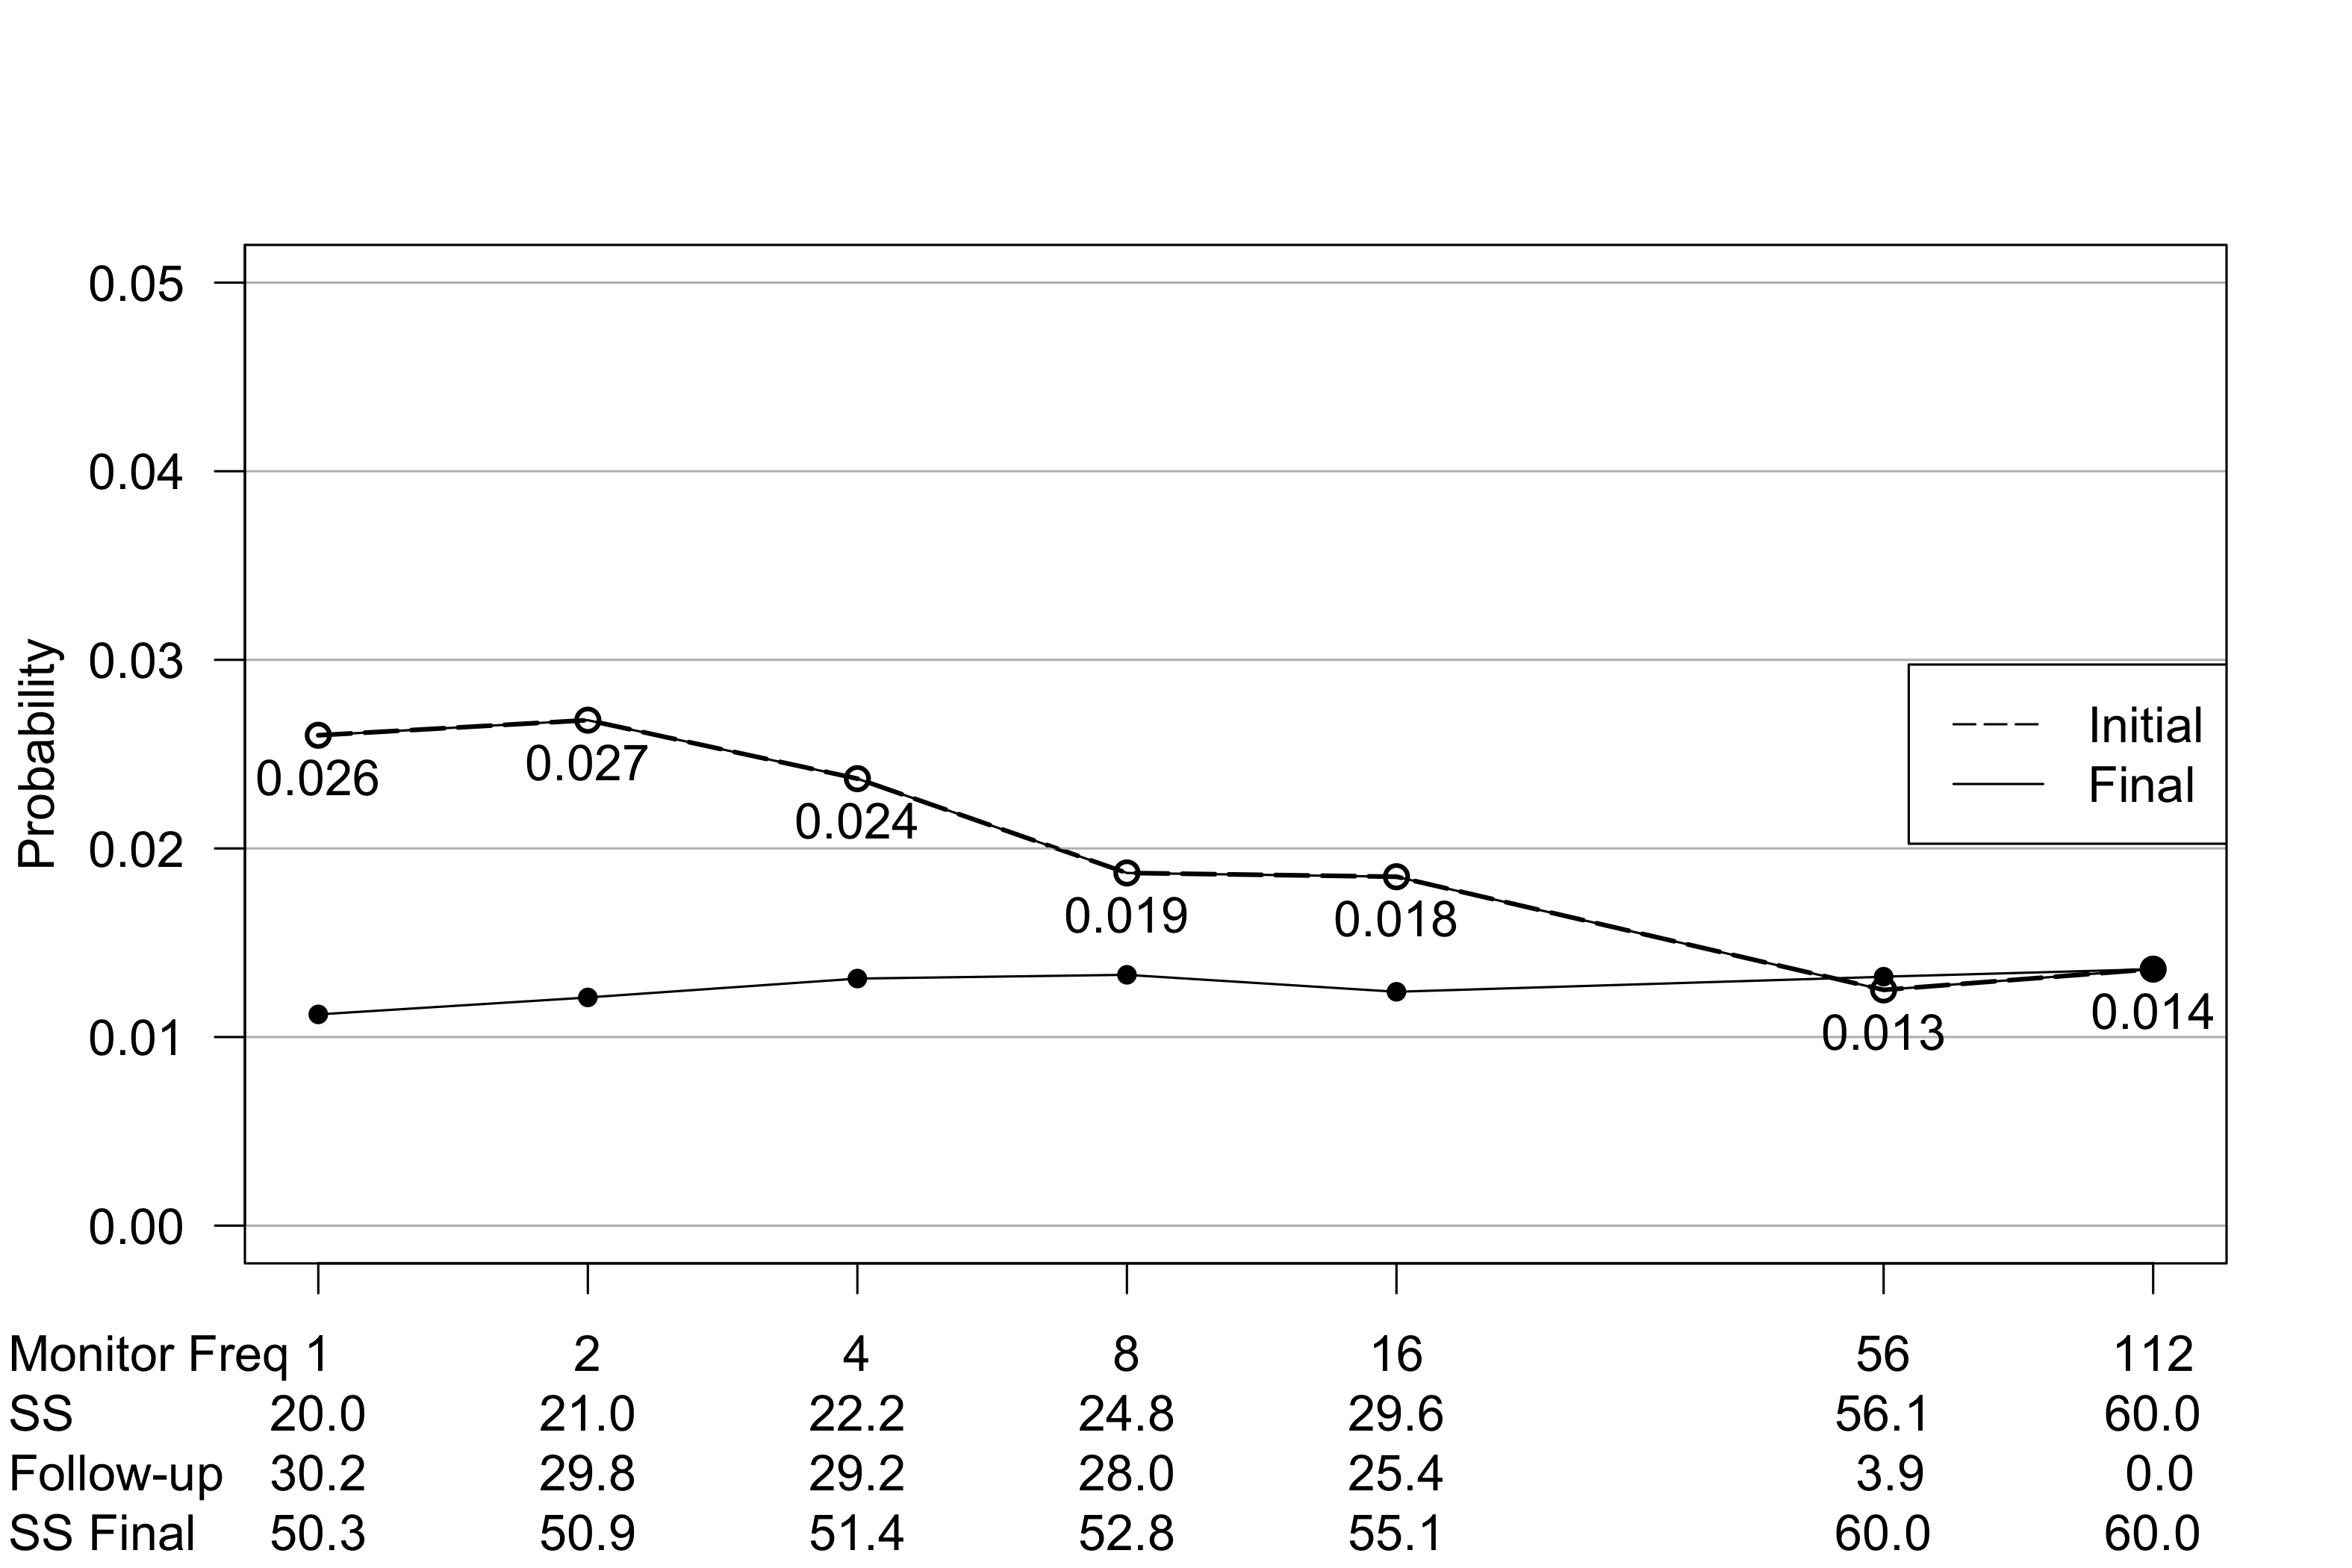
\includegraphics[width=7in]{P:/Bayesian-Sequential-Monitoring/00-paper/FIGURES/figureS1.png}
%    \caption{Caption text 2}
%  \end{subfigure}
 
\end{center}\end{figure}

%Even at the extreme case where an interim analysis is conducted after every outcome, the probability of stopping at the interim due to a promising result when the true response is at the null level is only $0.108$ (about double the nominal rate), and even in this situation the Type 1 error rate once follow-up is complete does not exceed $0.05$. Thus Bayesian sequential monitoring has good frequentist properties even with frequent interim analyses.
%\begin{itemize}
%\item The two sides of the discussion: first is what happens during the trial regarding sequential monitoring, such as \% of time stopping early vs. trial done to completion and expected sample size. Second is the final determination of efficacy or futility and how that relates to Type 1 Error and power. 
%\item  Remember the best case for sequential monitoring is slow enrollment relative to outcome ascertainment. Slow enrollment means there is a benefit to ending trial early and reach a conclusion faster. Outcome ascertainment needs to be somewhat fast to ensure a good \# of outcomes are generated.
%\end{itemize}
%\begin{itemize}
%\item Want to highlight that the ultimate inference will have no Type 1 error inflation. At this point the ultimate inference for efficacy is still made with skeptical prior.
%\item Label lines nicely.
%\item ``Only bad thing to do is to stop learning"
%\item Enrollment rate and \% of ongoing data as operating characteristics are interesting ideas, but focus on the plots already created.
%\item Mat: Scaling on \# of subjects in each interim analysis rather than \# of interim analyses (e.g. flip X axis). Make labels go vertical or diagonal.
%\end{itemize}

\subsection{Parallel Two-Group Design with Binary Endpoint}\label{sec:example2}
\subsubsection{Motivating example}
Consider the trial ``The Pediatric Lupus Trial of Belimumab Plus Background Standard Therapy (PLUTO)" (NCT01649765). Subjects were randomized to Belimumab 10mg/kg or placebo, and the primary endpoint was response at week 52. Response was measured by improvement in disease severity scores. The goal was to test for superiority of Belimumab to placebo. 

The study start date was September 7, 2012, and the primary completion date was January 24, 2018. Since the follow-up period is 52 weeks the last enrollment is estimated to be a year prior to the primary competition date yielding an average enrollment rate of one enrollment per $17.2$ days.

The study design included enrollment of 100 subjects, the first 24 subjects randomized in a 5:1 ratio (Belimumab:placebo) and the remaining 76 subjects would be randomized in a 1:1 allocation ratio. Therefore, 58 subjects would be randomized to Belimumab and 42 to placebo. The sample size was based on feasibility constraints rather than a power calculation, and the study was terminated after 93 subjects enrolled.

\subsubsection{Model formulation \& prior elicitation}
The data $\mathbf{D}$ are assumed to be independent Bernoulli random variables with response probability $\theta_0$ for the placebo group and $\theta_1$ for the treatment (IP for investigational product) group. The null response value for the difference $\delta=\theta_1-\theta_0=0$ is  and a highly efficacious response probability is $\delta=\theta_1-\theta_0=0.12$. Consider the hypothesis testing of IP superiority to control $H_0:\theta_1-\theta_0\leq 0\text{ vs. }H_1: \theta_1-\theta_0>0$. An estimate for the treatment probability from adult trials is $\theta_1=0.51$.

The priors will be chosen based on the generalized normal distribution (\ref{eq:generalizednormalkernel}) based on the joint specification in (\ref{eq:generalized_normal_joint}) and truncated to the unit square 

The skeptical and enthusiastic priors will have the same component for
\begin{align}
\pi(\theta_0)\propto \exp\left\{-\left(\frac{|\theta_0-\mu|}{\alpha}\right)^{\beta}\right\}\times I(\theta_0 \in [0,1])
\end{align}
The location parameter is chosen to be $\mu=\theta_1-\delta_E=0.39$. The shape and scale parameters $\alpha$ and $\beta$ are chosen so that the prior is flat in the region $\mu\pm 0.10$ and is shown in Figure \ref{fig:figure5}(E). 

The skeptical and enthusiastic priors are differentiated by their parameterizations for 
\begin{align}
\pi_S(\theta_1|\theta_0)\propto&\exp\left\{-\left(\frac{|\theta_1-\theta_0-\delta_0|}{\alpha_S}\right)^{\beta_S}\right\}\times f_S(\theta_0) \times I((\theta_0,\theta_1)\in [0,1]\times[0,1])\\
\pi_E(\theta_1|\theta_0)\propto&\exp\left\{-\left(\frac{|\theta_1-\theta_0-\delta_1|}{\alpha_E}\right)^{\beta_E}\right\}\times f_E(\theta_0) \times I((\theta_0,\theta_1)\in [0,1]\times[0,1])
\end{align}

The values $\beta_S$ and $\beta_E$ are pre-specified and $\alpha_S$ and $\alpha_E$ are chosen to satisfy the tail-probability conditions 
(\ref{eq:ex2enthcondition})-(\ref{eq:ex2skptcondition}).

The complete skeptical and enthusiastic priors are then given by 
\begin{align}
\pi_S(\theta_0,\theta_1)\propto&\exp\left\{-\left(\frac{|\theta_0-\mu|}{\alpha}\right)^{\beta}\right\}\times \exp\left\{-\left(\frac{|\theta_1-\theta_0-\delta_0|}{\alpha_S}\right)^{\beta_S}\right\}\times I((\theta_0,\theta_1)\in [0,1]\times[0,1])\label{eq:ex2skpt}\\
\pi_E(\theta_0,\theta_1)\propto&\exp\left\{-\left(\frac{|\theta_0-\mu|}{\alpha}\right)^{\beta}\right\}\times \exp\left\{-\left(\frac{|\theta_1-\theta_0-\delta_1|}{\alpha_E}\right)^{\beta_E}\right\}\times I((\theta_0,\theta_1)\in [0,1]\times[0,1])\label{eq:ex2enth}.
\end{align}

The joint priors $\pi_S(\theta_0,\theta_1)$ $\pi_E(\theta_0,\theta_1)$ as well as the marginal priors $\pi_S(\theta_1-\theta_0)$, $\pi_E(\theta_1-\theta_0)$ are shown in Figure \ref{fig:figure5}.
%
%where $c_S$ and $c_E$ are normalizing constants. The values of $\alpha_S$ and $\alpha_{S1}$ are chosen such that $P(\theta_1-\theta_0>0.1|\pi_S)=0.05$. Similarly, $\alpha_E$ and $\alpha_{E1}$ are chosen such that $P(\theta_1-\theta_0\leq0|\pi_E)=0.05$.

%\begin{align*}
%\pi(\theta_0,\theta_1)\propto& \hspace{0.05in}exp \left\{-\frac{1}{2}\left|\frac{(\theta_1-\theta_0)-\delta}{\alpha}\right|^\alpha\right\}
%\end{align*}


%Here we wish to elicit pessimistic and enthusiastic priors consistent with the following:
% \begin{enumerate}
%  \item The control group response probability is expected to be approximately $0.20$ and investigators are relatively sure
%		    that the it will be between 0.5 and 0.35.
%				
%	\item The IP group response probability is likely to provide an improvement of approximately 0.20.
%\end{enumerate}

Enrollment will proceed until one of the following three conditions are satisfied:
\begin{align}
\text{Efficacy criteria (EFF): }&P(\theta_1-\theta_0>\delta_0|\mathbf{D},\pi_S)\geq 1-\epsilon \label{eq:ex2efficacy}\\
\text{Futility criteria (FUT): }&P\left(\theta_1-\theta_0 \leq \frac{\delta_0+\delta_1}{2}\Big|\mathbf{D},\pi_E\right)\geq 1-\epsilon
\label{eq:ex2futility}\\
\text{Maximum sample size: }&N=100 \text{ patient outcomes}\label{eq:ex2maxss}
\end{align}

An interim analysis is competed after every 2 subjects have completed outcomes.

\subsubsection{Preposterior Analysis of Operating Characteristics}\label{sec:ex2operatingcharacteristics}
A mixture prior $\pi_I$ of the form (\ref{eq:inference_prior}) is used for efficency monitoring where the choice of $\omega$ is chosen at the outset to be in the set $\{0.25,0.5,0.75,1\}$. Note that $\omega=1$ corresponds to the traditional skeptical prior and $\omega=0.5$ gives equal weight to the skeptical and enthusiastic components. When $\omega=0.25$ most of the weight to the enthusiastic component.

Figure \ref{fig:ex2varyomega} shows the probability of stopping early for efficacy (satisfying (\ref{eq:ex2efficacy})) based on the choice of $\omega$ used in the mixture prior for efficiency monitoring, and the associated sample sizes. Note that only in the case of $\omega=0.25$ is the probability of stopping the trial early for efficacy near 50\% when $\delta=\delta_1$. Also, only in the case of $\omega=0.25$ is the expected sample size less than 90. Therefore, for this design, the monitoring prior for efficacy has to be mostly enthusiastic in order for reasonable efficacy conditions.

\begin{figure}\begin{center}
    \centering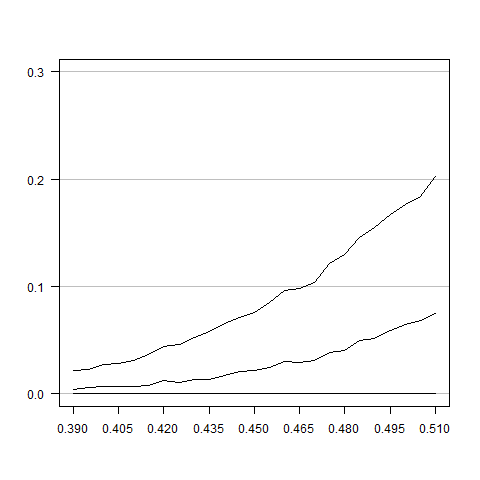
\includegraphics[width=7in]{P:/Bayesian-Sequential-Monitoring/00-paper/FIGURES/figure6.png}
    \caption{Probability of stopping for efficacy and associated sample sizes by choice of $\omega$ used in a mixture inference prior for efficacy monitoring.}
\label{fig:varyomega}
 \end{center}\end{figure}


\section{Discussion}



\section{Supplementary material}


\subsection{Type 1 error rate depending on enrollment schemes}
Recall Figure \ref{fig:ex1t1e} from Section \ref{sec:example1} which showed Type 1 error properties for the single-arm design. Figure \ref{fig:ex1t1e_longer} shows results from a design that has a longer follow-up period. The interim sample sizes are the same for each monitoring frequency, however, the final sample sizes under the longer follow-up designs are much larger (over 20 subjects in follow-up for monitoring frequencies of 8 or fewer, compared to approximately 6 subjects in the shorter follow-up designs). The final probability of efficacy criteria being satisfied is generally slightly lower in the longer follow-up design, which is what we would expect since the larger final sample size contains more data consistent with a null result.
\begin{figure}\begin{center}

   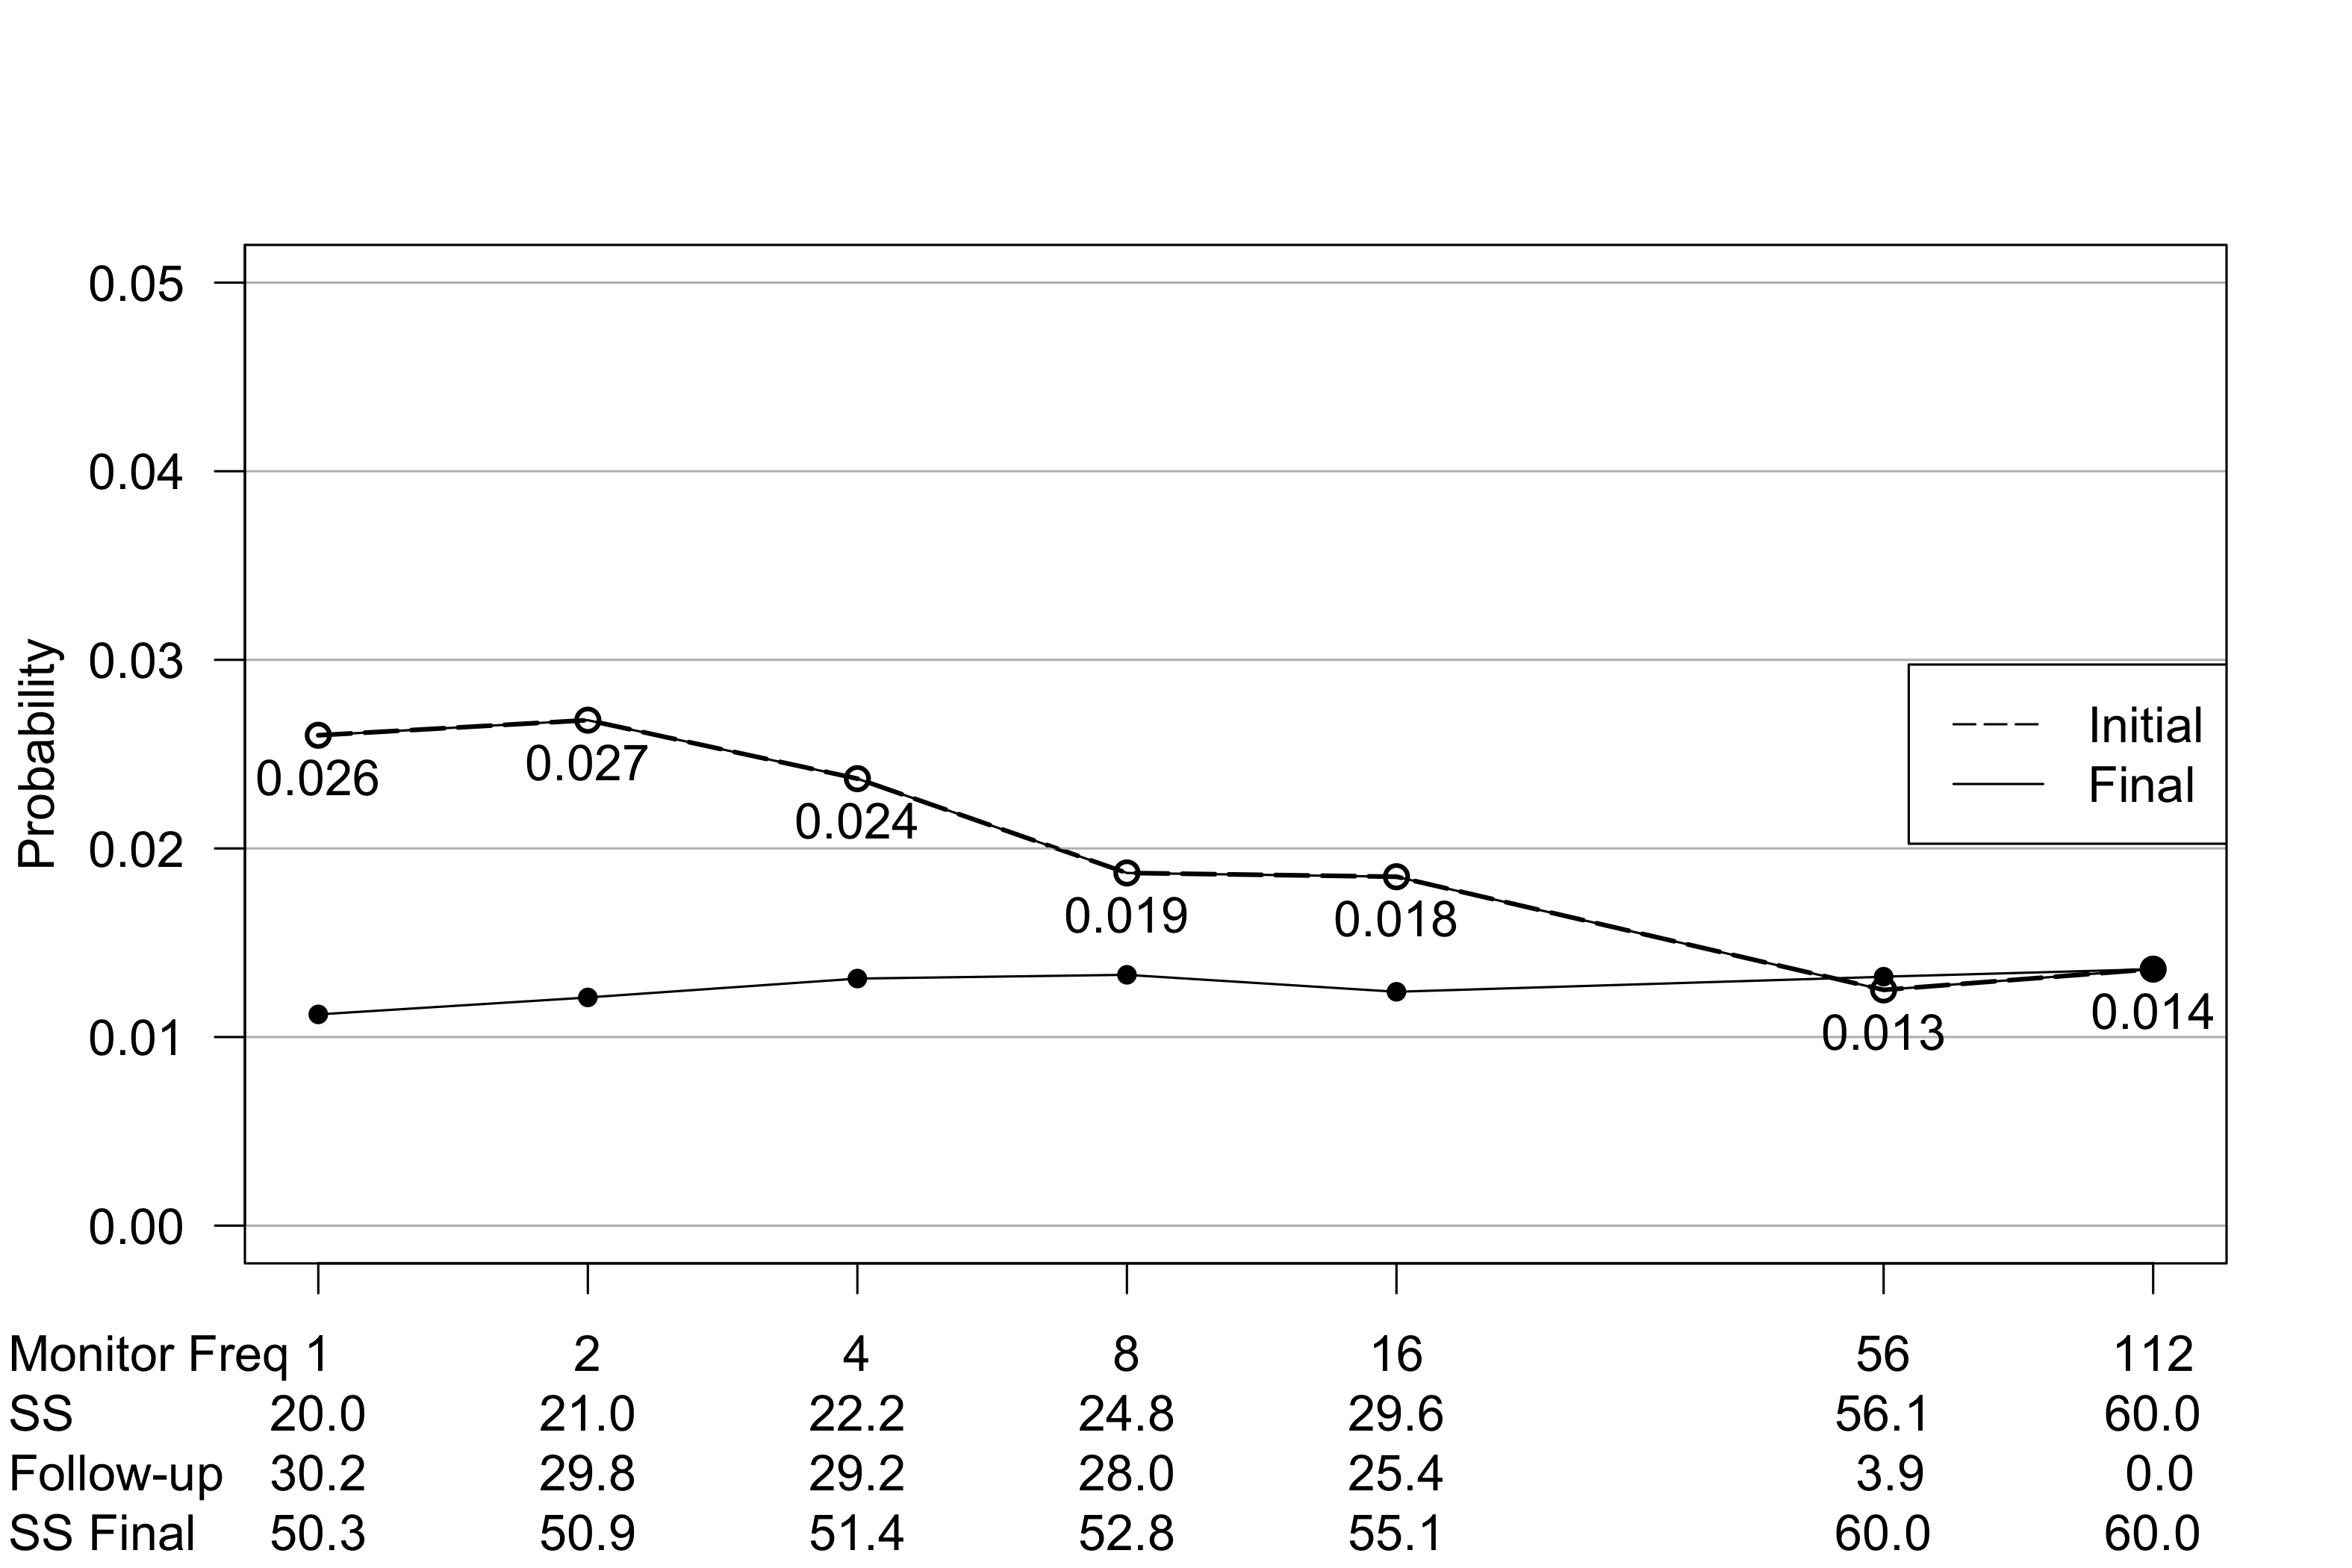
\includegraphics[width=6in]{P:/Bayesian-Sequential-Monitoring/00-paper/FIGURES/figureS1.png}
    \caption{Single arm design from Example \ref{sec:example1} with a longer follow-up period. Probability of efficacy criteria being satisfied when $\theta=\theta_0$. SS; sample size. Monitor Freq; monitoring frequency.}
	\label{fig:ex1t1e_longer}

\end{center}\end{figure}


\subsection{Robustness of parameterizations of monitoring priors}\label{sec:priorRobustness}
The analyses done in Section \ref{sec:example1} used a concentrate skeptical prior and default enthusiastic prior. In this section we show the four possible designs using the combinations of skeptical and enthusiastic prior given in Figure \ref{fig:figure1}.

Figures \ref{fig:robustness1}-\ref{fig:robustness2} shows what happens when the enthusiastic prior shifts from default to flattened, with the skeptical prior remaining fixed. Note that in the region between $\theta_0$ and $\frac{\theta_0+\theta_1}{2}$ as the enthusiastic prior shifts from default to flattened, (a) the probability of stopping early for futility increases (b) the probability of inconclusive findings decreases and (c) the intermediate and final sample sizes decrease. This is because the enthusiastic prior gives more mass in for this region of $\theta$. The flattened enthusiastic prior was used in Section \ref{sec:example1} to enhance the ability of futility monitoring to reduce the sample size.

Contrasting \ref{fig:robustness1} and \ref{fig:robustness2}, we see that the probability of stopping early for efficacy is much higher at $\theta_0$ when the default skeptical prior is used rather than the concentrated skeptical prior. This is because the default skeptical prior has less mass around $\theta=\theta_0$, therefore it is easier to convince the skeptic that $\theta>\theta_0$ under the null result $\theta=\theta_0$. The concentrated skeptical prior was used in Section \ref{sec:example1} to limit this probability and provide better Type 1 error control.

The choice of skeptical and enthusiastic prior affects the analysis, and their specification (e.g. default, skeptical, enthusiastic) should be made with these properties in mind.

\begin{figure}\begin{center}

 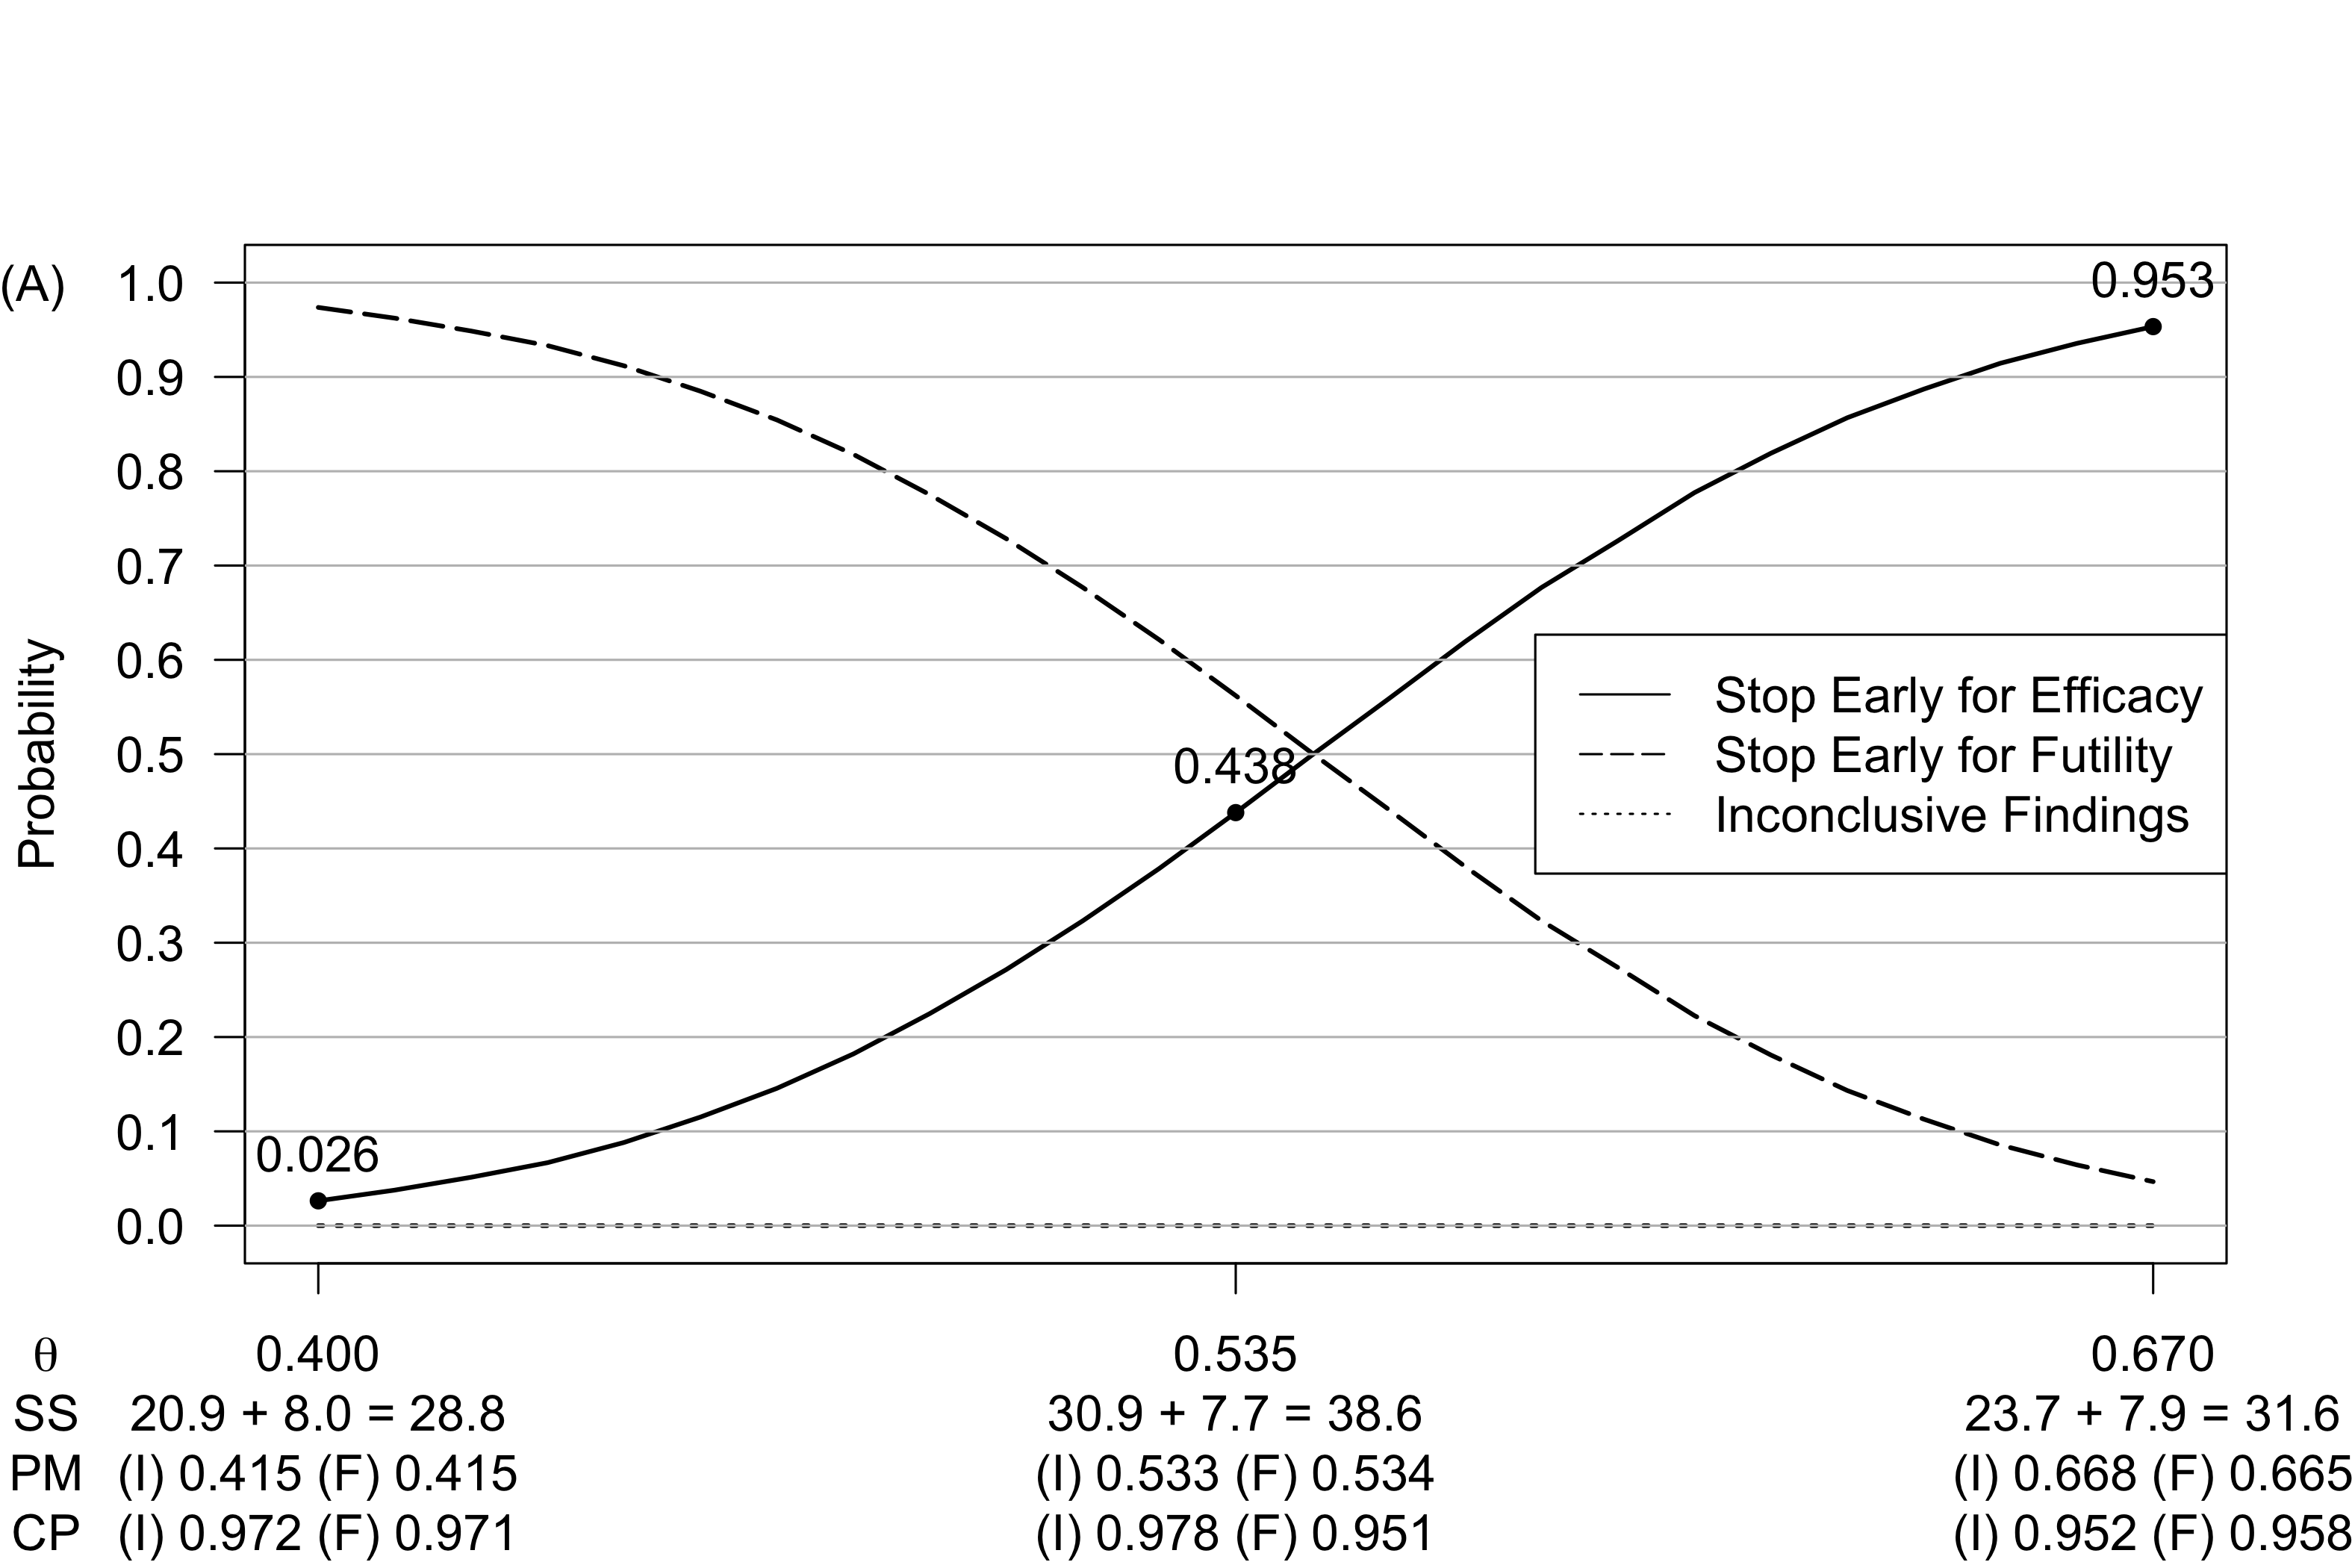
\includegraphics[width=7in]{P:/Bayesian-Sequential-Monitoring/00-paper/FIGURES/figureS2a.png}
 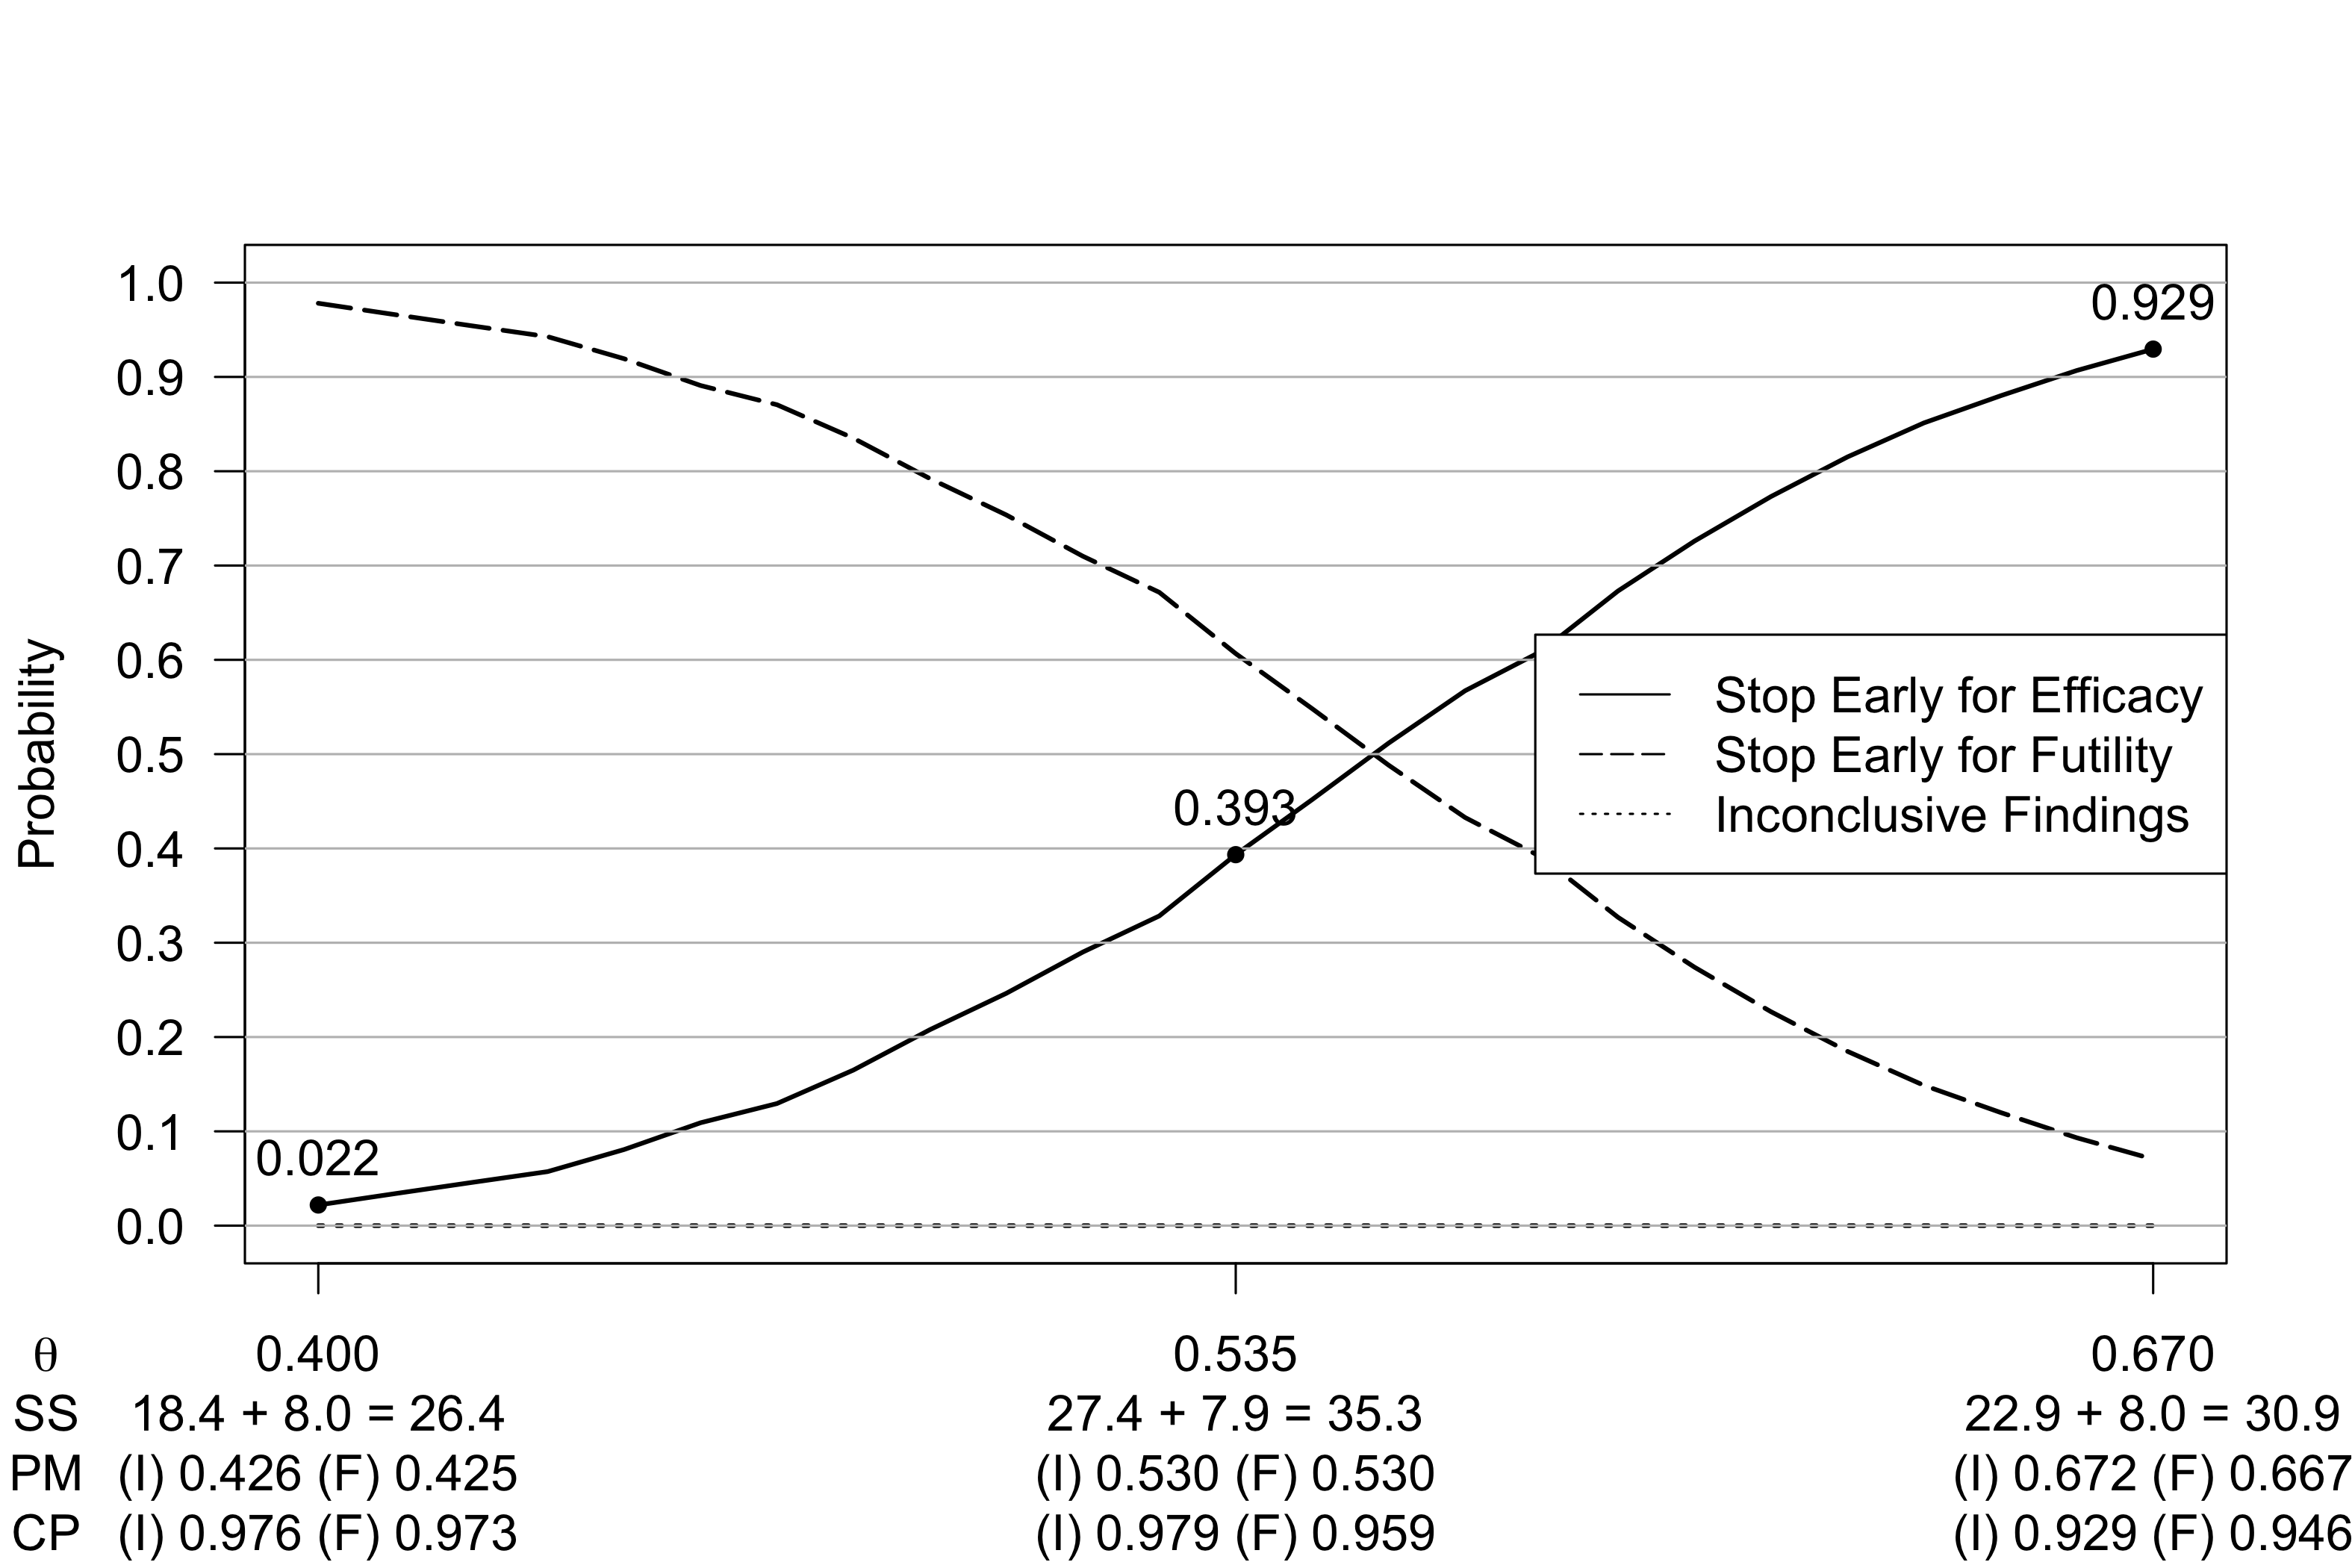
\includegraphics[width=7in]{P:/Bayesian-Sequential-Monitoring/00-paper/FIGURES/figureS2b.png}
 \caption{Modification of enthusiastic prior parameterization in Example \ref{sec:example1}. A, default enthusiastic prior (Figure \ref{fig:figure1}(c)). B, flattened enthusiastic prior (Figure \ref{fig:figure1}(d)). Both designs use concentrated skeptical prior (Figure \ref{fig:figure1}(b)).}
\label{fig:robustness1}
\end{center}\end{figure}

\begin{figure}\begin{center}

 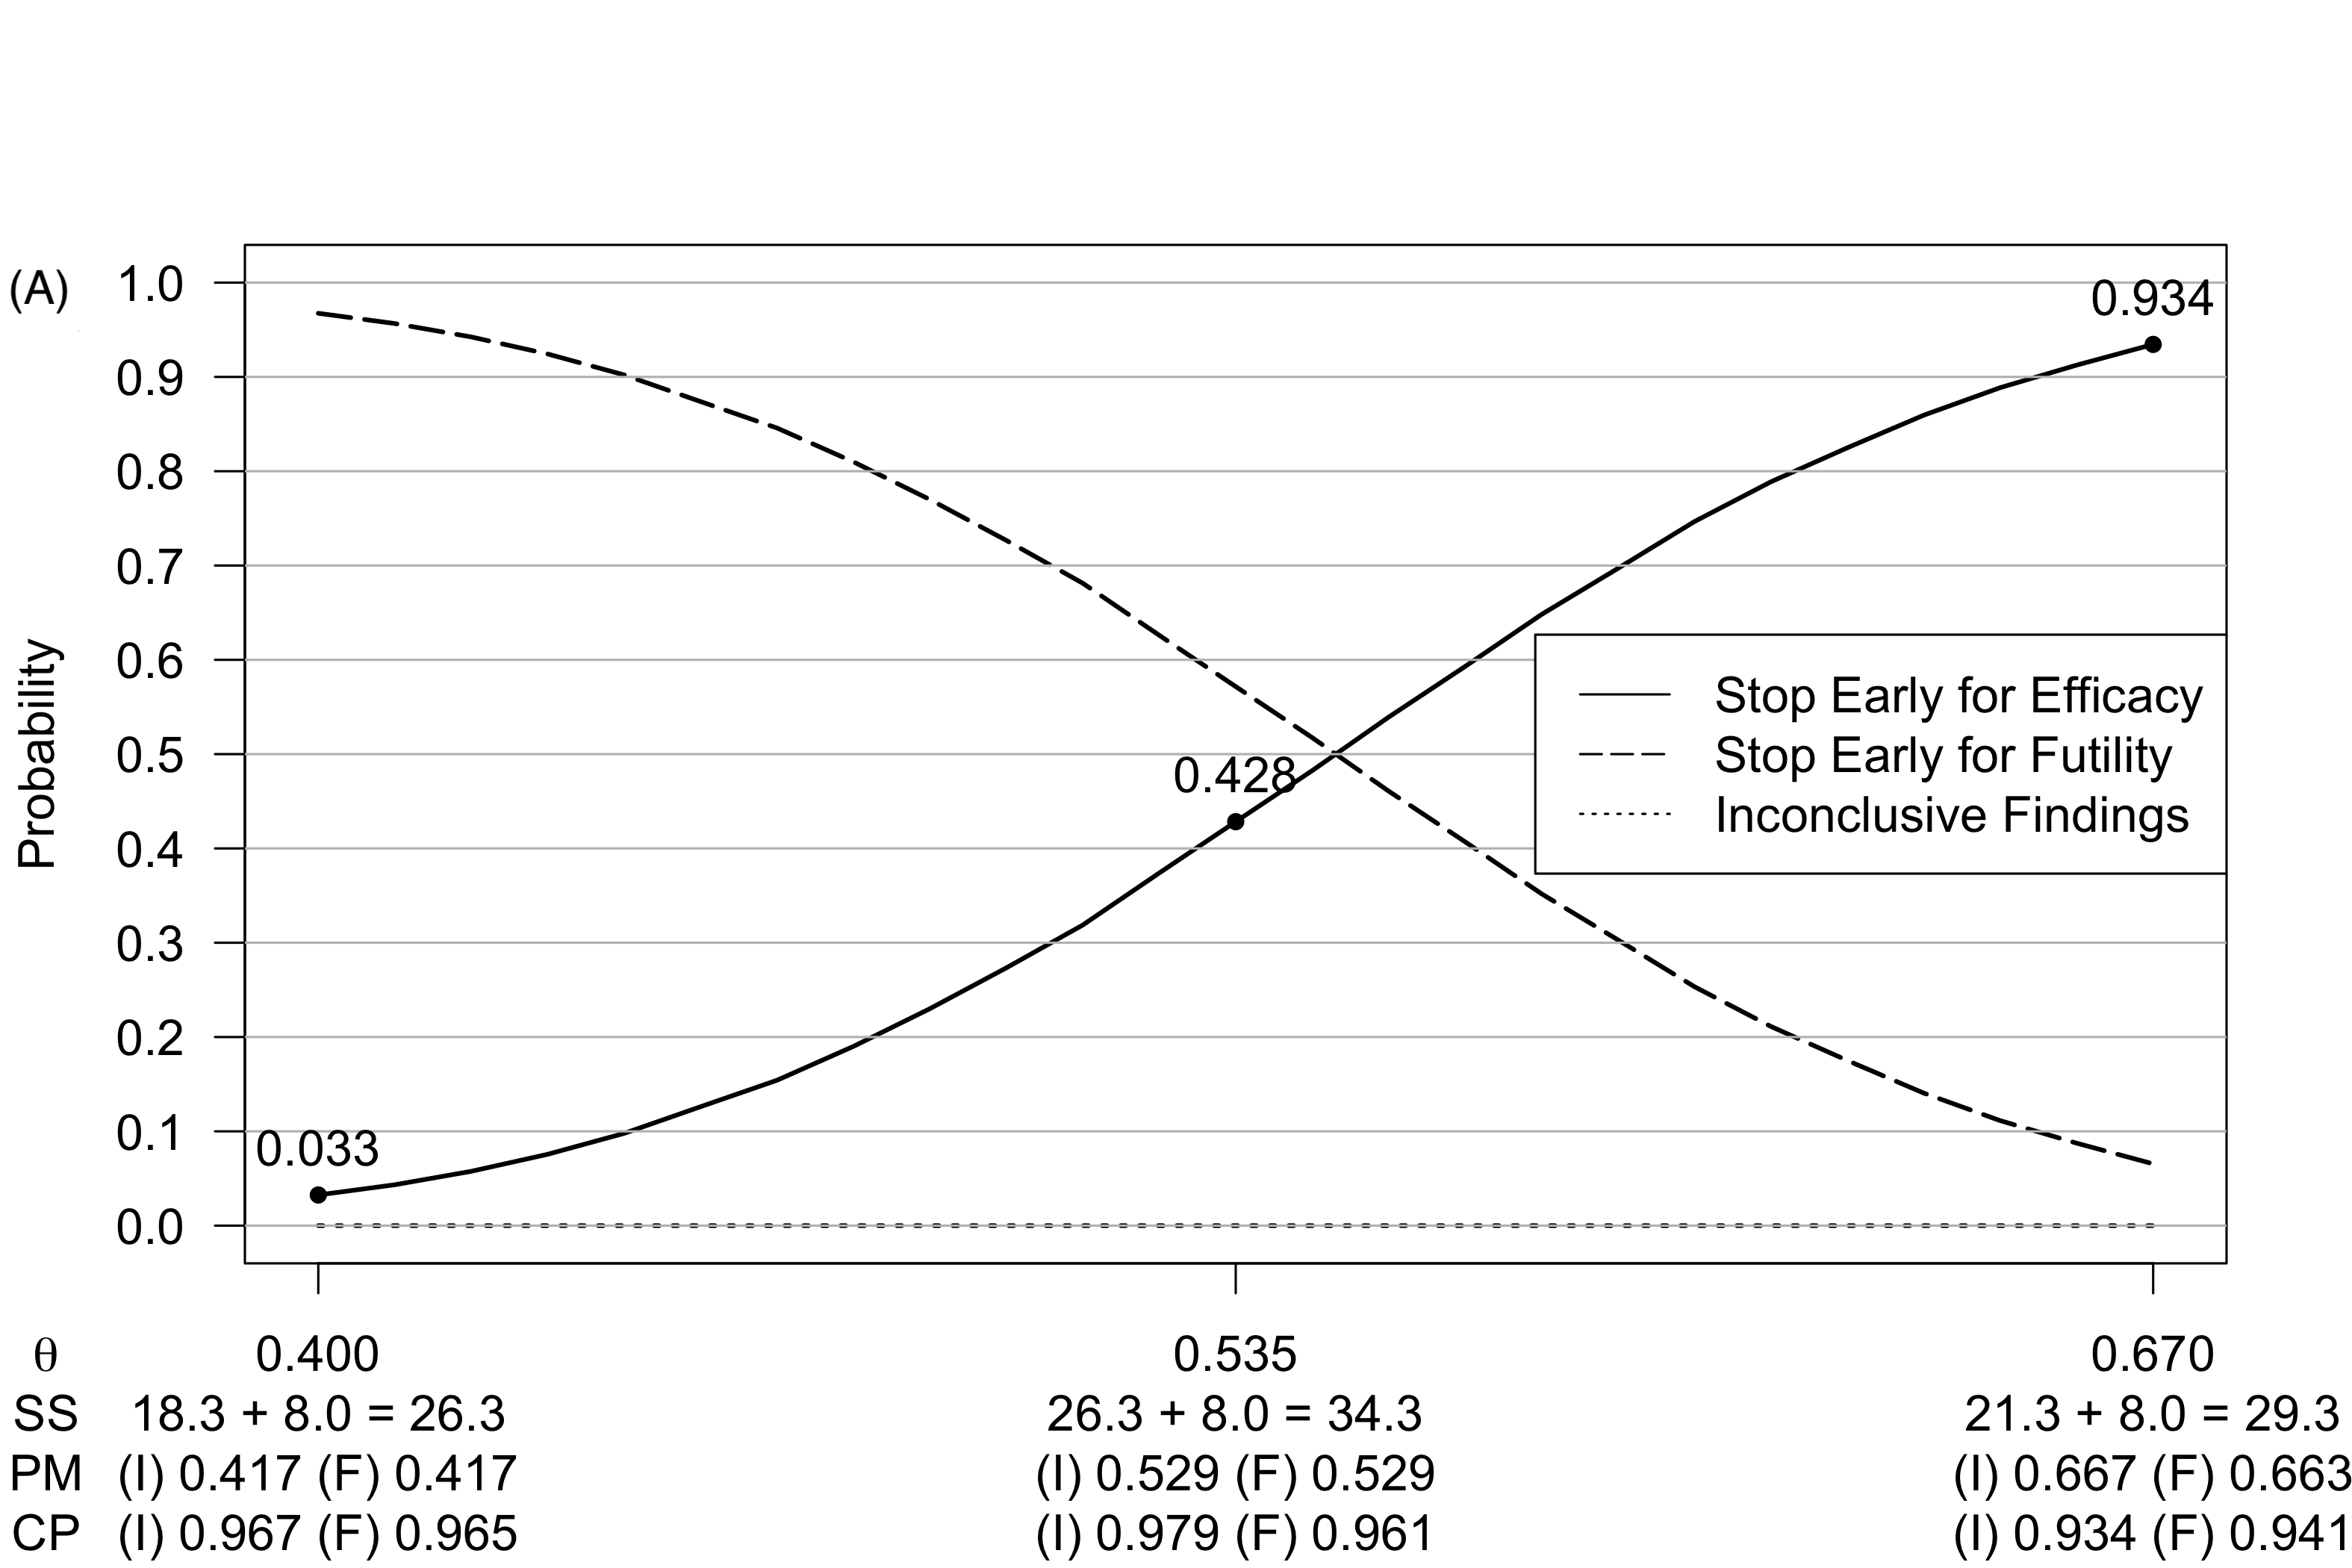
\includegraphics[width=7in]{P:/Bayesian-Sequential-Monitoring/00-paper/FIGURES/figureS2c.png}
 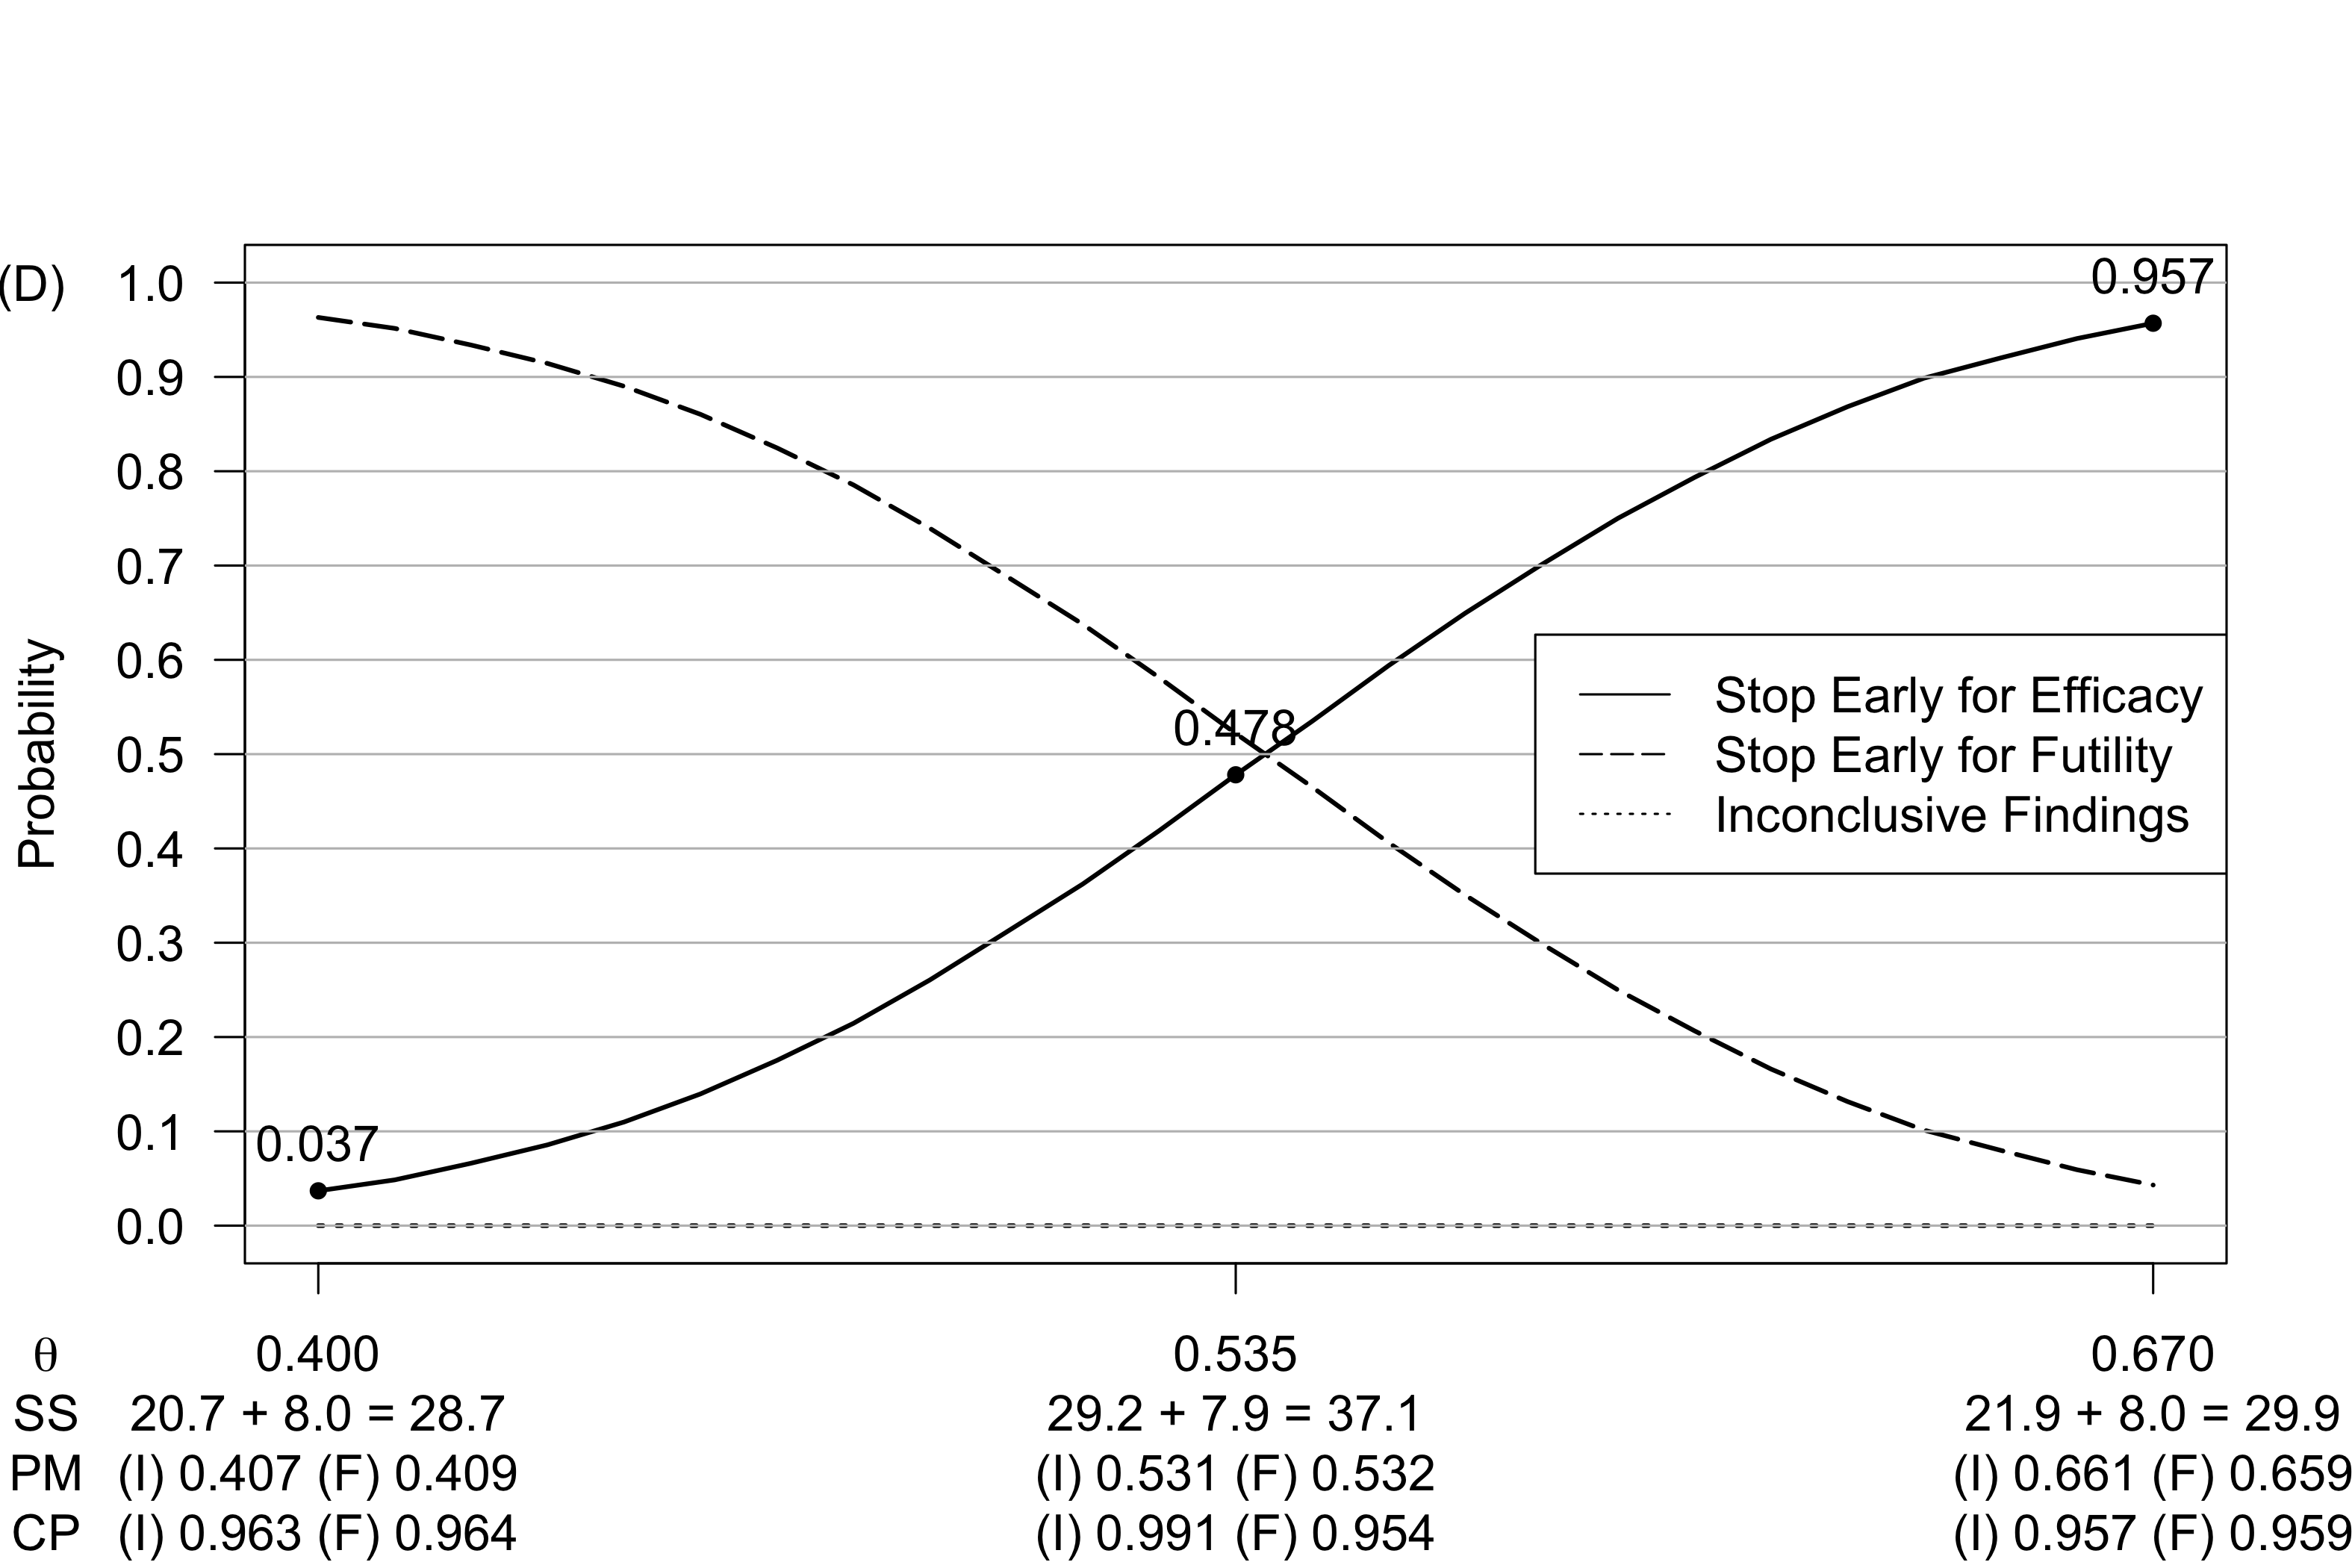
\includegraphics[width=7in]{P:/Bayesian-Sequential-Monitoring/00-paper/FIGURES/figureS2d.png}
 \caption{Modification of enthusiastic prior parameterization in Example \ref{sec:example1}. A, default enthusiastic prior (Figure \ref{fig:figure1}(c)). B, flattened enthusiastic prior (Figure \ref{fig:figure1}(d)). Both designs use default skeptical prior (Figure \ref{fig:figure1}(a)).}
\label{fig:robustness2}
\end{center}\end{figure}

%\section{BibTeX}
\newpage
\newpage
 \bibliographystyle{agsm}
 \bibliography{./References}	

\end{document}
